% $Id$
% Copyright 2005-2010 Lee Gent (lee@leegent.net)

\documentclass[a5paper,titlepage,11pt]{book}
%\documentclass[a5paper,titlepage,11pt,draft]{book}
\usepackage[british]{babel}
\usepackage{microtype}
\usepackage{charter}
\usepackage{graphicx}
\usepackage[tc]{titlepic}
\usepackage[a5paper,inner=3cm,outer=2cm,bottom=25mm]{geometry}

\newcommand{\svn}[1]{\svnsub#1}
\def\svnsub$#1${#1}

\titlepic{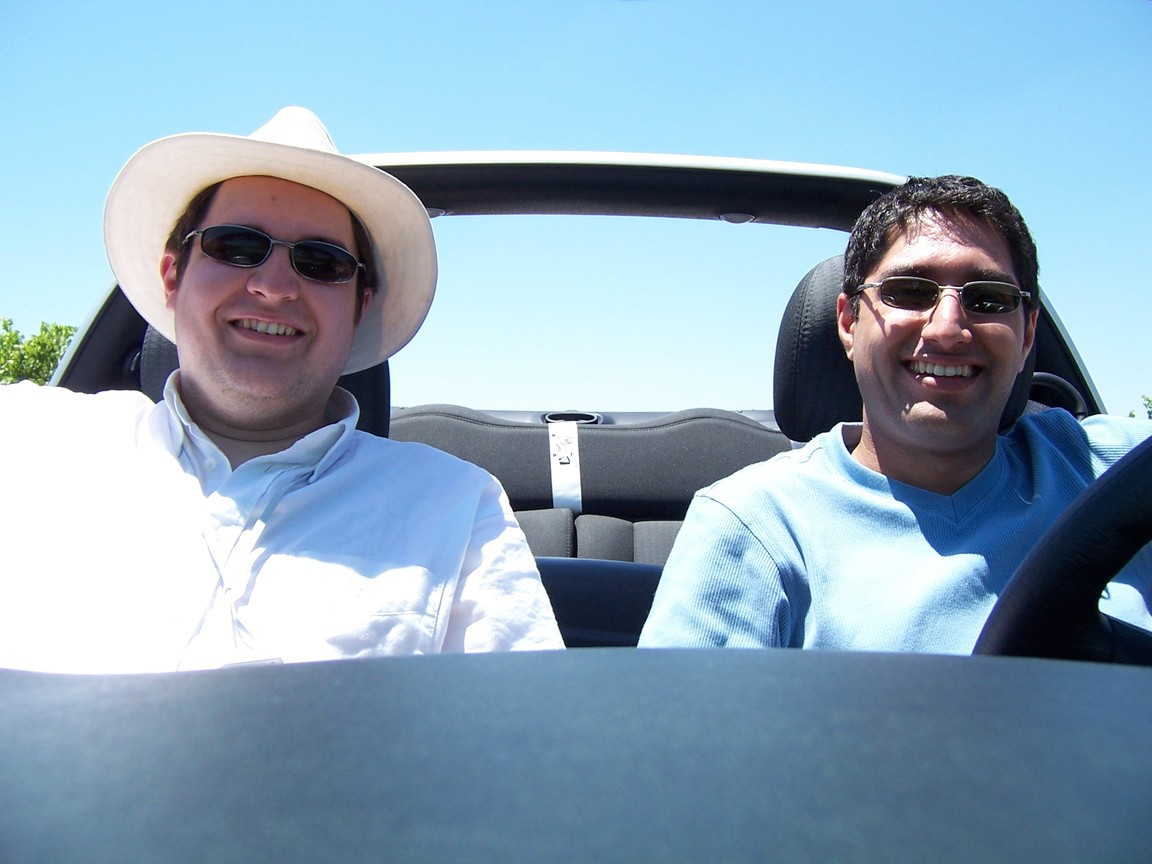
\includegraphics[width=\textwidth]{gfx/title}}
\title{Nevarizonia: An American Road Trip}
\author{Lee Gent}
\date{May -- June, 2005}

\begin{document}
\frontmatter
\maketitle
%\tableofcontents

\section*{A quick note on context}
This was recorded and partially-written in Summer 2005 by an angry, single, 24-year old male.

Some of the thoughts, actions and opinions cause me some embarrassment now, five years later, but I retain them in the name of \emph{science} - this is a close, uncensored examination into the mind of a (and, no doubt, almost \emph{every}) single, angry 24-year-old male.

Gary Glitter had just been sent to jail for being a massive paedophile and Michael Jackson was on trial in California for the same thing.  The most popular thing on television is \emph{The O.C.}  We would see our travels through the lens of these events in the coming weeks.

\vfill
\hrule
\begin{center} {\scriptsize Copyright \textcopyright 2005 -- 2010 Lee Gent \\ \svn{$Revision$} \\ lee@leegent.net }  \end{center}

\mainmatter
\chapter[London -- San Francisco]{Thursday, May 26: London -- San Francisco}
\section*{London}
Day one starts early - 3am for me.  I'd spent the night playing World of Warcraft and so hadn't actually slept much at all - something I thought I could rectify on the long coach and aeroplane journeys ahead of me.

I won't make the same mistake again.

As I wait for my coach I watch the sun rise over the Chippenham countryside and reflect that I made the right decision - the 5.30am National Express is the \emph{only} bus that is \emph{ever} on-time.  It's as though National Express have discovered some kind of wormhole in Space-Time but are too incompetent to use it for good - instead, they use it to slow time down.  The theory goes that, if you slow time down long enough, they can delay the coaches so much that they end up cancelling a service - hence saving money on fuel, drivers, wear-and-tear, that sort of thing.  Clearly, the technicians in charge of the wormhole only start work at 8am - so I get to Heathrow on time - early, in fact.

After a short wait in the brightening sunshine, I'm joined by my hetero life partner, Imran.

We had a brief moment of worry a few days ago when we thought we had to check in at a ridiculously early 8am (for an 11.30am flight), a worry we quickly dispensed with by using that most nonsensical of devices, the Online Check-In.

I'd always thought that the point of checking in was to let the airline know that you were at the airport and ready to rock and roll - not so!  Now you can check in using the Internets - from \emph{miles} away, surely opening hilarious new opportunities for crazy capers like checking in to a flight when you're on the wrong continent.  Ha!  That'll screw them up at the departure gate.

Now, I love Heathrow.  I've only been there twice - last year's trip to Amsterdam and now - and it comes second in my List of All-Time Favourite Places I Like To Pretend Are Some Kind Of Starport, ceding first place to Newcastle's Central Station.

The thing about Heathrow is that it's \emph{bloody} big - even taxiing to the runway takes about half an hour, so long that I thought we were just going to drive the 'plane to San Francisco.  Naturally this is all time you have to spend strapped in, roasting 'cause the air conditioning only works while the engines are ramped up.  Thankfully, Virgin Atlantic's `Attractive Stewardess' policy was in full effect and I am distracted from my discomfort.

There are plenty of good things about the flight, most of which were unfortunately tainted by the single bad thing.  Since I had checked in a little too late to nab the exit-row seats (with the infinite legroom), I foolishly chose the seats behind them, thinking them to be the next-best thing.   The painful reality is that those are probably the worst seats to grab because, presented with all that legroom, the bastards in front of you think it's their right to slam their seat-back down all the way for that As Close To A Bed As You Can Get experience.  You'd think not having to sit in the same place with your knees bent for nine or ten hours would be enough for them, \emph{hell no} - the gits want more.

%If you think I'm being unfairly harsh - after all, the seat backs tilt all that way for me, too, so it's all fair - I say try this:  make fists with your hands.  Press them together and bring them into your chest, so your elbows stick out like wings, or some sort of mutant chicken.  Now imagine you're holding a knife and fork, and you're trying to eat your dinner, but you can't move your hands more than five centimetres from your chest, and \emph{then} you'll see my point.

So, the few good things:  First, the enormous amount of food you're given.  Someone at Virgin had the genius idea of keeping everyone eating, all the time, to stifle boredom.  You are constantly bombarded with pretzels, ice cream, tea, coffee, soft drinks, sandwiches and hot food...  All sorts.  It boggles the mind to think that they store so much food on a 'plane, but it was certainly appreciated.  My eating experience was somewhat stunted, though, since my seat-back tray jabs into my flabby extremities because I'd absorbed all my allotted space like some sort of amorphous jelly-human hybrid.

\begin{center}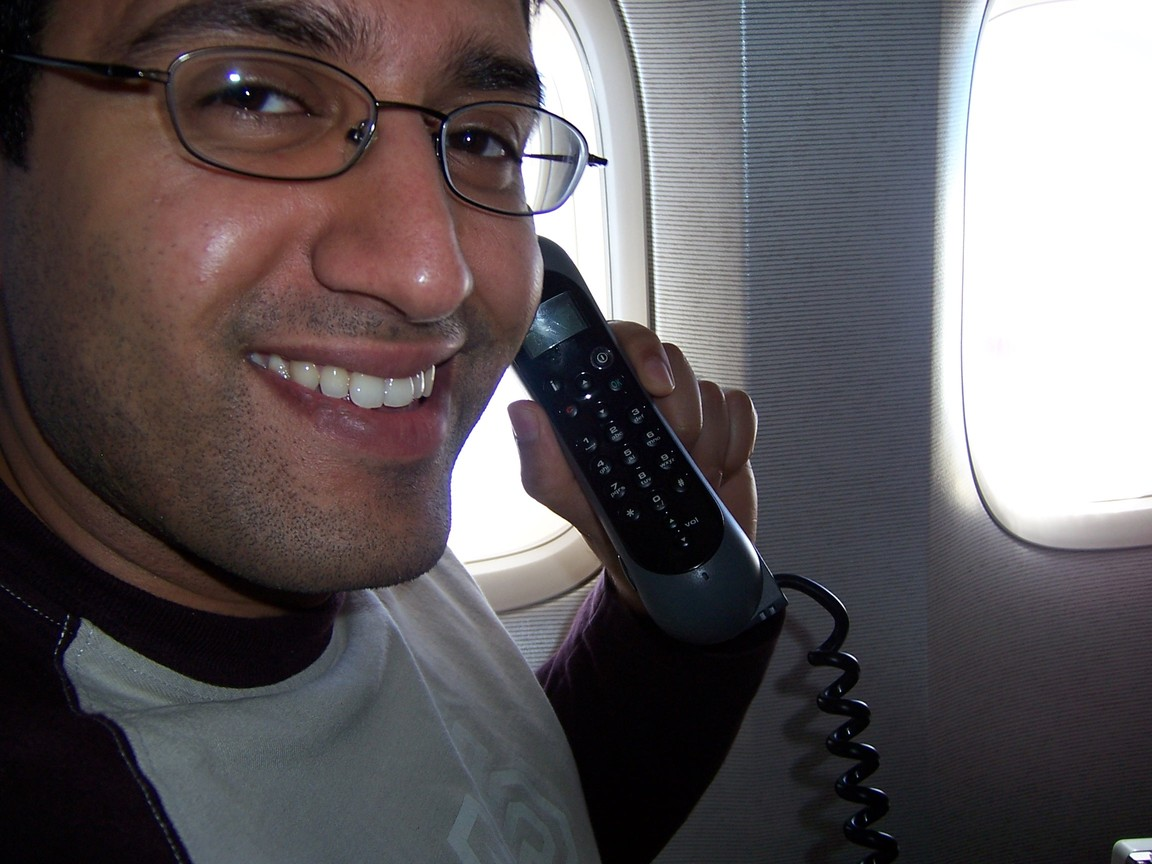
\includegraphics[width=\textwidth]{gfx/100_0991}\end{center}

The \emph{second} and best thing is the in-flight entertainment - a small LCD monitor in front of your face and a pleasingly geeky remote control deck that pops out of your armrest.  Alas, it doesn't come with Mario 3 - first-class only I think, disappointing since I'd planned on playing that for eight hours or so - but it \emph{did} come with a vast selection of films and music, on-demand.  I watch \emph{Team America: World Police} and have to really bite my tongue to keep from laughing during the incredibly puerile (and therefore hilarious to me) bits because I don't want the severe-looking woman sitting next to me to know I am wetting my pants at something so childish.


I follow it up with Michael Mann's \emph{Collateral} and, when that's over, I stick the Linguaphone `Learn Spanish' course on, don the thoughtfully-provided Virgin Atlantic standard-issue eyepatch things and try to grab some shut-eye.

I fail.

\section*{San Francisco}
We touch down around 2pm Pacific Time and soon after we're introduced to the Department of Homeland Security, my disdain for which I'm sure needs no discussion.  At the Customs \& Immigration bit we try to choose the immigration official who we think has had sex most recently, since they're probably the most likely to not hassle us with stupid and pointless questions like `are you planning on conducting terrorist activities' - the answer to which was already marked on my visa waiver card.  On advice of friends and big-ass signs I'd decided against the comedy course of action and ticked the `no, you fucking idiots' box.

Once past America's first line of defense [sic] - ironically a migrant Mexican - we collect our bags and, starry-eyed and in full-on Tourist Mode, I decide to grab my first picture on American soil - the sign saying `Welcome to San Francisco'.  Attracted by the flash, I am \emph{immediately} descended upon by a jobsworth second-line-of-defence, a woman with a serious haircut screaming ``\emph{no pictuuurrres!}''.  She practically manhandles my camera off me and demands that I delete whatever picture I just took. Soiling my pants, I immediately comply - only to find later that my battery had failed a half-second before I hit `confirm' and the picture lived on.  It's published with the rest of my pictures online and I'd like to take the opportunity to say `screw you' to that woman (and that I'm blatantly a raging terrorist).

\begin{center}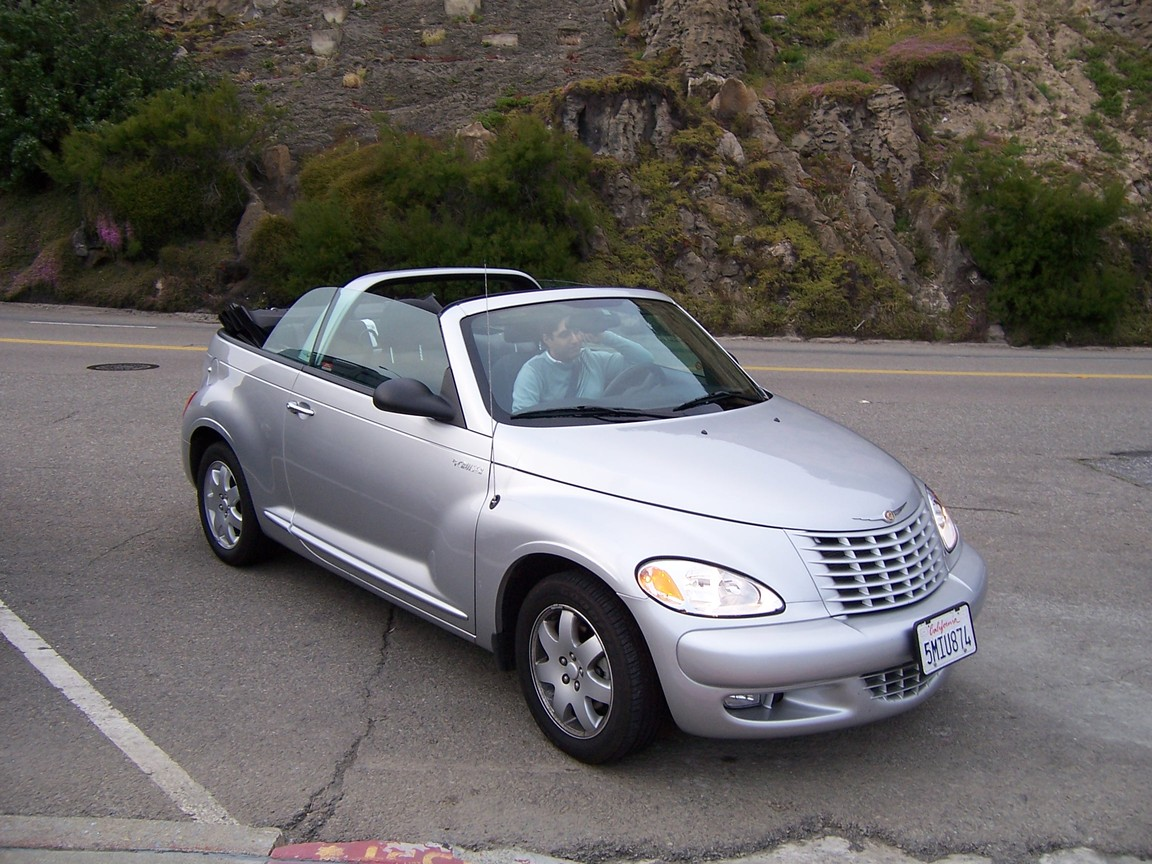
\includegraphics[width=\textwidth]{gfx/100_1064}\end{center}

Onwards we go, then, to Dollar Rent-A-Car.  Now, we've been promised (and paid for) a Chrysler Sebring, a svelte and sexy specimen of a convertible - what we got, after arguing that \emph{no we don't want a sodding upgrade I don't care how much commission you get}, was Herman Munster's hand-me-down - a PT Cruiser.

I'm a guy who appreciates \emph{modern} things, as you may know, so being asked to hang out in this retro beast was anathema to me, and I shed tears.

Thankfully, when you're inside it, you almost forget how monstrously ugly the thing is and easily lose yourself in a world of automatic transmission, cruise control and air conditioning.  Imran drives it out of the underground parking lot and onto the freeway.

The city looms up on the horizon, larger than life, and I whoop and cheer in excitement.

For some reason, I've become my peers' de-facto navigator, probably because I can read a map pretty well (and I rather enjoy that role) - despite the fact I'm usually crap at it.  Thankfully, whenever we get lost, it's always because my map was (a) rubbish, (b) incomplete, (c) not small-scale enough or (d) all of the above.  Naturally, it's never my fault.

The point is, whoever drew my map of the day had decided that I didn't need to know which streets were one-way - as it happens, that's \emph{most} of them - so my carefully-plotted route to the hotel turns into a `fun' cruise around downtown San Francisco.  In rush hour.  Which eventually terminates in what would later turn out to be the \emph{wrong} hotel.  We find out later that there are two `wings' to the Holiday Inn and the one we were booked into (and, incidentally, the one which offers guests free parking) is across the road and facing the other direction.  This explains why the \emph{utter idiot} attending to us has absolutely \emph{no} idea who we are, who Virgin Holidays are or where we could park.  Eventually he checks us in and charges us seventy dollars for parking.  

We spend the remainder of the evening exploring.  Naturally, we cross the Golden Gate Bridge and stop on the other side to look back and take in the cityscape before we realise that we'd both forgotten our cameras.  Loath to pay the five buck toll to cross it southbound into the city and, in the first of many instances of what we'd dub the `Scale-Spaz' - the failure to correctly translate distances on a map with \emph{actual} Space - we decide to just carry on exploring, with me foolishly assuring Imran that I can plot a long, exciting route back along the shore of the Bay and home across the Bay Bridge, many miles away.

I probably could have done it given six more hours but all too soon it began to get dark, our stomachs start to rumble and sleep seems to be dangerously close.  In the end, we end up having a lovely tour around Sausalito and the southern marches of Marin County until we are forced to turn back.  As penance, I pay the toll to cross the Golden Gate Bridge again and we return to the city.

We park up somewhere around City Hall on the way back and eat our first real meal Stateside - pizza in a nice posh restaurant.  Six months later Imran would receive a parking ticket for this.

We are beginning to get the hang of the streets here and handily navigate our way back to the hotel for some real sleep, and not a moment too soon - we're so exhausted we've started to have microsleeps at the wheel.

\chapter[San Francisco]{Friday, May 27: San Francisco}
An early start thanks to jet lag, and out onto Fisherman's Wharf to find breakfast.  Briefly contemplating the strange hollowed-out bread bowls full of a viscous creamy liquid not too dissimilar to wallpaper paste (turns out it's clam chowder which apparently the region is famous for), we found what we wanted - a retro 50s diner, with free refills on coffee (damn you UK, you need to catch up on THIS one) and that most bizarre of breakfasts: pancakes with massive slabs of lardy butter, syrup and teeny tiny bits of nuked bacon, cheerfully delivered unto me by a friendly Mexican chap.  I didn't want pancakes, but it was the only thing for breakfast that wasn't based on eggs.  Breakfast-sans-eggs clearly isn't a popular choice in the colonies.

Eager to plan ahead, we ask our waiter for advice but, unfortunately, he is too young to helpfully advise us on possible drinking venues for later.

Thankfully, my map de jour is decent and we find our way to San Francisco's famous cable cars - where it dawns on me that these cars were strictly stuck to terra firma and merely propelled by a wire in a city-length underground pulley system.  I stop looking for the kind that hang from wires on ski-slopes.

Easy mistake to make.

After a full twenty-four hours Stateside, we are terribly disappointed with the lack of eligible bachelorettes - we'd both swallowed the Hollywood idea that everyone in the US is beautiful - although it's true that their teeth \emph{are} better than ours.  Anyway, we finally meet our first attractive female - she tries to get us to subscribe to her charity of choice in the Market district.  I lie and say I already send money to Greenpeace, then take her picture.

\begin{center}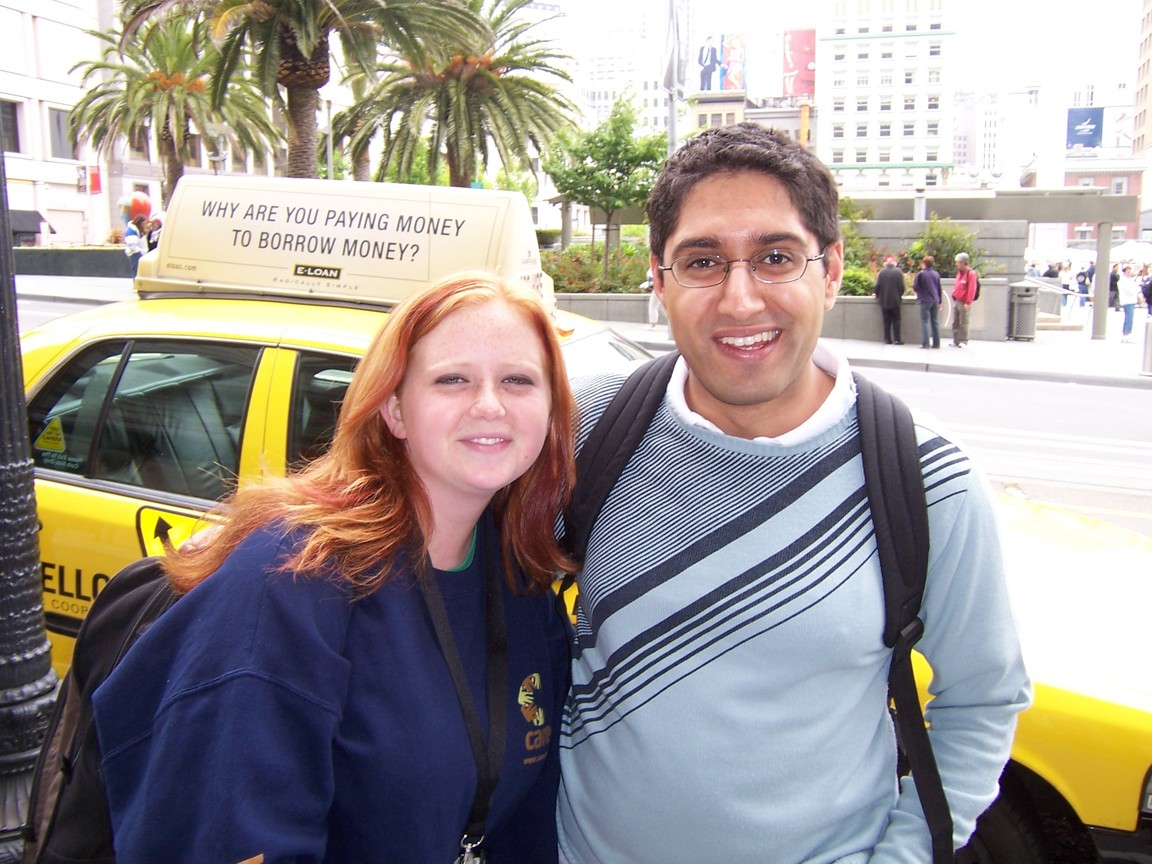
\includegraphics[width=\textwidth]{gfx/100_1016}\end{center}

All in all, we visit:
\begin{enumerate}
\item A shop full of beauty products - Imran likes to look beautiful; I like to look insecure and uncomfortable, so it's win-win.

\item The Apple Store, which is a let-down because it is small (we really expected a larger store this close to Cupertino), dull and, damningly, not actually all that cheaper than the UK thanks to sales tax. No merchant in America ever adds sales tax onto their ticket prices, clearly just to screw over unwary tourists used to bizarre, socialist concepts like putting the \emph{actual} monetary cost of a product on the price tag.  It was also staffed by an army of so-trendy-it-hurts fashion victims who I immediately wanted to punch in the face - much like Gap, only with less useful products.

Now, my trusty iPod had \emph{totally} died the night before I left, which in a way was handy because I feel less guilty about buying a replacement.  With 20Gb not being big enough for my current library plus future expansion, the iPod Photo being overkill (why on Earth would anyone want to look at Photos on an iPod?) and the Shuffle being waaaaaaaaaaaaaay too small, I decide that maybe I \emph{can} live without having my entire collection attached to me all the time and finally spent my hard-earned Benjamins on a 6Gb Mini.  I briefly consider not bothering with the iPod and getting a competing brand before remembering that I'm hopelessly addicted to the iTunes Music Store.

I fondle the Mac Mini for a minute before I suddenly realised that it is, in fact, rubbish and hugely overpriced - a realisation swiftly followed by the ``actually, this is ALL rubbish!'' thought, which rather neatly quantised the let-down feeling I had - the Apple Store was rubbish because \emph{Apple only make four or five products}.

Despite this, I still buy a lanyard for my new iPod, but only because I have a thing for lanyards akin to my love of Panama hats.

\item Old Navy.  I've no idea where on a scale of 0 to Trendy this store lies, but I spend forty pounds on clothes anyway - including a fetching pair of Stars and Stripes boxers which I duly appoint to the office of Lucky Underwear, the incumbent pair retiring citing stress and a desire to spend more time with his family.

\item A pharmacy, where a pleasant Mexican man sells me throat soothing sweets to combat the cold that has been growing since sharing a cramped aeroplane with (and breathing the recycled air of) four hundred people for eleven hours.

Later it would dawn on me that the number of pharmacies in the US easily dwarfs the number of schools and libraries - they \emph{do} love their drugs.  There were even \emph{drive-thru} pharmacies.  I struggle to conceive of any scenario where the need for drugs is so great that patrons don't even have the time to get out of their \emph{car}.

\item Skechers.  I had bought a pair last year in Amsterdam and they were easily the best pair of trainers I've ever had.  After that experience, Skechers ousted Nike - who are too busy making luminous green foot-turds these days - as my trainer of choice.

Since the closest stores in the UK are London and Birmingham, I'd been itching to grab a new pair for a while and now I had the perfect opportunity to replace the flimsy pair I'd brought with me.  They were \textsterling4 from Asda and had looked the part but they contain exactly zero cushioning and were therefore nothing but slightly less-fluffy slippers - not terribly ideal for walking on pavement with.

Again, the serving monkeys are of the too-trendy variety and seem to find something about me or my accent enormously amusing. From time-to-time they go behind the counter to huddle and whisper to one another, occasionally looking back at me and giggling instead of getting my goddamn trainers from their goddamn stock room.

I pay them back by liberally wafting my foot-scent around their pokey store.

\item Macys, where we spend a good deal of time at the sunglasses and toiletries bits at Imran's behest.  Or, rather, Imran spends a good deal of time talking to the serving ladies in a language I don't understand, Trendy, while I look at absurdly expensive smelly water and try to avoid the aged, heavily made-up ladies trying to douse me in the stuff. I show my ignorance by proclaiming loudly `no thanks, I don't wear aftershave' (it's eau du toilette, dahling).

\item Virgin Megastore where, buried at the back, they have a `British' section which sells Heinz Baked Beans.  We are most confused; surely they have beans in the US?
\end{enumerate}

\begin{center}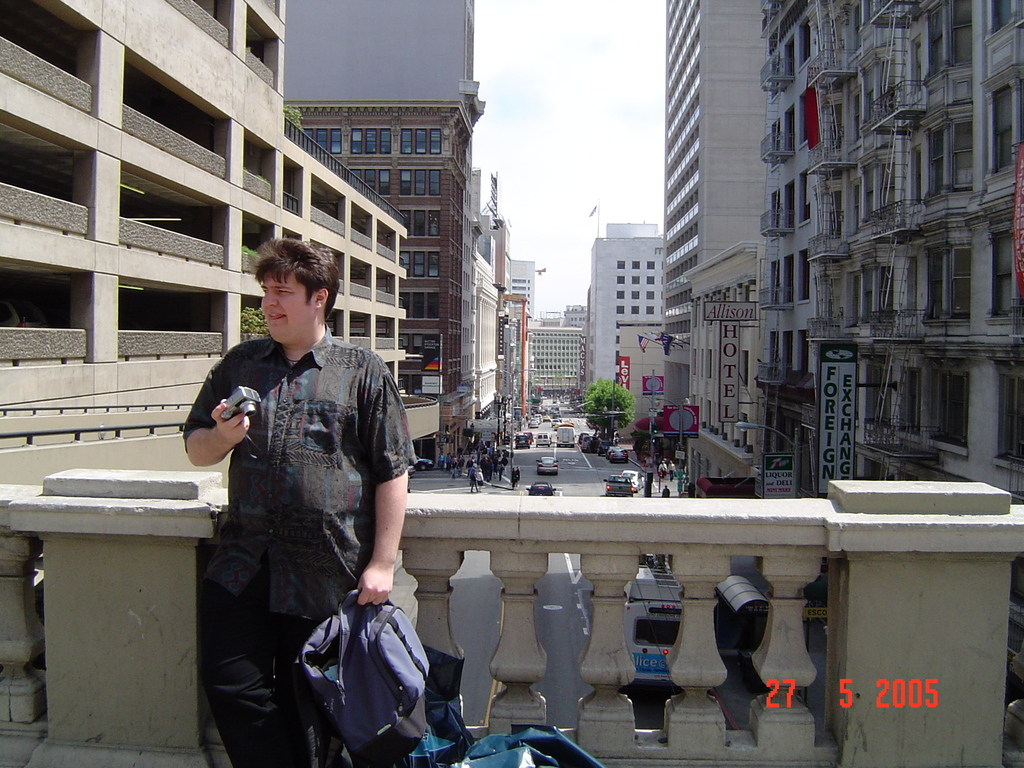
\includegraphics[width=\textwidth]{gfx/DSC00625}\end{center}

We enjoy a tasty lunch somewhere in Chinatown and begin to walk back to the hotel, spamming up and down those famous, big-ass hills - they're not quite as cinematic when you've got to trudge up and down them repeatedly.  Both Imran and I are fascinated by the frequent juxtaposition of wealth and beauty against down-and-outs, and occasionally stop to take pictures of hobos.

As we ascend the last hill, the noise of rock music drifts down the street towards us.  At first we think it is some inconsiderate moron with his window wide open but, as we near its source, its true nature became apparent - it is live music, live \emph{rock} music, and it is coming from a \emph{car park}.  We eventually realise it's not quite as random as we thought - this is the car park of a large yellow building emblazoned with `Tower Records'.  We watch the remainder of the band's set with the large crowd of people gathered, gyrating to the catchy choons.  The music is very good and, when it is over, we learn that it is none other than Jackie Greene - who we've never heard of.  Enchanted by what we'd just heard, we both enter the building, bought his CD and had it signed by Jackie himself.  For shits and giggles, we promise we'd try to make him famous in the UK before realising that he is, in fact, a massive primadonna douche-bag who wears sunglasses indoors, soaking up praise and adoration while his poor bandmates, skilled musicians down to a man, pack up the gear outside.  To make their day, I stop them and thank them.

I'm like that, you see - always rooting for the underdogs.

We wrap up the afternoon by taking a drive around the city again, this time heading west to check the Pacific out (the Pacific! I've waited years to see it).  We drive past Eastern Orthodox churches and buildings with enormous rainbow flags hanging off them, eventually deciding to whack one of our new Jackie Greene CDs on the car stereo.  Unfortunately, rather than the rockin' stuff we'd heard earlier, the CD was entirely whiny, soft-ass guitar noodling and substandard jazzy blues - not even the kind of whiny soft-ass rubbish that I ordinarily \emph{like}.  That bastard tricked us!  Boycott Jackie Greene!

The Pacific coast isn't at all what I was expecting - at the western edge of San Francisco it is kind of dull, rugged and cold.  I console myself with the thought that San Francisco has it's own microcosmic weather system and that the rest of the coast is probably all shimmering sand and palm trees - just like I've been led to believe it is.

At the coast we head south and entertain vague notions of going all the way to Silicon Valley but realise that, once there, we'd have literally nothing to do but get out of the car and go `yep... Silicon Valley...'.  Instead, we get a little lost and, with time running out as usual, turn north and try to head back to base camp via the absolutely wonderful Embarcadero.

\begin{center}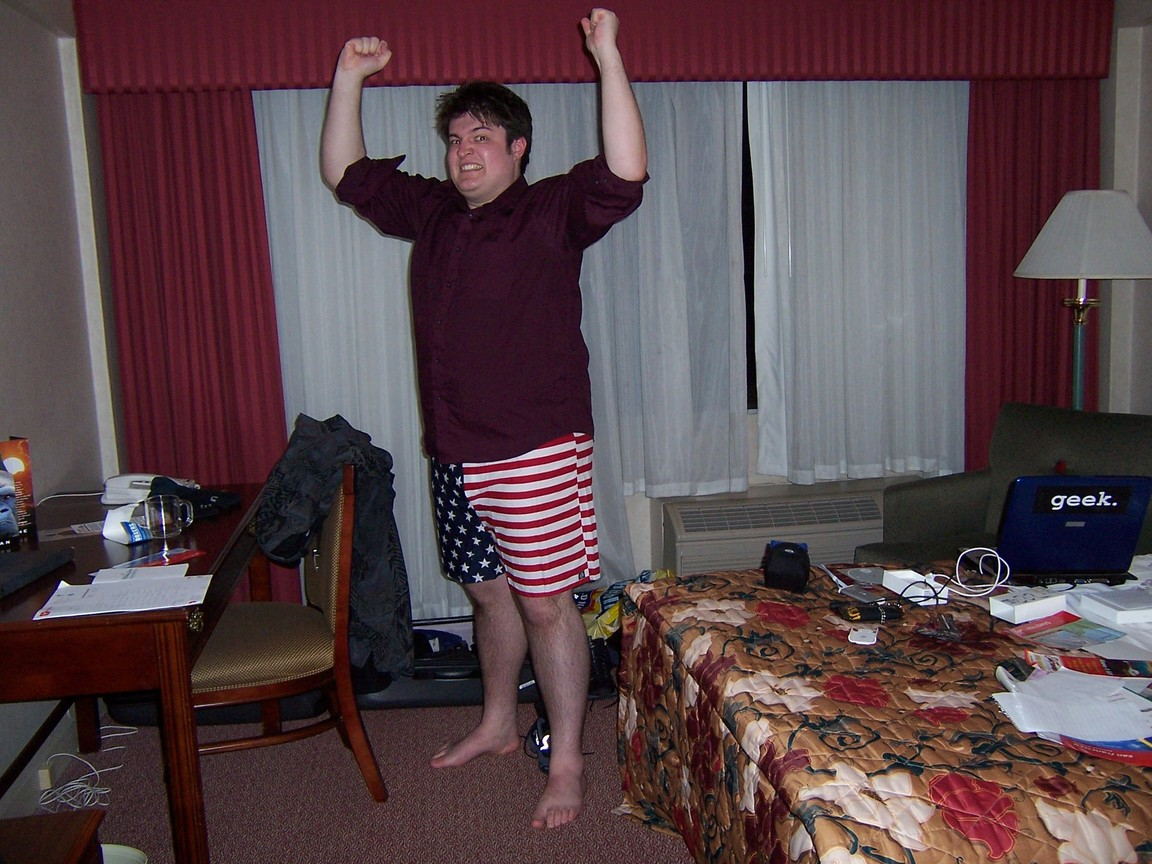
\includegraphics[width=\textwidth]{gfx/100_1097}\end{center}

On the way back to our hotel we pass a \emph{Hooters} and decide it would be a great yarn to grab some dinner there - to do something \emph{really} `American'.  We head there after showering and breaking out the party clothes - including, of course, my latest pair of lucky boxer shorts fashioned out of a Star-Spangled Banner.  I stop short of pasting George Bush's stupid face on my arse, though.

Hooters isn't at all what we were expecting.  Sure, there are beautiful, scantily-clad, lithe and full-bosomed serving wenches - but are were also a large number of \emph{families}.  People take their \emph{kids} to Hooters, which totally ruins it for us - no \emph{way} is it possible to enjoy such sights properly when two tables down is some kid's birthday party.  There are even sad old men watching \emph{sports} on the TV in there, for goodness sake - don't they have a TV at home?

You see, for me personally, the appeal of Hooters' principal selling point is somewhat lesser than it is to your average male, simply because I'm usually indifferent to any woman I know I have no chance of ever being with or, more relevantly, I'm immune to women who are \emph{paid} to be friendly with me.  I am, therefore, fully able to resist the busty maidens' blatant and incessant fishing for tips; right now, I'm here for the food.

Perhaps it is wrong of us to expect good food at Hooters, and even wronger of us to base our opinions of the place on the food rather than the... well, hooters, but it's hard to like a place that serves chicken wings which are 95\% gristle.  The menu does not list Cod but `Cousin of Cod' - I ask our waitress but the best she can offer is ``well, it's not actually cod - it's just \emph{like} cod''.  They have switched it for a similar, cheaper fish and - guess what?  You can tell.

We eat our side-salads instead and prepare to leave.

We've been in town for forty-eight hours and have already learned a valuable lesson - \emph{all} the food seems like it is crafted from blocks of lard.  Even the \emph{vegetables} have been loving painted with butter.  That stereotype about `meals are bigger in the US' isn't true - it just feels that way because you're eating raw fat.

It is our intention to go clubbing and meet people of the opposite sex and so, before we leave, we ask our reasonably attractive (but obviously angry at the tiny, contemptuous tip we'd left her) waitress where to go out in the city - she offers one possibility but confesses that she does not know of anywhere that might suit us.  After a hasty retreat, we walk aimlessly for a little way before we're able to grab a cab and order the cabbie to take us to \emph{women}.

What we didn't expect was to pick the cab of the most useless taxi driver in all of San Francisco - I didn't believe it was possible to meet a cab driver who didn't know where young, cool people like ourselves hung out (``what do you mean you don't know where hot women hang out?  Don't you spend all damn night picking them up from places?'').  Thankfully, after collating our intelligence we pick our way to where the nightlife seems to be centred (somewhere just north of Market Street) and attempt entry into the club our Hooters girl had recommended.

We don't actually get very far because the bouncers turn us away, curtly informing us that we'd have to wait - goodness knows what for, because the place is painfully obviously \emph{dead}.  We shoot them a `well-I-shan't-ever-come-back-here-I'm-British-you-know' glance we instead decide to waste our time in the pub next door.

Big mistake.

Picture a small, seedy sports bar.  Turn all the lights down reeeeeeally low.  Place six or seven one-armed bandit things and assorted football arcade machines down one wall.  Add two filthy pool tables, and a few ancient CRT televisions spewing out baseball with a hint of purple 'cause the tubes are shot, some more dirt, some nice `generic rock music' - the kind that makes backing tracks on, well, sports videos or Monster Truck shows or something - and \emph{biker dudes}.

I had my doubts; Imran kinda liked it.

After getting some `drinks' and peeling my hands from the sticky bar, we found a table to chill at, recently vacated by some smelly biker rock sports-fan dudes.  I instantly realise that I physically cannot not fit in the gap between the nailed-down table and fixed seat.  By now, though, it is too late to turn back and people are starting to peer at us strangely.  Out of options, I suck in my swollen gut and just \emph{go for it}, managing eventually to wedge myself in but not before noisily and embarrassingly knocking a drink over, and not with the room required to actually \emph{breathe}.

We drink our piss-like beer in silence while I slowly turn blue and keep an eye out for some redneck biker to stab us for being in his regular seat, but it makes us ill (probably because it was piss, \emph{actual} piss - it was that kind of place) and we take our leave.

Just to spite the dumbass doormen who denied us entry to our first intended destination, we cheerily stroll right past them and onwards towards a club that had actual \emph{people} outside.  But what's this?!  Guest list only?  Not to worry, our man Imran (as ever) has some tricks up his sleeve.  Addressing the guestlist-gorilla in a perfect smarmy minted City-worker accent, he proclaims that he'd heard of this establishment even as far as England, and that it came very highly recommended, and we'd travelled \emph{so} far to check it out.

Quickly elevated to Guest List status, we enter in, do a quick reconnaissance sweep and settled down to get blotto and try to chat up girls.

It wasn't long before we are approached by an attractive, pleasant girl who takes a seat beside us, introduces herself and makes smalltalk - whereupon I instantly tune out as I hadn't yet reached my witty and entertaining state of mind.  A fine start to the evening, we thought, until it started to become clear exactly what Jamie-Lynn was - a \emph{vulture}.  A saleswoman working for the bar whose job it was to entertain and manipulate people to get them to buy inordinately overpriced drinks before schmoozing off to ply her wares on other groups of unwary y-chromosomes.

We fall for it the first time, eventually giving in to her regular `can I get you boys something to drink?' promptings, and she took off to get us a couple of Budweisers which, bizarrely enough, don't as much like urine as they do in the UK.  Well, \emph{usually} - because once again we'd been bestowed with disgusting swill.

It takes us nine tenths of the bottle and great deal of protesting from both our stomach linings before we realise that we'd been given \emph{alcohol-free} beer.  Great!  Now you too can drink excrement and not even get drunk!  What a wholly pointless exercise!  Eventually she comes back (although I suspect only because our bottles were on the wrong side of full and she can smell a sales opportunity - mistake!) and we make our disgust very clear.

After much haggling, wailing and gnashing of teeth, she get us some full-fat beer (well, Bud again - sigh) - and never speaks to us for the rest of the night.  Later we would realise that maybe we were a little harsh on her and the reason everything we drank that night tasted unpalatable was probably Hooters fault.

By this time, the club has begun to fill up a little - with \emph{frat boys}.  They are real and they're every bit as obnoxious as you'd expect a bunch of lightweight college jocks to be - and we wanted them to explode.  Eventually they didn't, and we turn our attentions to a group of young ladies who'd decided to sit close and make the foolish mistake of making eye-contact - clearly our cue to plot an intercept course which, true to form, we did.

Again, I check out during the initial smalltalk - I'm not in the mood and seriously lacking mojo.  Instead, I have a go at playing the dark, intense, moody guy card (the card I'd played most nights out since 1997) while Imran makes some headway with an easy-on-the eye lassie who, alas, didn't instantly melt at our accents.  Unfortunately, that was the linchpin of our strategy.

While I sip on my Bud and put on face \#51 - `Sly Grin As Though I'm Laughing At Some Private Joke Because I'm So Carefree and Laid Back', I notice that most of the girls have rings on their ringfingers.  Are they married?  I panic a little but realise that they don't really look like wedding or engagement rings and so I ask if they are used to ward off potential suitors - apparently not.  They are simply items of fashionable jewellery.  Imran and I make mental notes to ignore any and all wedding rings.

My partner-in-crime suggests a dance and steers his lady to the dance floor while I hold the fort with the remaining ladies.  Tonight, though, it seems I am powerless and they slowly start to marginalise me.  Eventually, after I simply lurk on their periphery for an uncomfortable and downright embarrassing length of time, they all decide to intervene and move to the dancefloor themselves before marginalising Imran as well.  Time passes and he returns, defeated, while the entire group of ladies move far away from us - to the back of the bar, wherein lies the frat boys.

After a last overpriced beer, a final scout around and finally coming to the conclusion that no new, cool people were entering, I grab Imran and we leave, seeking more fun and frolics on the streets of San Francisco.  There were some strip joints (``no'', I said - ``we won't find any hot single women there, will we''), some slightly trendy places that were empty and a few nomadic groups patrolling up and down.  By this stage I've finally imbued enough to think it's socially acceptable to stop random girls on the streets and scream ``WHERE'S THE FUN AT?  WHERE ARE YOU GOING?  CAN WE COME?'' - a technique which, as you can imagine, fails to have the desired effect (`ooh, what a kooky, confident English guy, that's kinda cute, let's hang out') and instead, well... chases people off (`oh Christ he's talking to me, let's get the fuck outta here').

There was some action though - a fight.  Just your average drunken brawl in the middle of the road - heck, we even had those in Ponteland - except when the bouncers intervened, it became clear that the bouncers were \emph{packing heat}.  This drove home the point that the country was just as strange and unfamiliar as anywhere else beyond our nice, safe borders - and they speak English to \emph{deceive} us into thinking that we could almost be in England.

We took a taxi home and, once home, discuss some observations and opinions we have formed so far - both of us expressing distaste at some elements of the American way-of-life; at the crazy television with adverts every five minutes, Fox News and their campaign to turn everyone into xenophobic automata and just how central to some American's lives pharmaceuticals are.  Every third advert is for some sort of wonder-pill.  Every third strip-mall has a drive-thru pharmacy the size of a stadium.  Every problem can be solved with drugs.

Oh, and US TV adverts are allowed to bad-mouth their competition, by name.  It's almost funny to watch some guy mockingly proclaiming ``Biz Automatic can't get rid of THESE stains, because it's shit - but OUR stuff can!''.  Naturally, said guy has to have dubious academic credentials subtitled on, along with his name - \emph{like anyone cares about his name}. ``Hi! I'm Dr. Doug Arseburger [subtitle: Doug Arseburger Ph.D, Leading Cheese Researcher], and our cheese is far better than that crap Cheese, Inc. make'' and so on.

It's also bizarre to see just how low-tech your average dude-on-the-street is.  Walk around somewhere as backwater as Chippenham and even here there are hundreds of those damn white earbuds that USED to say `I'm a pretentious new-media whore' but now say `I'm the same as everyone else' - what we saw in our travels were hundreds of people still with old-skool cassette Walkmans.  It was like the 80s all over again, only less crap.

We succumb to sleep's blessed embrace.

\chapter[San Francisco -- Yosemite]{Saturday, May 28: San Francisco -- Yosemite}
\section*{San Francisco}
At this point I'm still a hotel noob and genuinely believe that if we fail to hand our cheap plastic keycards back to the reception desk before checkout time, \emph{terrible} things will happen.  Naturally, then, I spend the former half of the day fussing and worrying as we go renegade, Imran assuring me there's no need to return and we should abuse the free parking a little longer.

Immediately north of us is Fisherman's Wharf where we find a caf\'{e} on a pier.  Breakfast is fresh coffee and clam chowder in bowls make of sour-dough; it is \emph{sublime} if not a little cold and windy.

The USS Pampanito is moored close by - she's a World War Two-era submarine that's been converted into a museum. After enjoying the view of the Bay and Alcatraz, we head inside for a bit of history, briefly stopping to shake my head at a comment book entry by `Cindy, Palm Springs, CA'.  Amongst comments like `it's a privilege to be here', her comment reads simply: `this sux'.  Bless.

We stroll around the shops.  Ever the fashion victim, Imran tries on and discusses the relative merits of a succession of obscenely expensive designer sunglasses with a decidedly dodgy Russian dealer.  His Oakleys just aren't trendy enough these days, but a pair of Raybans will fill the void nicely.  I begin to feel a little dirty, wielding my \textsterling9.99 `no protection, guaranteed' pair from Burtons.

The Russian dude knows his onions and prompts Imran to go in bold new fashionable directions (``people think because you have a small face, you have to have small glasses -- try these \emph{large} ones!''), which he does before eventually (and amusingly spontaneously considering how long we looked and deliberated) settling on a pair.

The Russian guy rubs his hands, because it's now time for the \emph{real} selling to start - price negotiation time.  These specs are top of the line and have an accordingly vast price tag, but our man Imran is just as shrewd as our Soviet buddy and eventually a lower price is agreed - but wait!  We have one trick left up our sleeve.

``Aww, I forgot about the sales tax'', fakes Imran.  ``Such a bummer.  I'm not sure I can afford it now.''

With a furtive glance left and right and a faintly discernible screwing up of the face while he eventually decides we're not IRS agents, our comrade lowers his voice and whispers, ``...you pay cash?''

With the faintest of smiles, Imran nods.

``OK.  Pay cash, you pay only ninety dollars...'' There's a pause, and we expect him to finish his sentence with ``tell anyone, and I slit your throat while you sleep''.

It doesn't come to that, thankfully, only I begin to feel some throat-slitting action is imminent as it turns out Imran has forgotten his wallet.  He must now run all the way back to the hotel to fish it out while \emph{I} have to stand around the tiny, empty store looking sheepish.  Russian dude isn't best pleased and briefly considers murdering me and selling my organs on the black market before again convincing himself that this isn't an IRS sting operation and we really ARE hapless limeys.  He promptly tries to sell me some new specs which I wriggle out of buying by convincingly telling him that I don't ever actually go `outside'.

One successful bit of commerce later, we jump into the MunsterMobile and hit the road - it's time to do some `\emph{Bullit} shit', by which we mean zoom around the famous streets and hills of 'Frisco.  First stop is one of the highest points in the city, the Coit Tower on Telegraph Hill, but there's a mammoth queue.  We give up and decide to snake our way down Lombard Street - apparently the most crooked street in the World - much to the disdain of a traffic cop at the bottom.  As we crawl down taking pictures, she commands us to go faster and get on our way with a look that could easily, even seen from a moving vehicle coming down a bendy hill, have said `f'ckin' tourists'.

\begin{center}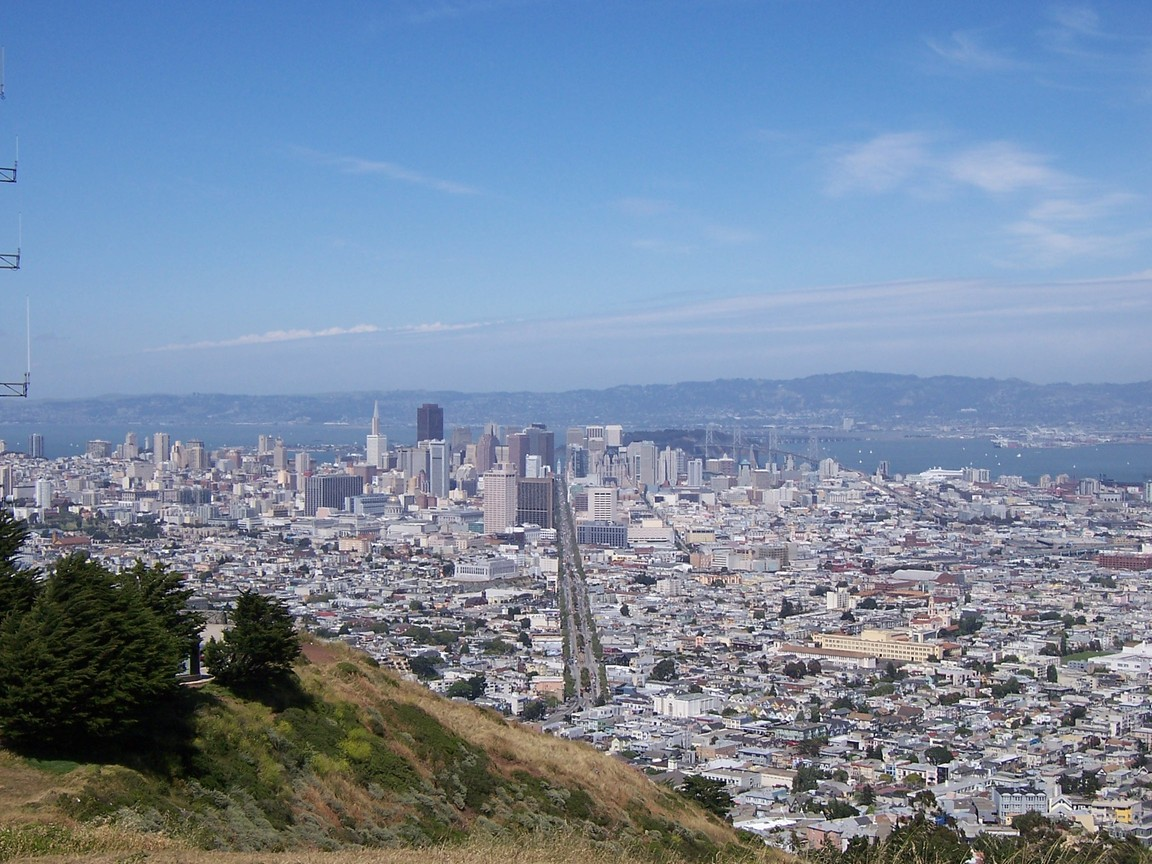
\includegraphics[width=\textwidth]{gfx/100_1168}\end{center}

Our final port of call is Twin Peaks - which really IS the highest point for miles. We soak up some breathtaking views of the Bay and city, spread out beneath us like a Lego playset, from our feet to the watery shore.  While waiting at lights on the road there, a pimped-up car pulls alongside us and brakes to a stop - but what's this?  His hubcaps are spinning away like some kind of crazy optical illusion.  It is our first experience of `spinners'.  We are in awe of his badassness.

We finally managed to secure my Union Jack to the crossbeam of the car, and once we hit the road for good, I cast it up into the air and it unfurls behind us.  It is a picture of majesty and patriotism until it gets caught in a vortex, wraps around and threatens to smother Imran while he's driving at speed through a tunnel.  I rein the wayward flag back in as we cross the Bay Bridge into Oakland - majesty can wait.

\section*{Yosemite National Park}
We pass a good deal of oddballs on the road to Yosemite, some of whom we take pictures of.  We collect images of Puerto-Rican gangsters, annoying children on the back of motorbikes with faces you just want to punch and a huge variety of emetic bumper stickers.  Earlier in the day, when we were packing our bags, we'd had the television on and news anchors were reminding families travelling around (it's Memorial Day weekend - a public holiday) that it is more fuel-efficient to load their roof racks with minimal windward surface area.  We find it difficult to believe that anyone would be stupid enough to attach their coolboxes chunky-side forward on a roofrack instead of smallest-area forward (it's basic wind resistance, right?) but after a few hours on the highway, we begin to realise that elementary physics seem to be beyond some people.

To be fair, we surmise it is a simple by-product of the American manufacturing modus-operandi.  Our theory runs thus:  People load their cars, roof racks, et cetera badly because they just don't notice the difference.  They don't notice the difference because their cars are so powerful and so blockily-shaped in the first place.  The cars are this way because the American manufacturing mantra is essentially ``we can't make it good, so we'll just make it \emph{big}''.  This is why you can tell an American car and a Far Eastern or European car apart in seconds.  Imran and I joke that most of the boxes we see attached to the cars we pass are probably just filled with bricks, because, hell, why not?  We also imagine that the cars themselves rely less on internal combustion and simply work by jetting high-pressure crude oil out of the exhaust and letting Newton's third law do the work.

When it's my turn to drive, we pass an SUV full of guys who are clearly on their way to fun and mischief.  There's an instant understanding between our two vehicles, a connection that only a load of guys on road trips can make, and we spend twenty minutes alternately overtaking one another - only when we pass, a guy in the back winds down his window and sticks a cardboard box out.  With a shock we see what looks like a \emph{head} in the box, before we realise that it's in fact HIS head, and he's taped the box to it and his shoulders.

We laugh as the cardboard-clad nutter starts to headbang, his head in actual danger of blowing away - and we ready our cameras and overtake again, grabbing some quality stills.  With a wave goodbye we zoom off, and secretly hope that maybe they were going to Yosemite too.

As we ascend into the Sierras, we ride past some \emph{real} hillbilly stuff - places where the only radio you can receive is a choice of KGOD, KJESUS-103 and my personal favourite, K-YOU'RE ALL GOING TO BURN IN HELL.  Places where there are more churches than inhabitants, embassies of all colours of the Christianity rainbow, and they're all handily listed on massive boards titled `Places to Worship' as you enter the town.

We wryly note the lack of mosques.

Cedar Lodge is nestled off the road, surrounded by hills and trees, and is very beautiful.  We unpack, grab some dinner at the lodge's really awful 50s-style diner (covered in Elvis stuff - isn't that an anachronism?), chug down some beers and retire.  I watch Wind Talkers on the TV (gritting my teeth as the adverts interrupt every five minutes) and fall asleep to Lostprophets in my new-media-whore earbuds.

\chapter[Yosemite National Park]{Sunday, May 29: Yosemite National Park}
In the morning we dine with the Sierra Shadow Casters, who are a group of leather-clad bikers in the traditional Hells Angels style.  While we are in awe of their obvious coolness and secretly wish we could follow in the ways of whiskey-drinkin' and hard-bikin', frankly we are scared they'd kill us and eat our bodies if we happened to be at the breakfast bar at the same time as them.  We waited until they were done while making smalltalk with the five hundred-year old shrew-like Skeletor woman who, with infinite disdain, agreed to boil us some water since, well, we needed it to make \emph{tea}.

It's true what they say about food in the USA, it's all bigger.  Not the meals themselves, per se, but the actual individual items on your plate. I seriously suspect foul play and/or growth hormones this morning as we chomp through strawberries the size of a human head.  Clearly the `fix-it-with-drugs' ethos so prevalent here extends even to pumping strawberries full of... I dunno, strawberryosterone.

The plan is to get out early and, well... I'm lying.  There \emph{is} no plan.  Even the proto-plan - get to the National Park proper before the rush - flops on its face as we turn out of the lodge and straight into a traffic jam.  Yep - Holiday Season certainly has started.

Our flesh crisps in the sun as we crawl on, following a mighty river flushed with melting snow from the nether regions of the mountains, and into the Park.  We hand over some money at the gate for a ticket and a guidebook.  The book suggests we start off by climbing straight up to the highest part - Glacier Point - and soaking up the view before maybe following one of the numerous trails on foot.  It sounds good to us and so we begin to ascend.

At about 6,000ft we begin to suspect that `Glacier Point' is named not for what you can see from the top but for the fact that it is quite literally atop a glacier.  The lush forest and streams quickly give way to ice, frozen tundra and channels filled with the roaring of liquid pouring from the melting snow heaps.  It is very \emph{cold}.

The gruelling climb began to take its toll and it doesn't take long for our fuel gauge to dip into the region I call `oh shit'.  I began to panic and soon start suggesting courses of action like putting it in neutral and coasting back down to sea level.

Nevertheless, at an altitude of eight thousand feet, the road ends and we pick out a space in the brimming car park.  Bundling out and wandering to the scenic overlook, we meet the most awe-inspiring sight yet: one hundred and fifty degrees of Yosemite National Park (with the remaining degrees of the panorama blocked by, well, a \emph{mountain}).

It was enough - over there is Half-Dome and, uuh, some more peaks, and some valleys, and - well, they should have sent a poet.  Despite the altitude sickness, my inner ear sloshing uncomfortably and the mass of holidaying families, I commune with nature and marvelled at the forces that could create such beauty (no, not \$DEITY, \emph{glaciers}).  It is unreal; I want to reach out and grab it to make sure it isn't a painting.

\begin{center}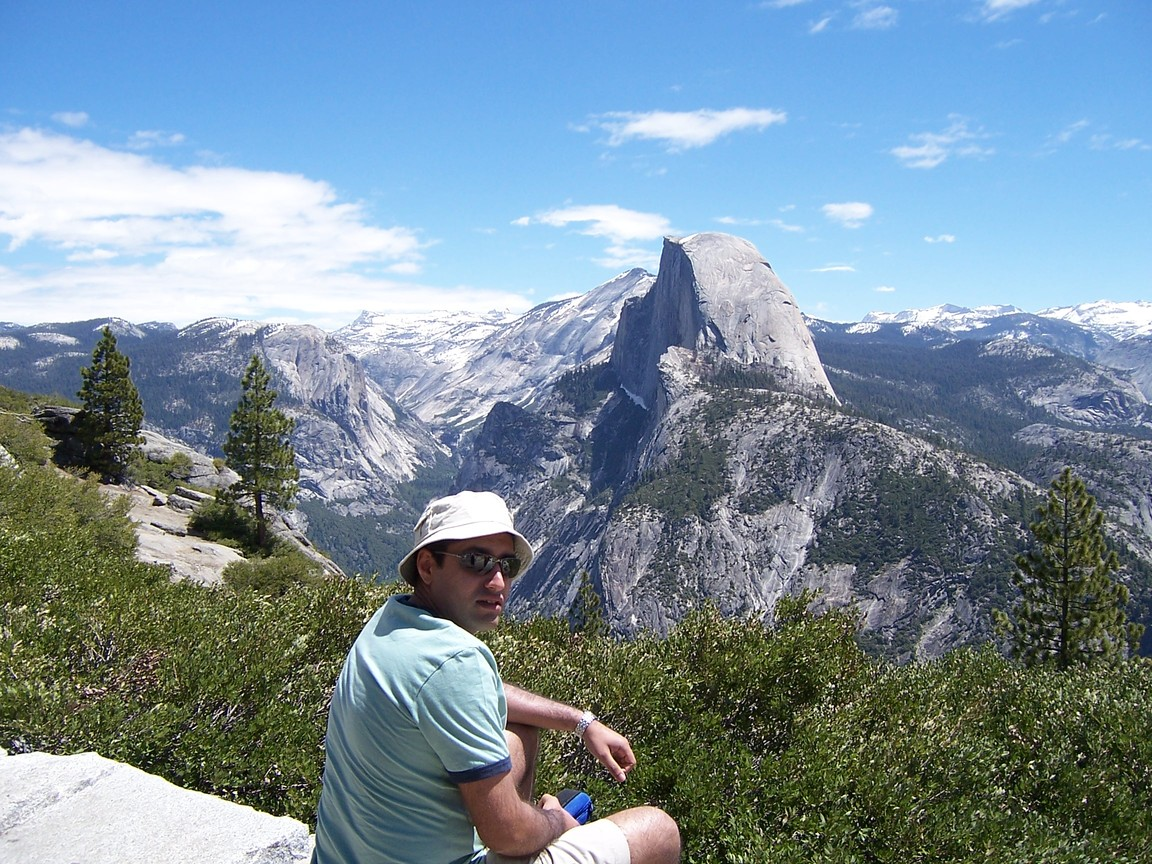
\includegraphics[width=0.8\textwidth]{gfx/100_1213}\end{center}

There is a visitors' centre, gift shop and caf\'{e} here; we're a little hungry and so we grab some trail mix and a `powerbar' - basically an emetic slab of frozen peanut butter - before realising that we'd screwed up.  We \emph{should} have parked the car at the bottom of the park, got a free shuttle up and then hiked down.  What we had to do now was drive all the way back down and miss out, because by the time we got back to base camp, the free shuttles will have stopped for the day.

We realise that there's little else we can do with a near-empty tank of gas and so we leave the park in search of a fill-up.  Thankfully, due to the enormous amount of traffic and correspondingly slow speeds, we get out with gas to spare and manage to pick our way to the nearest dot on our map, a hamlet called El Portal.  It is tremendously `backwater'.  My erstwhile colleague correctly declares that ``this is some Chainsaw Massacre shit.''

We only just manage to fill up with gas before being skinned and eaten and decide to brave the traffic once more in order to see some more of the park from ground level and check out El Capitan.  El Capitan is an impressive, giant monolith which, I'm sad to say, excited me more by virtue of its upstaging of Shatner in \emph{Star Trek V: The Final Frontier}.

\begin{center}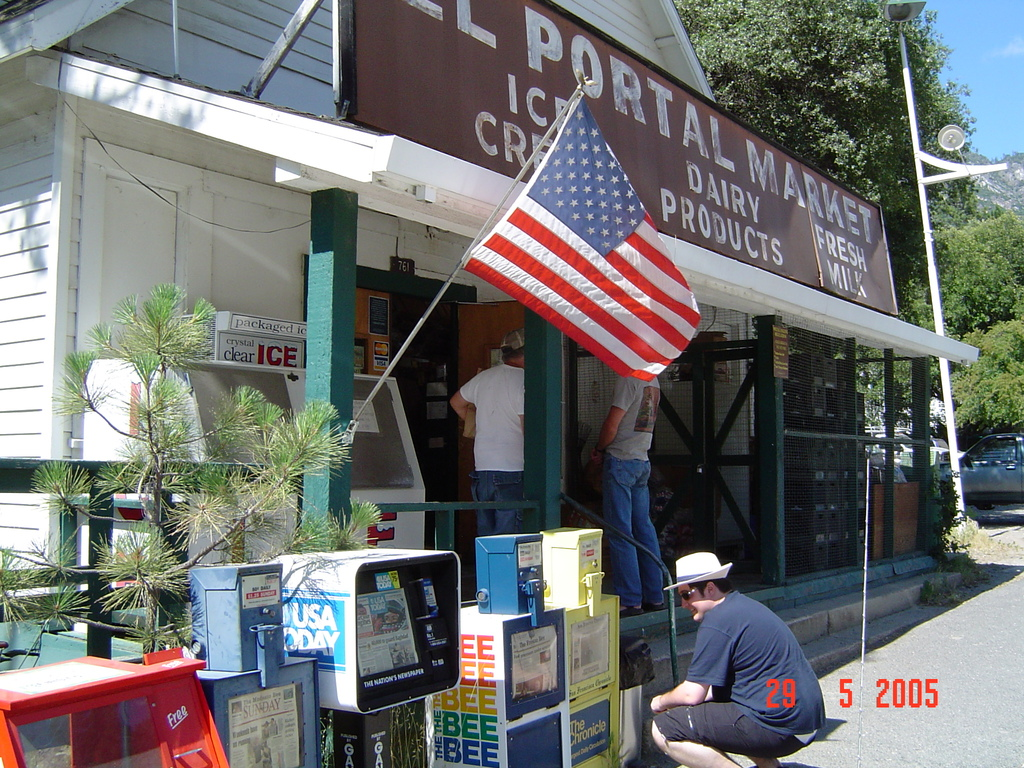
\includegraphics[width=0.8\textwidth]{gfx/DSC00663}\end{center}

By the time we find a place to park and start hitting the trails for a walk, though, it is getting dark and we are forced to abandon our plan to find and wrestle bears.  Instead, we plump for a much shorter route - a route which still had us panting and sweating like Michael Jackson at a school play.  Finally we reach the end and reward ourselves by hanging out on a bridge close to a small waterfall, lapping up the spray and absorbing Nature's glory.

In lieu of the long drive we had planned for the next morning, we decided to take it easy that evening and plan the route over a beer back at the Lodge.

While we arrange our checkout, some wise old man sitting at the souvenirs desk overhears our plans and, in a true hillbilly \emph{I'm gonna take advantage of your naivety and kill you with a chainsaw} moment, looks us over and whispers ``you boys heading to Vegas? I got some \emph{baaaad} news for you''.  Thankfully he wasn't going to cut us up and eat us, but informs us that the Tioga Pass - our route over the Sierras - is \emph{still} knee-deep in snow.  We would have to find another way into Nevada.

``The pass is only closed in winter'', I protest.  ``It's almost June!''

``Things don't always go to plan out here'', he rasps.

Our re-navigation has scuppered Imran's desire to forgo the route Virgin had planned for us and burn our way across Death Valley, for which I am secretly thankful - the very idea of straying from the plan scares the crap out of me.  Instead of crossing the mountains, we'd have to follow them south in a massive detour through Fresno and Bakersfield before turning east, skirting around their tip and heading up into Nevada the \emph{long} way around.

It was by all accounts going to be a colossal journey and so we pack up our bags and hit our respective sacks.

\chapter[Yosemite -- Las Vegas]{Monday, May 30: Yosemite -- Las Vegas}
Our road takes us through the Californian central valley, the slow decent from the heights of Yosemite taking us past some beautiful countryside including the alien sights of orange groves.  It was my turn to drive; we'd divided up driving duty such that I did the long easy roads and Imran did the urban areas - ostensibly because it had been a few years since I'd owned a car and was therefore a little rusty.  The real reason was, of course, twofold: driving on single-carriageway desert highways disappearing to the vanishing point was my ultimate reason for being, and I was completely paralytic with fear of the idea of driving around the megalopoli we were hurtling towards.

We decided we could spare a few minutes and left our busy highway to duck into a small road lined with orange trees.  It was a road that went to nowhere and we shouldn't have been on it, but the road epitomised everything we were looking for - despite being only half a mile from the busy main route, it was deserted, flat and perfectly straight, the shimmering tarmac rushing on to its date with the horizon.

We absorb it for a few minutes and rejoin the throng.

\begin{center}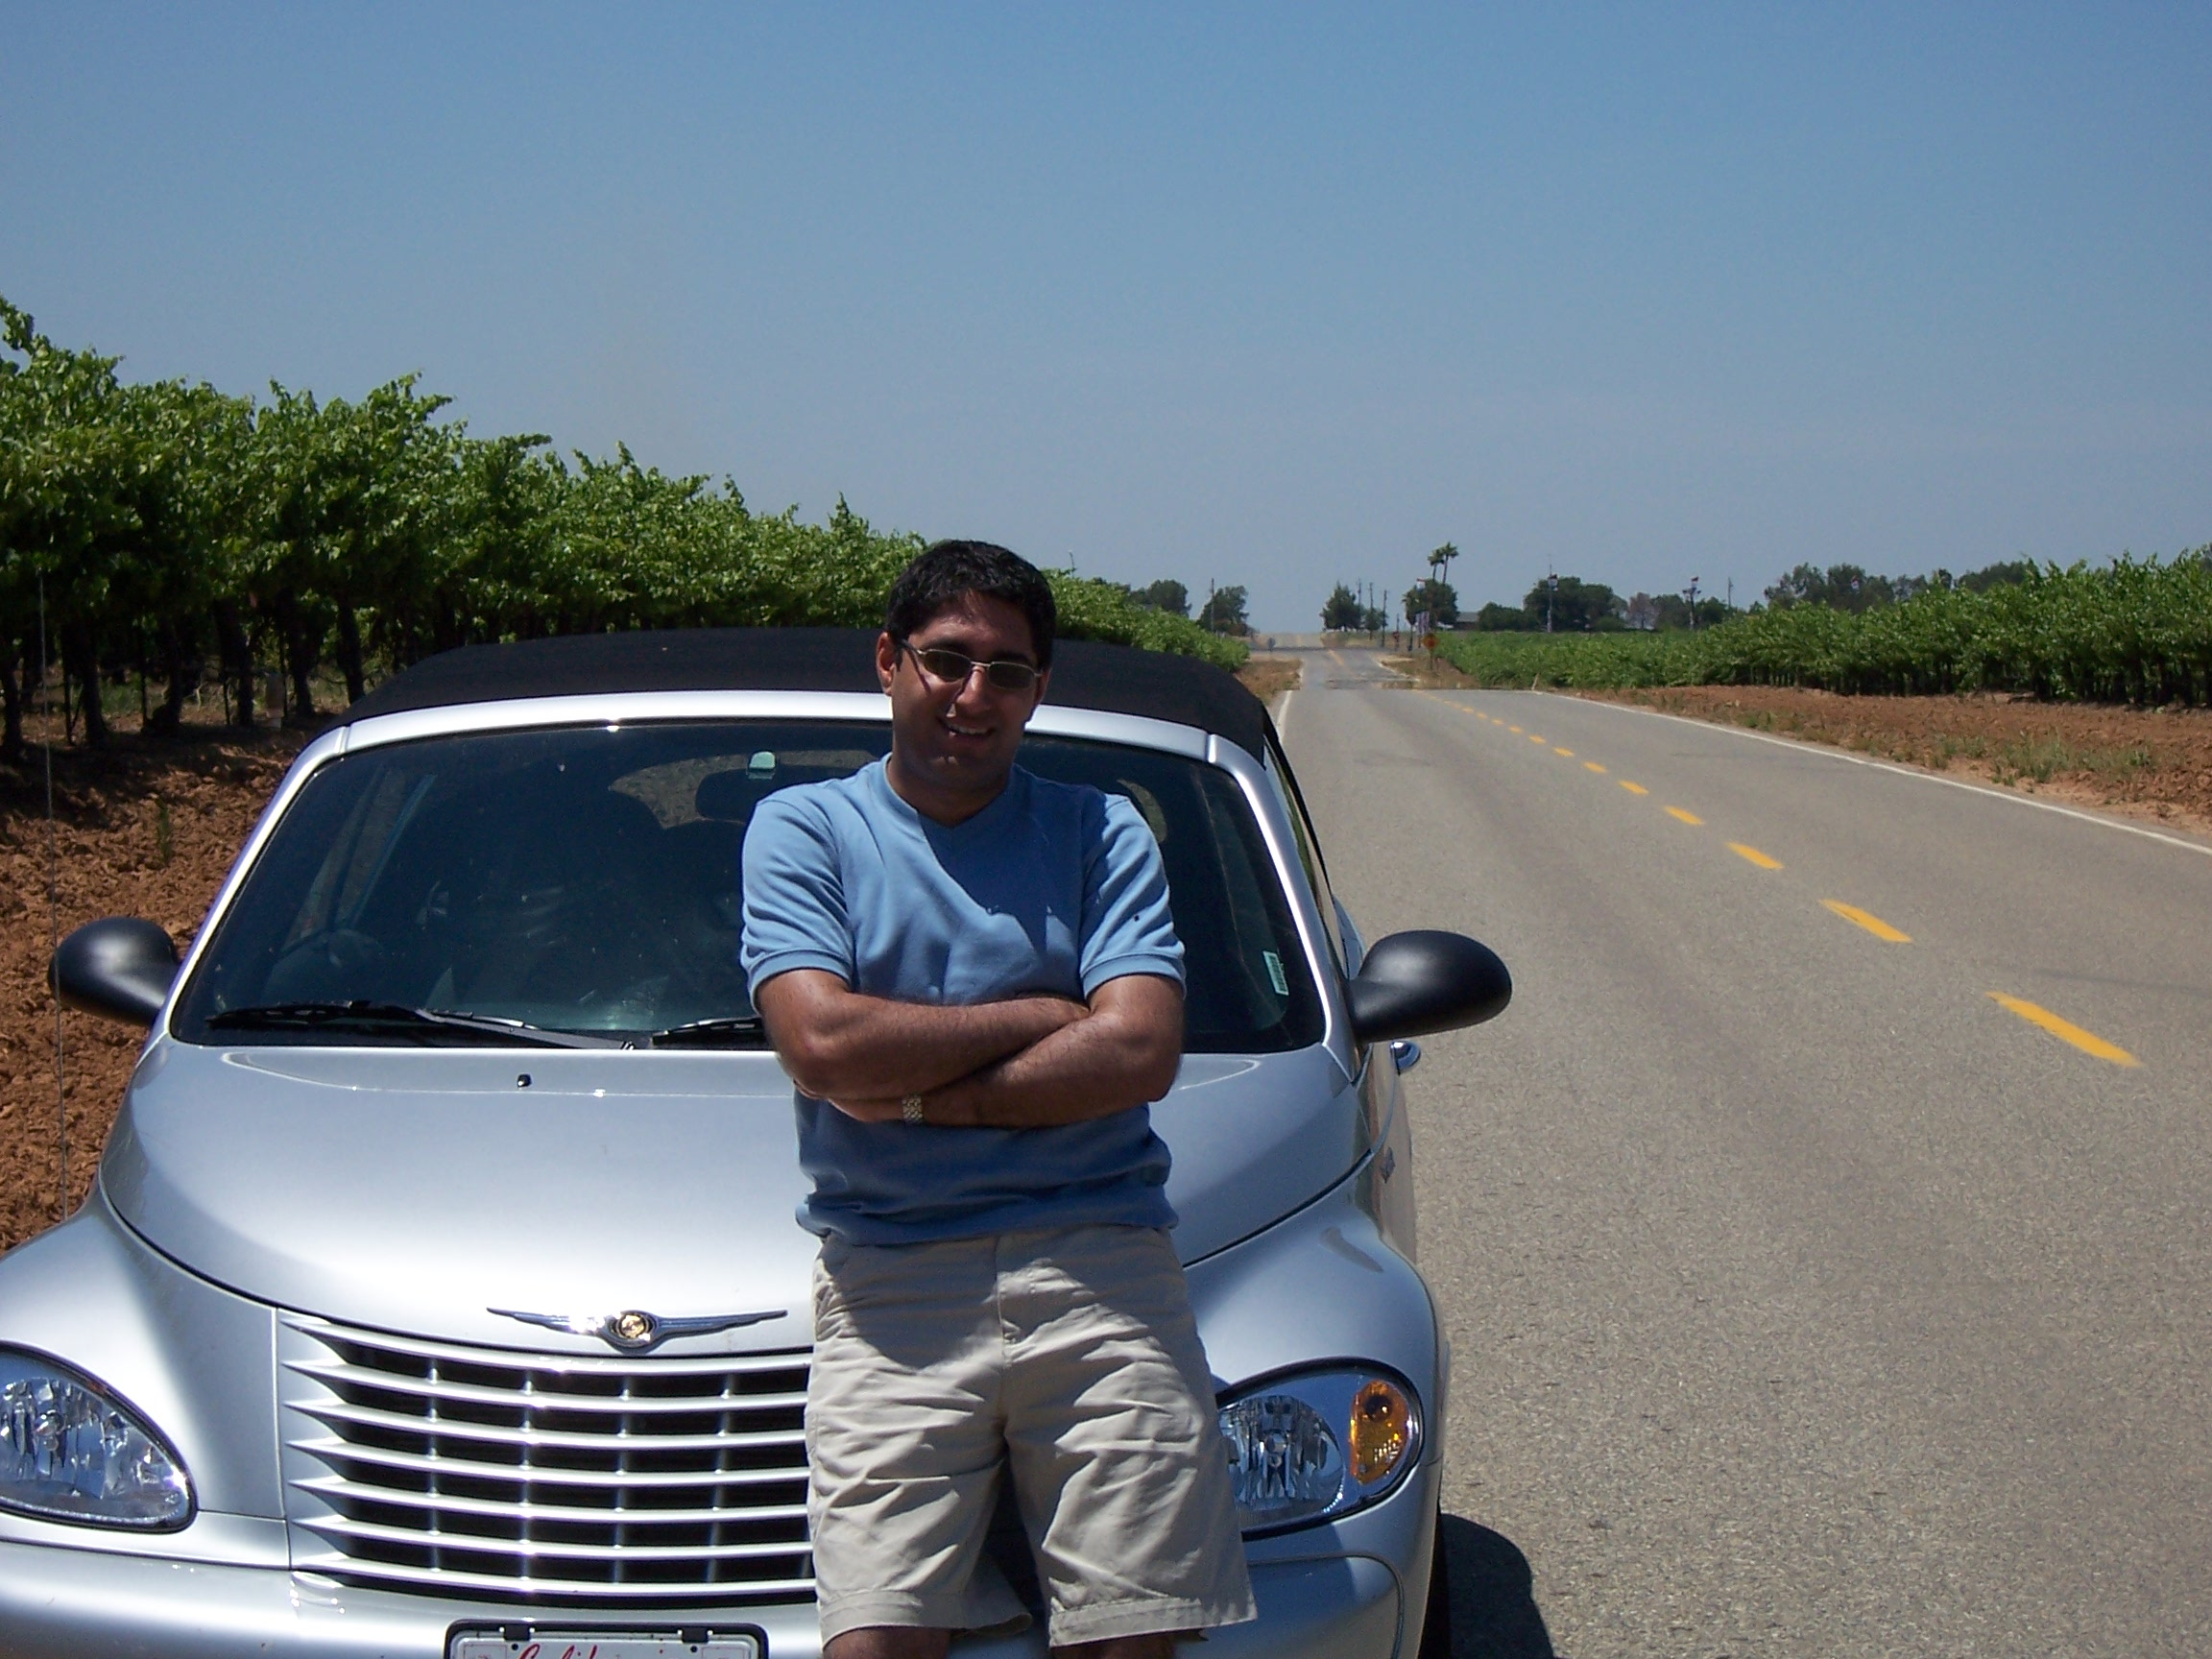
\includegraphics[width=\textwidth]{gfx/100_1307}\end{center}

Past Fresno we park at a truck stop for a quick bite and order quesadillas from the bored Mexican man-child at the counter.  They ooze with grease as we wolf them down before filling our tank with gas and resuming our pilgrimage.  We pass billboard after billboard after bumper sticker reminding us - lest we forget - that \emph{Jesus is Lord}.  It seems that, in this foreign land, they really take this sort of thing seriously.

Hours pass.

At Bakersfield, Imran's desire to abandon the route we had been given and, instead, head into Death Valley finally triumphs over my own, more conservative desire to reach Las Vegas alive.  Besides, he argues, the route we are following takes us way too close to Los Angeles.  In a way, it feels like cheating - we both agree that we don't want to come close to our final destination until we are actually \emph{supposed} to be going there.

When the moment of truth comes, the point of no return, we turn off the main road and head into the desert.

\section*{Death Valley}
\begin{center}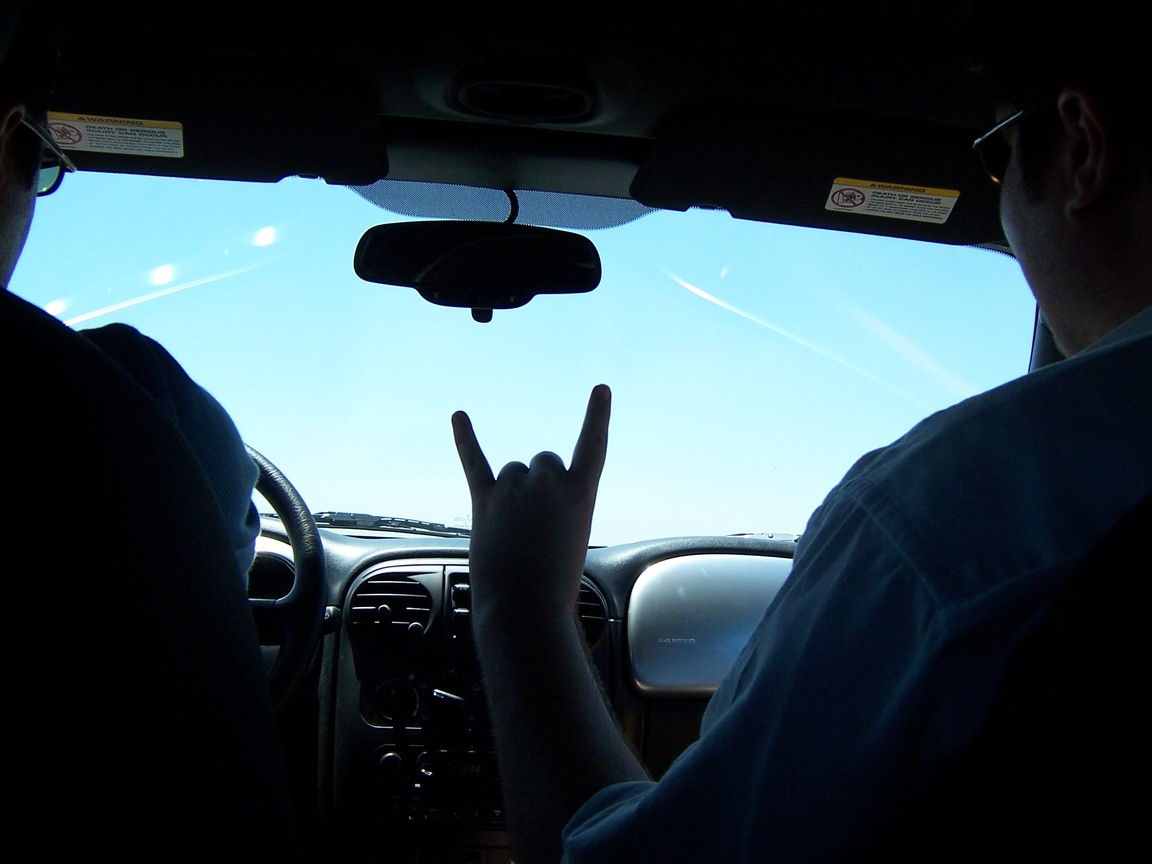
\includegraphics[width=\textwidth]{gfx/100_1298}\end{center}
If we were going to do it, I wanted to do it with a car full of provisions and fuel (you can't be too careful) and so our first stop was California City (or the town of Mojave, since I'm not sure that California City isn't just a crossroads in the middle of nowhere).  Mojave is, of course, now famous for its eponymous Space Port and the home of Burt Rutan's SpaceShipOne - when we arrived it was famous for being dusty, hot and choked with traffic so much so that I lost my temper and, after finally pulling in to the gas station, insisted that Imran should drive.

The gas stations at Mojave kindly provide all sorts of tools and supplies to clean your windscreens of desert dust and dead bugs; we make good use of them after buying many bags of jelly babies.  We would later come to regret our choice of dinner or, at least, our decision to travel without indigestion tablets.

As we turn north-east and headed out into what I've always wanted to believe was my spiritual home, the Mojave Desert, we began to realise that, once again, we'd fallen prey to the Scale Spaz.  As it happens, the distance to Las Vegas through Death Valley is about the same as your average trip to the Moon, and before long the signs of civilisation begin to wane.  The trees and orchards began to give way to scrubland and bush and the temperature climbs with every mile we advanced.

Taking in the big open sky and long, straight, baking hot road we cruise along with nary a road user in sight.  Wind farms begin to spring up on the hillsides, giant turbines in huge quantities, and that reminds me of something I'd always wanted to do:  Now that I was out of the driving seat and free to relax, I insisted we play one of my most favourite albums of all time, Kyuss' \emph{Sky Valley}, a record which was made \emph{by} desert creatures \emph{for} desert creatures.  Of course, anyone worth their salt would know that I was in the wrong area for Kyuss - Palm Desert, their home, is a great deal further south than us - but at the time I didn't know it, and it didn't matter.

Nature called and we pull off to a road heading south.  After driving sufficiently far to avoid prying eyes we see a railway crossing and, slightly before the crossing, a train. I suppose this shouldn't have been a surprise, but this train seemed be modern, fully loaded, hugely long - and utterly abandoned.  Imran and I, eager to snap up some pictures of the slithering beast rolling on past us, sit and wait for it to steam on by but it steadfastly refuses to move.

It is \emph{eerie}.  It is as if the train is waiting for the crossing to clear (it \emph{was} clear - we are the only traffic in all directions and we are wholly stationary) but the driver had just decided to go to pop out for some groceries or something.  Except of course there's not a living soul (not even a Walmart) for miles around.  We find it fascinating and even mildly scary - something that just shouldn't \emph{be}.  We get as close as we dare, play on the tracks like children, and take pictures.

\begin{center}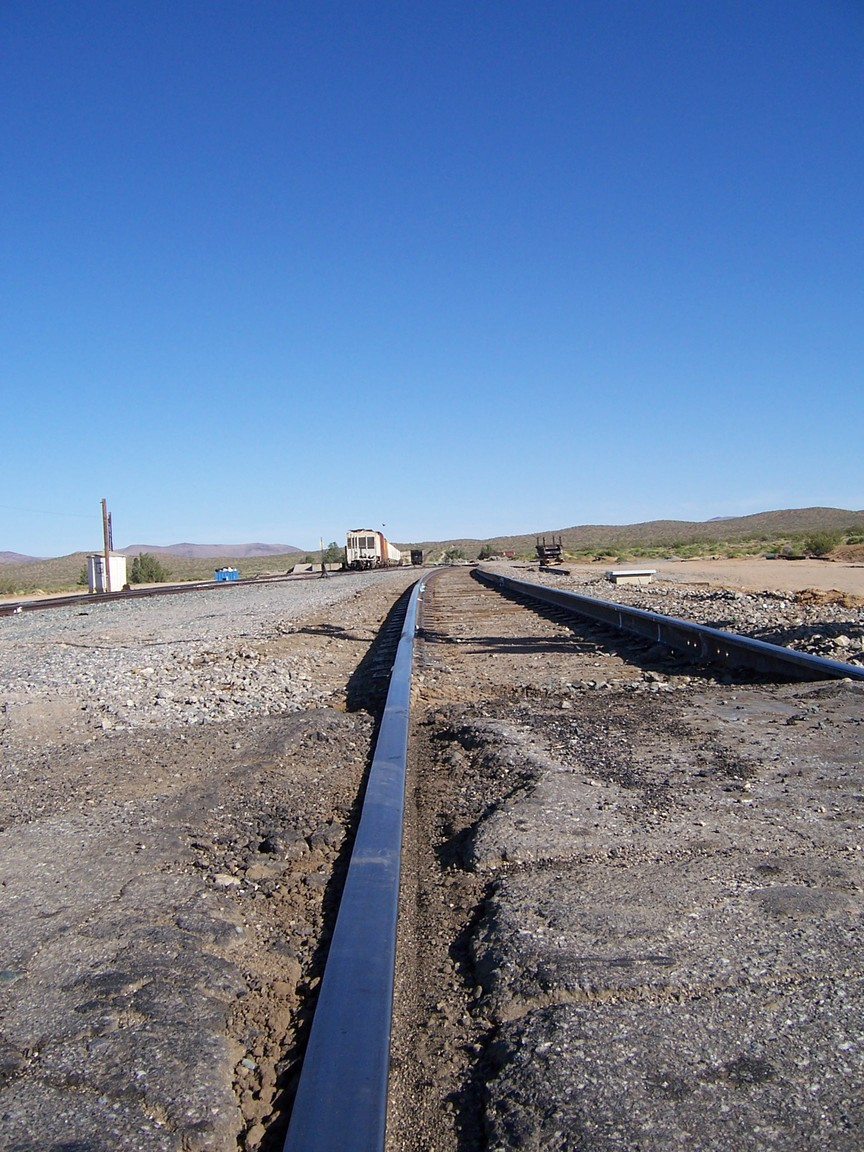
\includegraphics[height=100mm]{gfx/100_1346}\end{center}

Onwards, then, norther and easter, until the vegetation begins to fail and we reach China Lake, a dry lake and also the home of the China Lake Naval Weapons Center.  Naturally we are slightly concerned with the idea of being a stone's through away from, I dunno, instant fiery death from a wayward Naval Weapon and so we urge the car forwards with gusto, skirting its eastern border and heading almost due north into yet another dry, salty basin - Searles Lake.  Searles Lake is surrounded by chemical works of some description and really is a perfect candidate for that most peculiar tradition of naming settlements for their primary export (like Borax Springs, CA or Chloride, AZ or Molybdenum, KS (I made the last one up)).  Of course after a few more miles we found out they had done just that - hello, \emph{Trona, California}.

We start to climb and pass beautiful natural landmarks - like a discarded bag of fast-food leftovers - until we had cleared our hill and see, spread before us, the Panamint range - the western walls of Death Valley.  We stop the car and breathe it in: Telescope Peak, the highest point in the National Park, away to our right, the still-blue (but rapidly darkening) sky, the valley floor itself spectacularly arid and empty and, ahead, our road down into the Panamint valley and up again, heading east to the Park and beyond to Nevada.

Our (well, fine, Imran's) plan is to avoid main roads as much as possible and essentially creep into the valley by the back way.  This we achieve with distinction, only using the main route when it is absolutely necessary and leaving it again at the first opportunity.  With only a (admittedly comprehensive) AA Road Map I'd bought back home, this is tough going and, as dusk falls and the fuel gauge hits the wrong side of the quarter mark, I quietly panic about the possibility of being stranded in Death Valley.  Let's face it, if it was called `Happy Friendly Valley' I might have felt a little better but it was baking hot still; even at eight PM it was \emph{thirty-seven degrees} inside the car - it being a convertible and us being low on gas I veto air conditioning.

We climb the Panamint range and, at its peak, decide to explore what looks like an abandoned missile silo or nuclear bunker.  We fantasise about sitting out Nuclear War here, and that there is probably an entire city underneath our feet but, in the end, we think it prudent to carry on down to the Purgatorial valley floor.  Past Stovepipe Wells, Beatty Junction and the road snakes out ahead - not another car to be seen, so we put pedal to the metal.  Despite mild panic about our fuel consumption, we feel exhilarated as we power through the hot desert air at speed, past mountainous sand dunes looking wholly out-of-place this side of a beach; top down and music loud.  There is an upturned, abandoned sofa on the side of the road.  We wonder who on Earth travels to Death Valley and throws a sofa away.  Signs point to places ahead of us, Furnace Creek; Badwater (the lowest point on the entire continent).  It is pitch black.

Soon we reach the `tourist hub' of the National Park, Furnace Creek.  It is deserted but there is, finally, a self-service gas station - I could cry with joy, but lose the game of rock, paper, scissors and so I am the one who must fill up the car - surrounded by empty darkness, fearing that `anything could happen out here'.  I fill up, \emph{quickly}, while Imran keeps alert and ready to flee in case there are, well, hillbilly murderers.

We make Furnace Creek eat our dust and fly east, deliberately keeping up the eerie tension by imagining zombies and killers around every turn - until we see a human step out on to the road in front of us.

Imran slams the brakes on and we screech to a halt in front of a man, standing alone, his hand out as if to ward us off.  We look at each other and whisper `fuuuuuuuuucccck!'.  Imran keeps his foot a mere atom's width from the accelerator.  We are ready to fight for our lives.  The man is surprisingly dressed for a murderer, he is wearing a high-visibility reflective jacket and his murder weapon is a long `Stop' sign.  His name is Chris.

Chris tells us that there are some roadworks ahead and we must wait with him for an `escort car'.  He's a clever one.  We don't trust him.  He radios an associate and tells him to `bring the truck'.  The Zed and Maynard scene from \emph{Pulp Fiction} plays through our heads and we share a nervous glance.  He tries to make smalltalk but we're not in the mood; Imran turns the radio on to cut him off.  We wait for him to strike.  He bides his time.

Eventually a truck arrives.  Chris and the driver have a chat.  The truck turns around and, on its back, there is a sign saying `Follow Me'.  We follow it.  Chris waves goodbye and hopes we enjoy Las Vegas.  We had escaped... but \emph{for how long?}

\begin{center}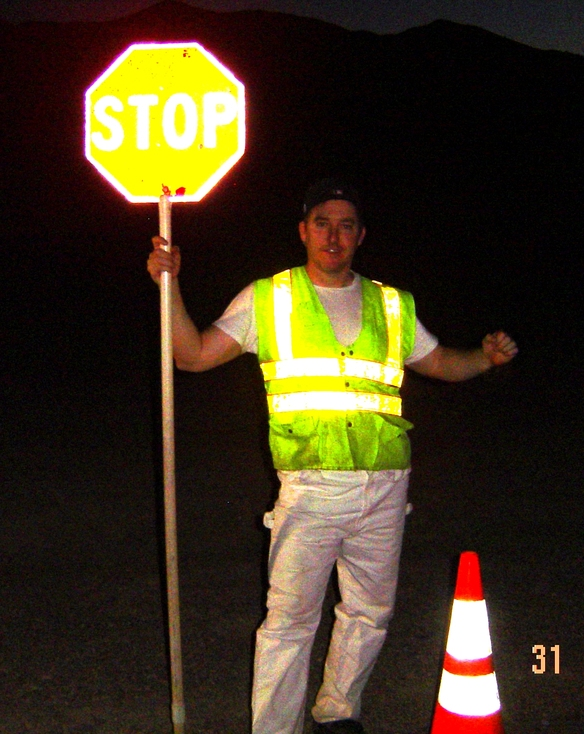
\includegraphics[height=60mm]{gfx/DSC00683}\end{center}

Death Valley Junction and, somewhere in the darkness, we cross the state line into Nevada.  I lament not being able to get a picture of the sign informing us of this (there may not even have been one) but have to focus on the more important issue of `where the heck are we'.  It is now very late and, having left the heat behind, the chill begins to set in.  We apply more gas and hurtle through the night.

Eventually, up ahead, bright neon lights begin to rise from the horizon.  We grow excited - could this be Sin City, rising to meet us?  There are signs and hustle and bustle galore as we near the city limits, casinos and motels, a welcome change from the day's desolation - but what's this?  ``Welcome to Pahrump, NV''?!  It's not Las Vegas.  It's some horrific copycat city between it and us.  Close-up, it looks downtrodden.  Depressing.  We feel a little sorry for it.

We step on the gas.

\section*{Las Vegas}
Fuel crisis averted, I now begin to panic that for some reason, the hotel won't let us check in because it's too late at night.  We would have to sleep in the car.  On Las Vegas Boulevard.  This won't do.  A line of hills rises up and comes towards us - Mountain Springs.  We climb it, reach the top; the nose of the car tilts down a little - and there it is.  Las Vegas fills the floor of the great basin ahead of us with light.  Innumerable lights and, in the midst of them all, a great spike of light pierces the sky - of course it's the light atop the Luxor, a beacon drawing everyone's gaze to the Strip (which, as any pedant knows, isn't actually in Las Vegas proper).

It is spellbinding.

Route 160, across the Las Vegas Freeway, and onto the Boulevard.  We turn north and head up.  We're staying in Mandalay Bay at the extreme southern edge of the strip itself and I insist we head straight there rather than prowl up and down the strip itself (a decision I'd later regret, everyone should take every opportunity to drive the Strip at night).  We pass the iconic `Welcome to Las Vegas' sign and high-five with glee, before turning left and crossing to the front of the Hotel, standing majestic, golden and tall, immediately south of the Luxor's pyramid and searchlight.

There is a little confusion since the signs outside say `Four Seasons' rather than Mandalay Bay, but in our delirium we ignore that; according to the map and signs, we're in the correct place.  Imran is impressed - apparently Four Seasons is quite posh, perhaps `Mandalay Bay' is simply a franchisee of some sort.  A valet asks if he can take our luggage and we agree, privately agreeing not to tip him.  With infinite bravado we approach the front desk and ask to check in.

We're not on their system.  We have no reservation.

Impossible - we show the clerk our booking vouchers.

The clerk points to the part of the vouchers that say ``Mandalay Bay''.  He then points to the sign behind him that says ``Four Seasons''.  We point to the map and road signs.

Ah yes, he says.  The Four Seasons, although physically attached to the Mandalay Bay, is an entirely separate enterprise, and we must pack our stuff up, leave, turn around and go around the `back' way.  We are most certainly in the wrong hotel.

We recover our baggage from the bemused valet, fail to tip him for bringing them ten metres, walk right back out of the door, pack our stuff up, leave, turn around and drive up the strangely thin and winding `back' way.

A new valet whisks our car away; it's the first time I've had to deal with this concept and I have to admit I don't really like it - would we have to pay every time we parked?  It seemed like a bit of a pain.

I am soon soothed by the luscious interior of the hotel.  Of course there's really no such thing as being `too late to check in', \emph{especially} in Las Vegas, and within moments we are enjoying the spacious, decadent, air-conditioned lobby and taking the elevator up to our spacious, decadent air-conditioned room.  We were very high up, facing south - away from the city, with a wonderful view over the airport and badlands beyond.  There is an almost comical contrast with the view directly beneath our window, that of a tropical watery wonderland (it's Mandalay Bay, after all) complete with pools, wave machines and sprinklers - a fantastic display disregard for our arid surroundings.

We were filthy and tired but there was no way we were going to turn in without first having a look at the casino floor.  After a freshen up and a change of clothes, we headed down to check it out.  Once past the tacky gift shop, there is an ocean of slot machines; beyond the slot machines there are the tables - blackjack and roulette of course, as well as some esoteric ones that apparently are Big In China.  Beyond the tables are the game rooms and next to the game rooms is the crazy Sports Book section, with its wall of video monitors and easy chairs.  The air is fresh and cool, the place is clean and modern - it is our first glimpse of a `real' casino and we're impressed.

Alas, this being our first time, we are way too meek to even attempt any `real' gambling.  We are worried that we might do something wrong and end up in a back alley being violently beaten by large security guards (looking back on it we can admit this is somewhat unrealistic); we don't know where to get chips from - we don't even know if it's \emph{okay} to just wander up to a roulette table and do our thing.  Is there a queue?  Would the other guests frown on us?.  We are also terrified of the minimum bets - five dollars?!  Forget it!

In the end, we decide to pointlessly and fruitlessly waste a few moments on some slot machines before turning in.  I am so exhausted I fall asleep in my clothes and, sick with what we've decided to call `desert fever', we both have a restless and unsatisfying night.

\chapter[Las Vegas]{Tuesday, May 31: Las Vegas}
We awake feeling incredibly dehydrated.  The industrial-strength air conditioning of the hotel has sucked the moisture from our bodies; it's a small price to pay for such blessed chilly comfort.  We decide to break our fast in one of the hotel restaurants.

I have smoked salmon bagels for the first time and decide they are the best thing since sliced bread.  After filling up we decide to investigate our immediate surroundings - the hotel.  It's \emph{big}.  It takes us half an hour to get from one end to the other and there even seems to be a fully-equipped zoological aquarium or shark exhibit or \emph{something} at the far end.  We have no real interest in such things (and especially since it seems to cost an inordinate amount of cash) and so we return to the casino proper.

We arrive just in time to catch the croupier's shift change and an incredible earful of profanity from one of the early-morning gamblers at a roulette table we were slowly trying to build up enough courage to sit down at.  He's clearly been there all night and he clearly wasn't winning.  He calls the croupier a funking motherhubbard; the croupier washes his hands of us and leaves.  We're enthralled.

Our courage fails and we retreat to some slot machines.  I try to get to grip with that most pervasive of games, Video Poker - I've never played \emph{real} poker before but somehow manage to fluke my way into winning one dollar twenty five cents.  I hold my first winnings voucher close to my heart and vow never to cash it in, indeed, to frame it.

Imran, still suffering from Desert Fever, decides to have an afternoon siesta and retires back to bed.  I decide it's high time I hit the strip.

\begin{center}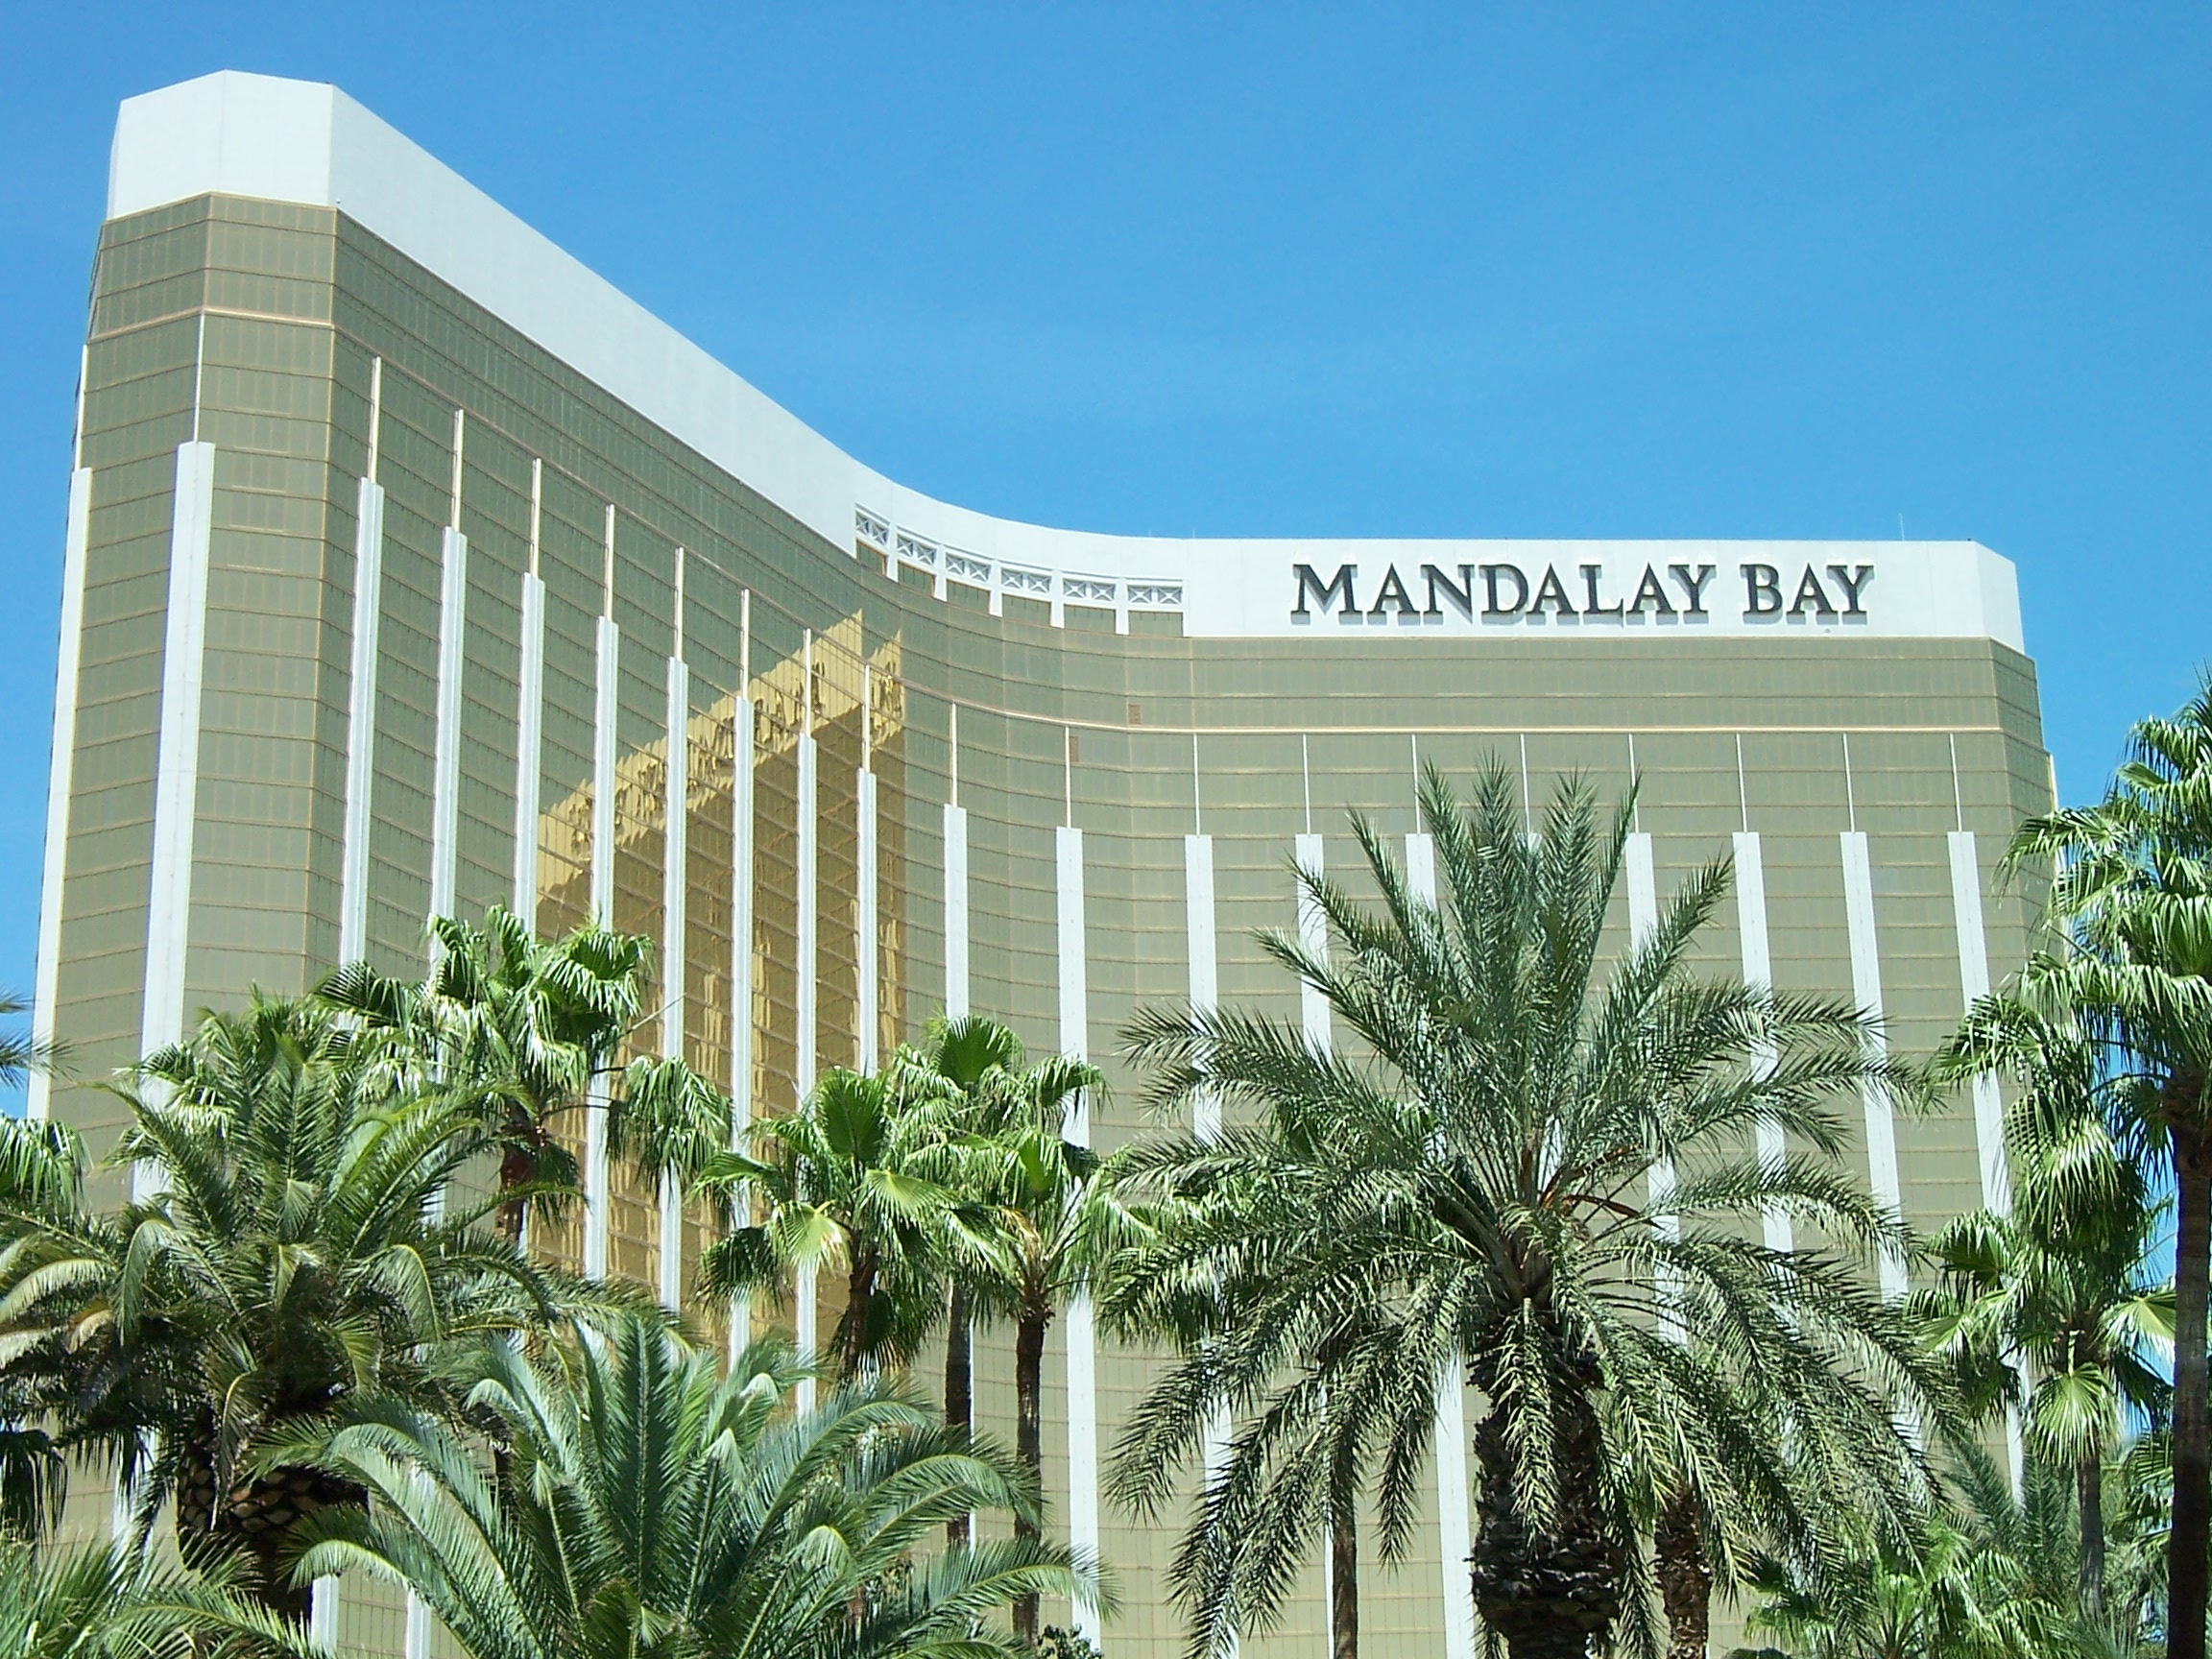
\includegraphics[width=\textwidth]{gfx/100_1388}\end{center}

Leaving Mandalay Bay I turn left - north - and begin my magical journey.  Luxor is on my left, its black edifice shimmering in the sunlight, every bit as magnificent as last night.  After that - Excalibur, all towers and parapets but looking unfortunately under-dressed compared to its neighbour: New York, New York - a bewildering construction.  My mind boggles as I try to figure out exactly which parts are hotel rooms that people stay in and which parts are simple fabrications for the cityscape.  The famous roller-coaster trundles up and down, in and out.

I cross the Boulevard's six lanes - groaning with traffic even at midday on a Tuesday - to the eastern edge and continue up. Here the buildings take on a more traditional look; the Tropicana, MGM Grand (and its bonkers roomie, `M \& M World'.  I crossed the road again, taking pictures up and down the strip, every bit the tourist.  I was baking hot and \emph{deeply} regretting my decision to wear black and go on a walkabout at midday \emph{in the desert}.  Eventually I sought refuge underneath the Aladdin (now Planet Hollywood) just short of the utterly ridiculous scale model of the Eiffel Tower in front of `Paris'.

I found myself in the Desert Passage Mall beneath the casino (now `Miracle Mile Shops') - it was cool and dark and its decor was wonderful, faux-Middle Eastern complete with cobblestone paths and even an alarmingly convincing skybox covering the ceiling.  I wandered the streets for a little while before finding myself staring lustfully into a rather expensive looking hat emporium called \emph{Hattitude}.

Now, as has been documented, I have an odd predilection for hats.  On my last trip abroad I'd bought a wonderful white floppy paper fedora from, um, Tie Rack or Accessorise or something; I was very much attached to it and had many months of sterling service from it, but it had mysteriously vanished a few weeks before I left.  Distraught at the idea of being abroad with my head uncovered, I'd bought a white cotton fedora just for this trip but it really hadn't been working out for me; it was uncomfortable and \emph{deeply} uncool.  In front of me, however, in this shop, was a fantastic straw hat of quality and fashion.

I wanted it.  I wanted it, but couldn't be sure it wasn't for, well, women.  Having no fashion sense myself, I rely on others to tell me when I really can't wear something - but this time I'm left with little choice but to ask the shopkeepers, a couple of snooty ladies.  My opening gambit is a straight-to-the-point double-whammy of ``does this make me look cool?  Are you sure this isn't for women?''  Of course, seeing nothing but an easy forty dollars, the ladies all quickly agree that yes, I did look cool and no, it really wasn't a gender-specific item.

I bought it and coveted it.  Made in Mexico. I take this as a mark of high quality and am pleased as punch.

I deem it high time Imran joined me and so I leave the underground warren, don my (sun protection guaranteed) hat and head south back to the hotel.

\begin{center}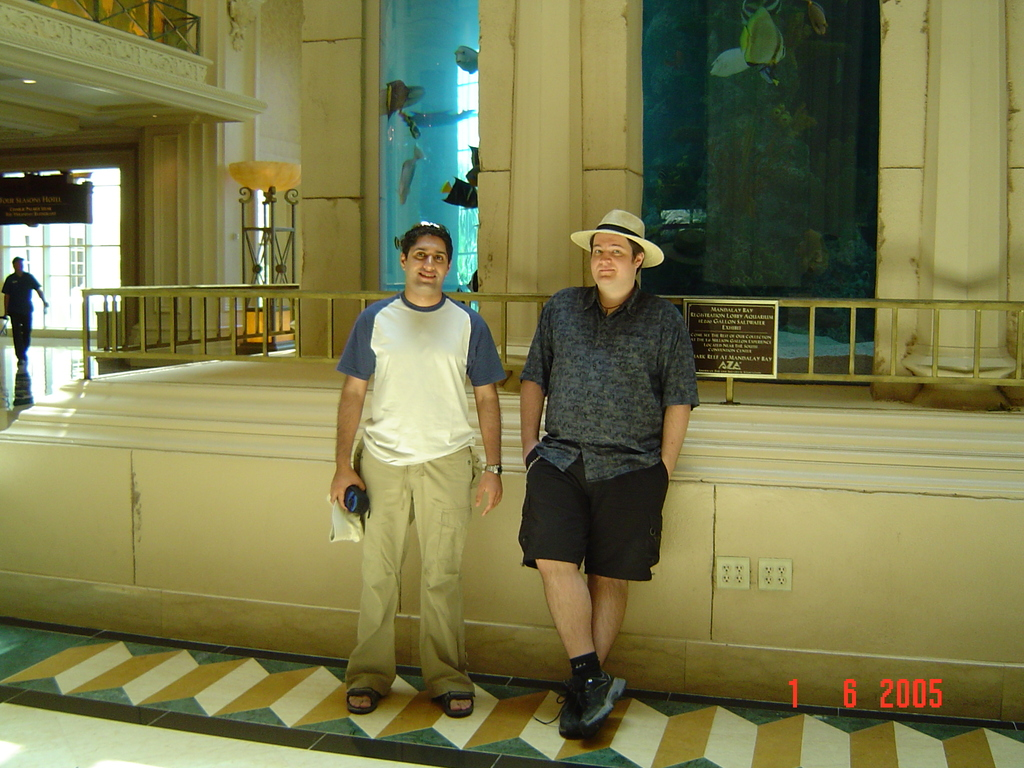
\includegraphics[width=\textwidth]{gfx/DSC00685}\end{center}

After a swift change of clothes I repeat the walk but this time with my erstwhile partner in crime in tow.  We marvel at the sights, the sounds, the people - and always the ever-present heat beating down on us.  We find a restaurant in the Desert Passage and eat a wonderful lunch - but then we make a critical mistake.

We didn't tip the waiter enough.

He hadn't really done a very good job and, hell, we wanted to save our cash so that we could pointlessly throw it away gambling later.  It's a rule I've always lived by - tip according to the quality of service received - but (of course) it's not a rule our colonial cousins appreciate and this was made \emph{very} clear to us on the waiter's face and attitude as he uttered various voodoo curses under his breath and vowed to kill our firstborn.

Deeply shamed, we stuff some more notes under our plates and leg it.

We head out of the mall and decide it's time for us to finally start wasting money \emph{properly} by entering the nearest casino and heading to the game floor.  Since I've come to the conclusion that the slot machines are completely pointless and that there is no entertainment or drama to be gotten from them at all, we waltz right past them.  There are poker rooms, the idea of which I find very sexy but, alas, I don't actually know how to play poker, so they're right out.  There are blackjack tables but I'm incredibly worried that I cannot do the simple mathematics required on demand and the idea of the game `pausing' while I frantically try to sum the value of my cards while everyone watches fills me with cold dread.  This leaves me with one alternative - roulette. 

I'm still too chicken to try it, though, and Imran, growing impatient, decides that the best way to look cool is to start on the blackjack table.  He dives in and I stand and watch, shaking with adrenaline.  He looks So Cool.

Roulette looks easy.  I lurk for a good long time, watching punters `play', and I'm pleased when it transpires there's actually no skill involved at all.  There also looks to be an `easy mode', where people not hardcore enough to want to bet on single numbers or any of the baffling array of rows or columns or corners can just whack ten dollars on `red' and cross their fingers.  This is how I start out - red or black, on the lowest minimum-bet table I can find.

Of course, with the one to one odds, the wins come nearly as much as the losses and pretty soon I'm mad with the power and betting exuberant sums like ten dollars.  Imran isn't doing too badly either; we're immediately identified as High Rollers and begin to receive complementary drinks from passing waitresses.  This being our first time, we're astounded at the concept and naive enough to think this makes us special.

Buoyed by our success, we decide to move on - there are a million more casinos to Take Down yet.  We head out and north, further up the strip, underneath the faux Eiffel Tower, plodding on past the Flamingo before crossing again just north of Caesar's Palace.  There's a ridiculously posh shopping centre there and we decide to have a poke around while fantasising, as many have done before us, about Winning Big and coming back to buy suits that cost more than our own mothers.  Of course, there's nothing there within our budget and so we exit, our secret hopes of seeing some celebrity or other doing a spot of retail therapy dashed.

It is beginning to get dark and so we decide to head home.  Walking south we have our first taste of the other side of Las Vegas, the seedy porny side, when an old man wanders up to us and, through his crooked teeth and in the most comical hick accent, shouts ``you boys wanna see some titties?'' before trying to force a business card for a strip joint on us. ``Come check this place out'', he begs, ``it's the reeeeeeal deeeeeal!''.  We shuffle off as fast as our Stiff Upper Lips will allow and, loathe to run the gauntlet of hundreds of business card and flyer-toting hobos (and quite exhausted from our travails thus far), we decide to catch a bus back.

We decide that tonight is the night we're gonna go crazy and, hopefully, score with some ladies (and hopefully not the kind that charge by the hour).  Earlier in the day we'd found a spiffy nightclub next to the casino floor of our own hotel and so we elect to check it out.  After a swift bit of gambling on the slot machines where I win a magnificent five dollars, we eat dinner in the hotel's restaurant, head to our room, freshen up and dress to kill.

Looking every bit the pimp daddies we are, we assault the roulette tables in force.  I immediately decide that playing the red/black game just isn't hardcore enough and move up to the heady heights of - gasp - betting on the dozens for a delicious two to one payout.  This works for me but Imran is having no luck - pretty soon he accuses me of being a jinx and moves off to find a table for himself.  After I make 25 bucks and Imran has lost the same, we move on to the bar - Rum Jungle - where we begin to drink.

It is disappointingly sparse but, before long, we're buying drinks for and chatting to a pair of ladies from upstate New York.  As is customary for us, we pretend to be architects and investment bankers in town to spend some of our ridiculously inflated salaries.  They are suitably impressed but the more we listen to them the more we realise that they're actually obnoxious rich girls who can afford their own damn drinks.  They come tantalisingly close to uttering something I've longed to hear since we'd gotten off the 'plane - \emph{I love your accent} - but in the end, they decide that they'd had enough and disappear to make out with some other guys.

We drown our sorrows with flaming sambuka and the bartender takes pity on us by handing out some free drinks.  We appreciated the gesture but not the foul-tasting liquid he'd given us and decide it was just a trick to help him clear his past-its-sell-by-date booze shelf.  After a while it becomes clear that the place not only isn't going to fill up with fine honeys who really \emph{do} melt at the sound of our clipped British tones but isn't actually going to fill up with anyone \emph{at all}.  We decide to stop buying absurdly expensive rounds for each other and, instead, get drinks for \emph{free}.  By gambling.

We stumble around the hotel for a little while looking for a kebab before absorbing ourselves with that more adult of pastimes, intoxicated roulette.  Imran slopes off to see if the mockingly-positioned ATM (\emph{Spent all your money gambling?  Don't worry!  Just get some more!}) will work with his limey bank card - it does, although of course only after subtracting a substantial percentage for the privilege - and he withdraws a hundred dollars.

He saunters up to my table, swaps it for a single hundred dollar chip (there are many dramatic gasps) and, with infinite swagger, puts it on `black'.  ``What the hell,'' he says, ``it's Vegas.''

It's red 12.

``It's okay, man - I can make it back'' he asserts, before disappearing to the ATM again.  After a moment he returns with yet another shiny new Benjamin Franklin, one hundred dollars.

Chips are exchanged.

Onto black it goes.

Everybody gasps.

It's double-zero.  \emph{Everybody} loses.

``I think I'll go to bed now,'' he whispers, defeated.

I break even.

\chapter[Las Vegas]{Wednesday, June 1: Las Vegas}
After another night of desert fever exacerbated by booze, loss and despair, we wake up very late.  Today we plan to check out some of the other hotels (resorts? Casinos?  Whatever) along the strip and so we waste no time getting streetside.

We decide to take the bus north but are too lazy to cross the street and so end up getting on the closest - southbound - vehicle.  There's one one stop further south than Mandalay Bay and that's McCarran International Airport; unfortunately for us it was its final stop and so we were unceremoniously disgorged into the terminal to wait 20 minutes for the next one.  We are shocked to discover slot machines lining the walls of the airport; even in this sterile, functional environment it seems people can't get enough of throwing money away.

Finally the northbound bus departs and takes us as far north as we dare go - Wynn's.  I know that, galactically speaking, that's not very far north at all - in fact it's some way south of lots of famous, popular places like the Stratosphere and Fremont Street - but at the time, with our limited knowledge of geography, we believed the Strip \emph{ended} about here.  We knew, of course, that there was a lot more to Vegas than the mile of street we'd been on - we just didn't know \emph{where} and, frankly, we were too afraid to find it.  Instead, we went into Wynn's.

We didn't Wynn.

We lost.

We lost so badly that they stopped serving us free drinks and so we abased ourselves by \emph{pretending} to feed some slot machines coins so that it \emph{looked} like we were gambling.

They were too clever for us, though, and we left.  We'd spent little time on the west side of the Strip and so we crossed over in one of the ever-so-handy raised pedestrian walkways before turning south.

We pass Treasure Island but catch it at the wrong time - there are no feisty pirates to be seen, although we very much appreciate the large models of water-borne pirate ships.  Imran next points out the Bellagio and its famous fountains (y'know, from \emph{Ocean's Whatever}) although, once again, we're at exactly the wrong time to witness their synchronised acrobatics.

It is again baking hot and, as we trudge onwards, we pass many shops selling the most awful tat.  Our interest is piqued by shops that rent out supercars for ridiculous rates; we've seen many of these (filled with rowdy chavs, to a car) up and down the Strip and briefly consider joining in since, of course, the ladies can't resist pasty tourists in powerful automobiles.  Naturally this would only be a secondary concern since our real raison d'\^{e}tre would be to go out into the desert and put pedal to the metal on a Road to Nowhere.  In the end, though, we decide that the heavy traffic around the city would (a) make us look uncool and (b) make getting \emph{out} of the city prohibitively expensive, and we walk on.

Our minds turn to dinner and, somewhere between Aladdin's and the Hard Rock, behind what looks like a bunch of crazy circus tents on the pavement, we enter a Chinese buffet with high hopes.  Unfortunately the food is mediocre at best and we leave unsatisfied.  It's getting late, now, and again the streets are awash with people selling flesh.  Men follow you with sheaves of suspect business cards for establishments of ill repute, loudly and annoyingly rasping through them as if shuffling cards; almost daring you to look at them.  They bring to mind the brazen drug dealers of Amsterdam's Red Light District, swarthy men repeating `coke... coke... coke...' as you pass, only this time it's `titties...'.

We eventually arrive almost at our own doorstep and stop at the Luxor.  It is wonderful inside; looking up at the inside walls of the pyramid we can see the hotel rooms and the bonkers slanted elevators required to get there.  The ground floor is equally mind-boggling.  There are many levels and sub-levels, some with caf\'{e}s, others with box offices for the various shows, still others with fashionable shops.  There are replica Egyptian buildings everywhere and we can't even \emph{find} the casino floor (it is, apparently, underneath us).  It is most confusing and oddly difficult to navigate.

We make it our mission to get into one of the angled elevators and take a trip up to the balconies so that we can get a good look down into the interior and, hopefully, throw some stuff, but we're scuppered when it turns out you need keycards to get anywhere and we're stuck on terra firma.

We take the short and wholly pointless monorail from the hotel back to the Mandalay Bay right next door and decide to have one last flutter on the roulette tables.  Imran is still blaming me for his bad luck and shuffles to the table next to mine, steadfastly sticking to only betting on red/black whereas I am sticking on the dozens.  Thankfully we are not stupid enough to fall for the Gambler's Fallacy (what happened before will influence what happens next) or that rubbish `strategy' of betting double every time you lose (sure you might win it all back in one fell swoop, but \emph{what if you lose?}  It doesn't take long for Imran to finally bow out having blown it all; I am up fifty dollars which pretty much means I broke even.  I believe myself to be a Gambling God and we call it quits; it will be a long drive tomorrow and so we turn in early.

\chapter[Las Vegas -- Grand Canyon]{Thursday, June 2: Las Vegas -- Grand Canyon}
We retrieved our car from the valet early on.  We hadn't seen it the whole time we'd been in Las Vegas and I had all kinds of flashbacks to \emph{Ferris Bueller's Day Off}, where the valet takes the classic car for an epic joyride.  Of course our fugly Chrysler is far from classic and we find it in exactly the condition we left it.

Waving goodbye to the Strip, breakfast comes courtesy of a diner next to the gas station in downtown Las Vegas just before we turn onto the Boulder Highway.  Before long we're queueing to cross the Hoover Dam, a magnificent construction to be sure but we can't quite believe what is essentially a major road road runs right along the top of this valuable landmark.  It feels a little like someone annexing Buckingham Palace's driveway to the M25.

We cross under the humming power cables and snake over the top of the dam between the perfect, shimmering blue lake on our left and the sheer drop on our right.  Coming up towards us on the other side is the state line, demarcated by a large `Welcome to Arizona' flag.  It's the first such sign we've seen, despite Arizona being our third state, so we try to make a fuss over it.  Thankfully there are some parking spaces nearby so we slot in and jump out, cameras and my well-travelled Union flag in tow.

Many passing cars toot as we fly the flag beneath the sign and we cheer, taking photographs that I would later realise feature our magnificent emblem back-to-front.  I imagine there are Department of Homeland Security laser sights on me as we do this, the red dot creeping up to my forehead, some jobsworth just \emph{itching} to take down these ballsy terrorists.  Time passes and I am not killed, so we head out.

\begin{center}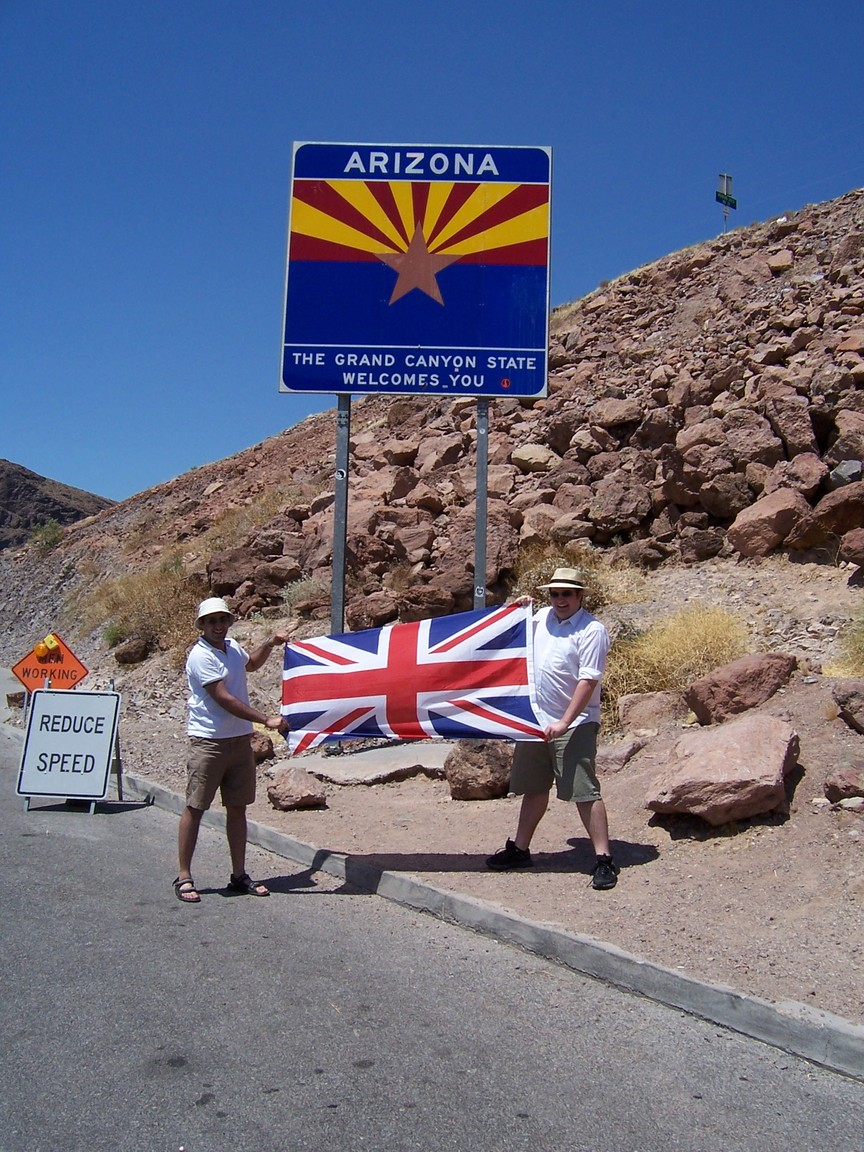
\includegraphics[height=80mm]{gfx/100_1445}\end{center}

After Kingman on Interstate 40 the road straightens out into a long straight highway.  It's certainly sparsely populated but it's not the archetypal Long Straight American Desert Road; this is a quite dull, modern motorway with absolutely no opportunities to pull off at random and make some dust trails.  I am driving and, after a while, I decide the ridiculously conservative speed limit of 75 is just too damn slow.  I disable the cruise control (it is anathema to me in any case) and open the throttle.

Right past a parked, concealed Highway Patrol car.

The car immediately pulls out and begins following me.  After a while he even comes up level with me on the inside lane.

``You should slow down,'' suggests my co-pilot.

``No,'' I said.  ``If I do that, it's like admitting I was doing something bad.  If I just carry on like nothing is wrong everything will be fine,'' I reasoned.

``That's fucking retarded,'' said Imran.

This is obviously a sentiment shared by the police officer.  Despite keeping my eyes fixed straight ahead and not looking anywhere near the car immediately off my left elbow, despite the fact that I know through some crazy E.S.P. that he is pointing a radar gun at my \emph{head}, I carry on as normal.  It doesn't take long for the flashing lights to start and it's only really then that I begin to think I made a mistake.

I panic a little.  In the reams of literature so helpfully provided by our holiday company, none of it discusses how to deal with being pulled over by the cops.  I briefly entertain the idea of opening with a clich\'{e} like ``what seems to be the trouble, officer?'' but decide against it since, well, we all know exactly what the trouble is.  Instead, I sit quietly in the drivers' seat and wind the passenger window down.

``Sir, the reason I've stopped you is, in the state of Arizona, it is not permitted to exceed the speed limit.''

I toy with the idea of asking if there is a state in the Union where it \emph{is} permitted.

The policeman seems a little glum; it's obvious he has looked up our registration and seen it's a hire car.  He asks for my licence and positively crumbles when he hears my (admittedly mid-Atlantic) accent - we are clearly hapless tourists and his usual dose of brutality and degradation may well cause a bit of a political stir.  I feel like a colossal tit as I rummage around to find my licence, naturally it's buried at the very bottom of my suitcase which itself is buried underneath Imrans'.

``What I'm gonna do today, sir, is give you a written warning'' he concedes, holding my Communist State-issued driving licence with obvious disgust.  I feel a small flush of pride as he scribbles `Ponteland, UK' down as my address; the name will now live forever in the vaults of the Arizona State Highway Patrol files.  ``Drive carefully and obey the law, or next time you'll get a fine,'' he warns.  I fantasise about shouting ``DIPLOMATIC IMMUNITY!'' at him but decide not to push it.

In the end I'm given the written warning.  It was for driving at eighty miles-per-hour on a seventy-five miles-per-hour deserted, desert motorway.  Good job, Officer.  We drive off, and I set the cruise control for 75.

It's a wonderful day for driving, perfect weather and clear blue skies.  I'm breaking my hat in and we're eating up the miles, admiring the surroundings.  At Williams we turn north for another hundred miles and eventually our next port of call - the Grand Hotel - comes shooting towards us out of nowhere, all alone on the side of the highway.  It takes me by surprise and I literally burn rubber as I slam on the anchors.  We'd been travelling so long it actually felt strange to be stationary.

Although we have only a limited time here, we decide not to go straight to the Canyon - it's late and we require food.  We discuss the possibility of a helicopter tour but it's just too expensive for me and, besides, the unfortunate fact is we'd have to leave quite early tomorrow and retrace our steps back to Kingman and beyond.  As we dine in the restaurant, the hotel lays on some entertainment for the punters - it's some Native Americans, singing and dancing.  Imran and I feel a little embarrassed - the fate of the Native American people makes me sad at the best of times - and we joke about how they're probably singing about how the White Man killed his culture, land and, well, People - all the while fat white tourists like myself clap with glee at their antics.

There's a pool at the hotel and Imran decides to take a dip - I decide to simply relax on a lounger reading my book (Iain Banks' \emph{Consider Phlebas}) since the pool doesn't look like it's been cleaned since the Colorado first dug its channel into the rock a mile north of us.  Indeed the are floating clouds of copper discolouration which we deeply hope is just bromine.

Afterwards, we sip on some beers and reminisce about old times.  We recall all the childish fun we had as students and also lament how, disregarding our current adventure, Real Life since graduating from University is actually a bit rubbish.

\chapter[Grand Canyon -- Lake Havasu]{Friday, June 3: Grand Canyon -- Lake Havasu}
Immediately after breakfast we head for the `Grand Canyon IMAX Experience'.  I've seen neither an IMAX film or the Grand Canyon and I'm looking forwards to a treat.  We decide that, since we can't really spend enough time around here, watching the film would be the best thing to do since it could cover far more than we could hope to. It certainly was a treat but of course it merely whetted our appetites for more.  We parked up on the South Rim and took a walk to the edge.

For me, the thing which immediately stood out was just how flat the horizon is.  It's almost a mockery of the jagged creeks below; it's almost like you could miss the fact there's an incredible, deadly gorge beneath you.

And then you look down.

Obviously it's beyond my means to describe, simply because my mind cannot make sense of it.  There are giant pinnacles and sheer cliff faces, odd cathedral-like structures that you can just imagine are secret bases for cultist rejects from \emph{Temple of Doom} - some of them even have what look like entrance doors.  And it goes on and \emph{on}.  And it's \emph{really} deep.

\begin{center}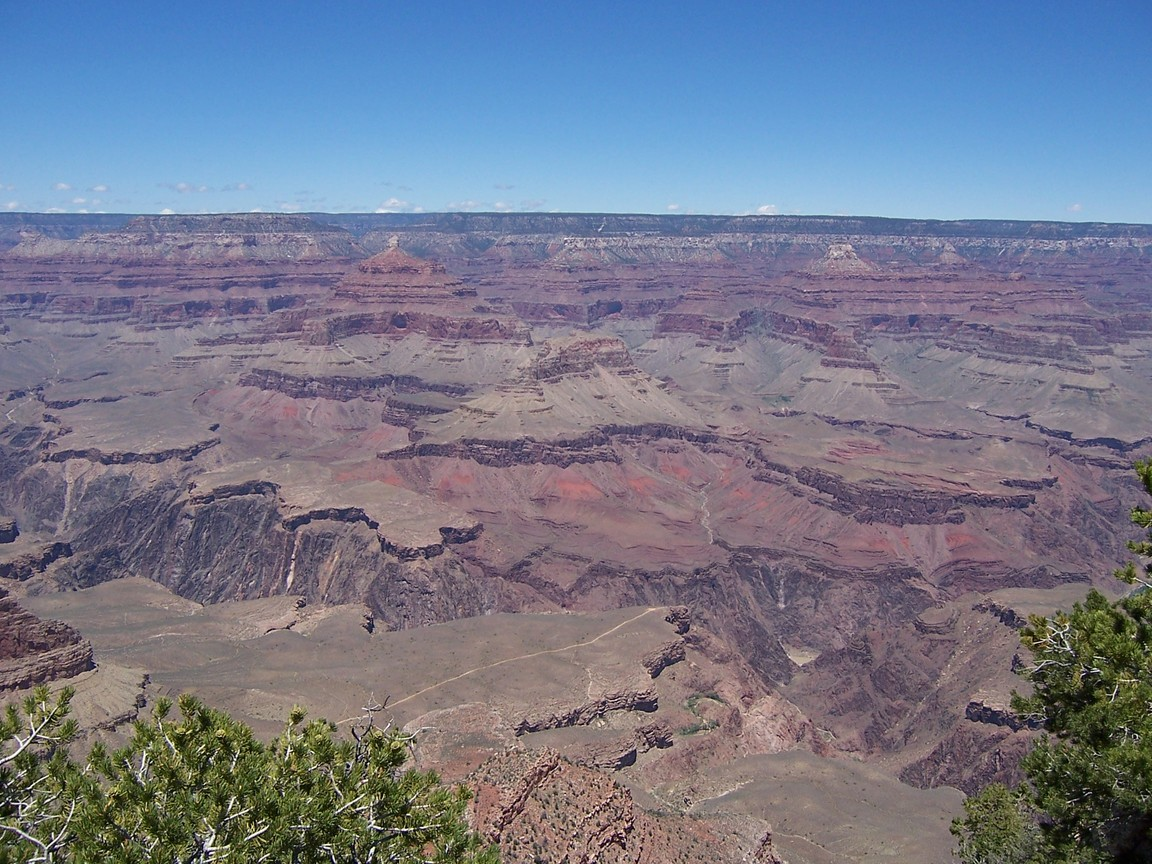
\includegraphics[width=\textwidth]{gfx/100_1458}\end{center}

While chasing a strange-looking insect to capture on film, we strike up a conversation with a travelling band of Ultra-Catholics.  One of them is a girl who is wearing a jumper adorned with Scripture and pink fluffy slippers.  We give her a high-five for style and she \emph{finally} comments on how cool our accents are.  Mission Accomplished.

Time has passed and so we race south, back down the road towards Williams and westwards again towards Kingman.  Thankfully there are no cops and we're free to soak up the sunshine.  As usual, our map would have us follow the Interstate for most of the journey and, as usual, Imran disagreed.  He suggests we `wing it'.  I look at my road map which, rather handily, lists sites of interest and tourist spots and I'm finally convinced to agree by two things -- first, a site marked `ghost town' and second, a site marked `Black Mesa'.

Now, as any good \emph{Half-Life} fanboy knows, the Black Mesa Research Facility which features as the setting for the first game is actually in New Mexico - but I wasn't about to let that fact ruin the thrill of visiting a completely different fictional location and so I acquiesce.  We turn off I-40 just after Kingman and onto a single-carriageway barely paved road leading, seemingly to nowhere.

I decide I love Arizona right there and then.

\section*{Kingman and Oatman}

Before long we get as close as we can to `Black Mesa' and park up; it's apparently still miles away and we can't really see anything black or mesa-like.  What we \emph{can} see, though, is a large butte sticking out of some scrubland a way off the road.  We both need to answer nature's call and so decide to wander up to this huge clump of rocks and, well, wee on it.

\begin{center}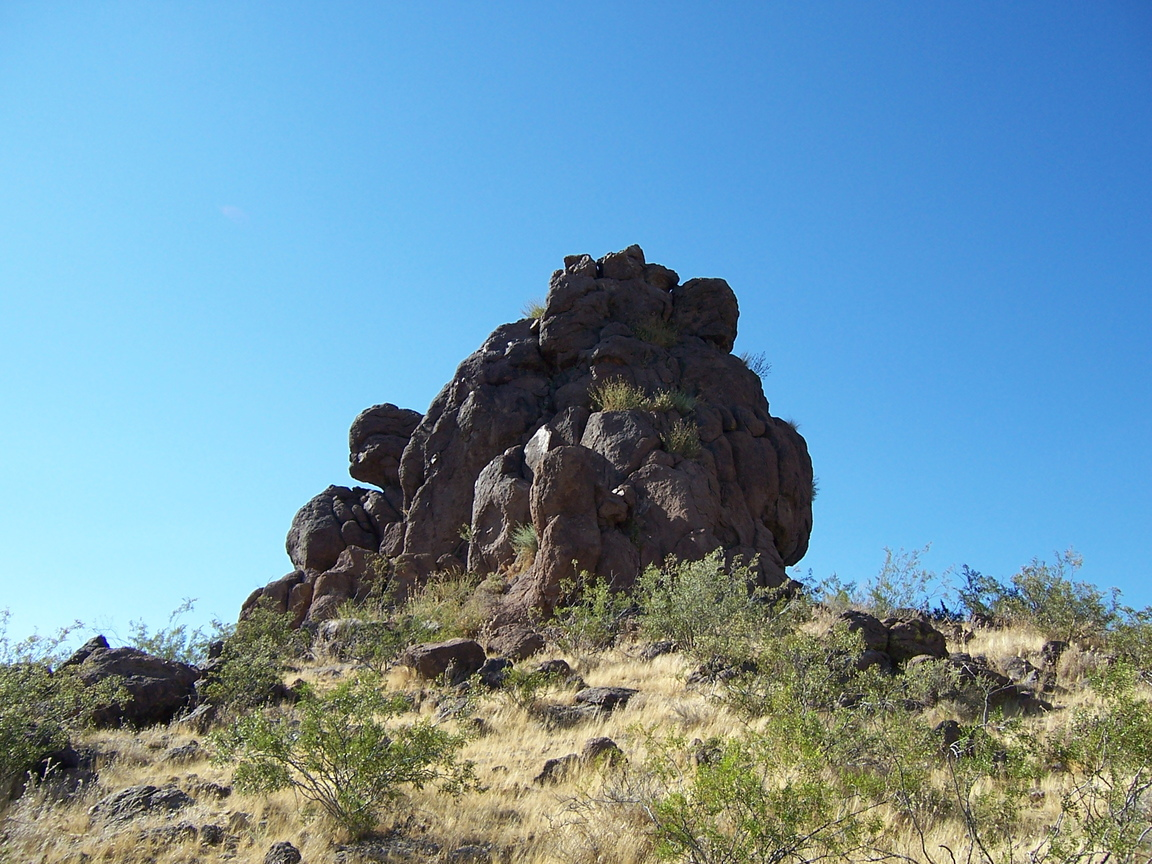
\includegraphics[width=\textwidth]{gfx/100_1521}\end{center}

En route we dodge strange cacti - we're fascinated, having never seen one up close before.  We are surrounded by desolation punctuated by electricity pylons and, on the horizon, we can see hills (and indeed, something that looks like a dark mesa...) and nothing else.  As we climb the butte, we worry about snakes - but mostly we worry about being eaten by the Graboids from \emph{Tremors}.

\begin{center}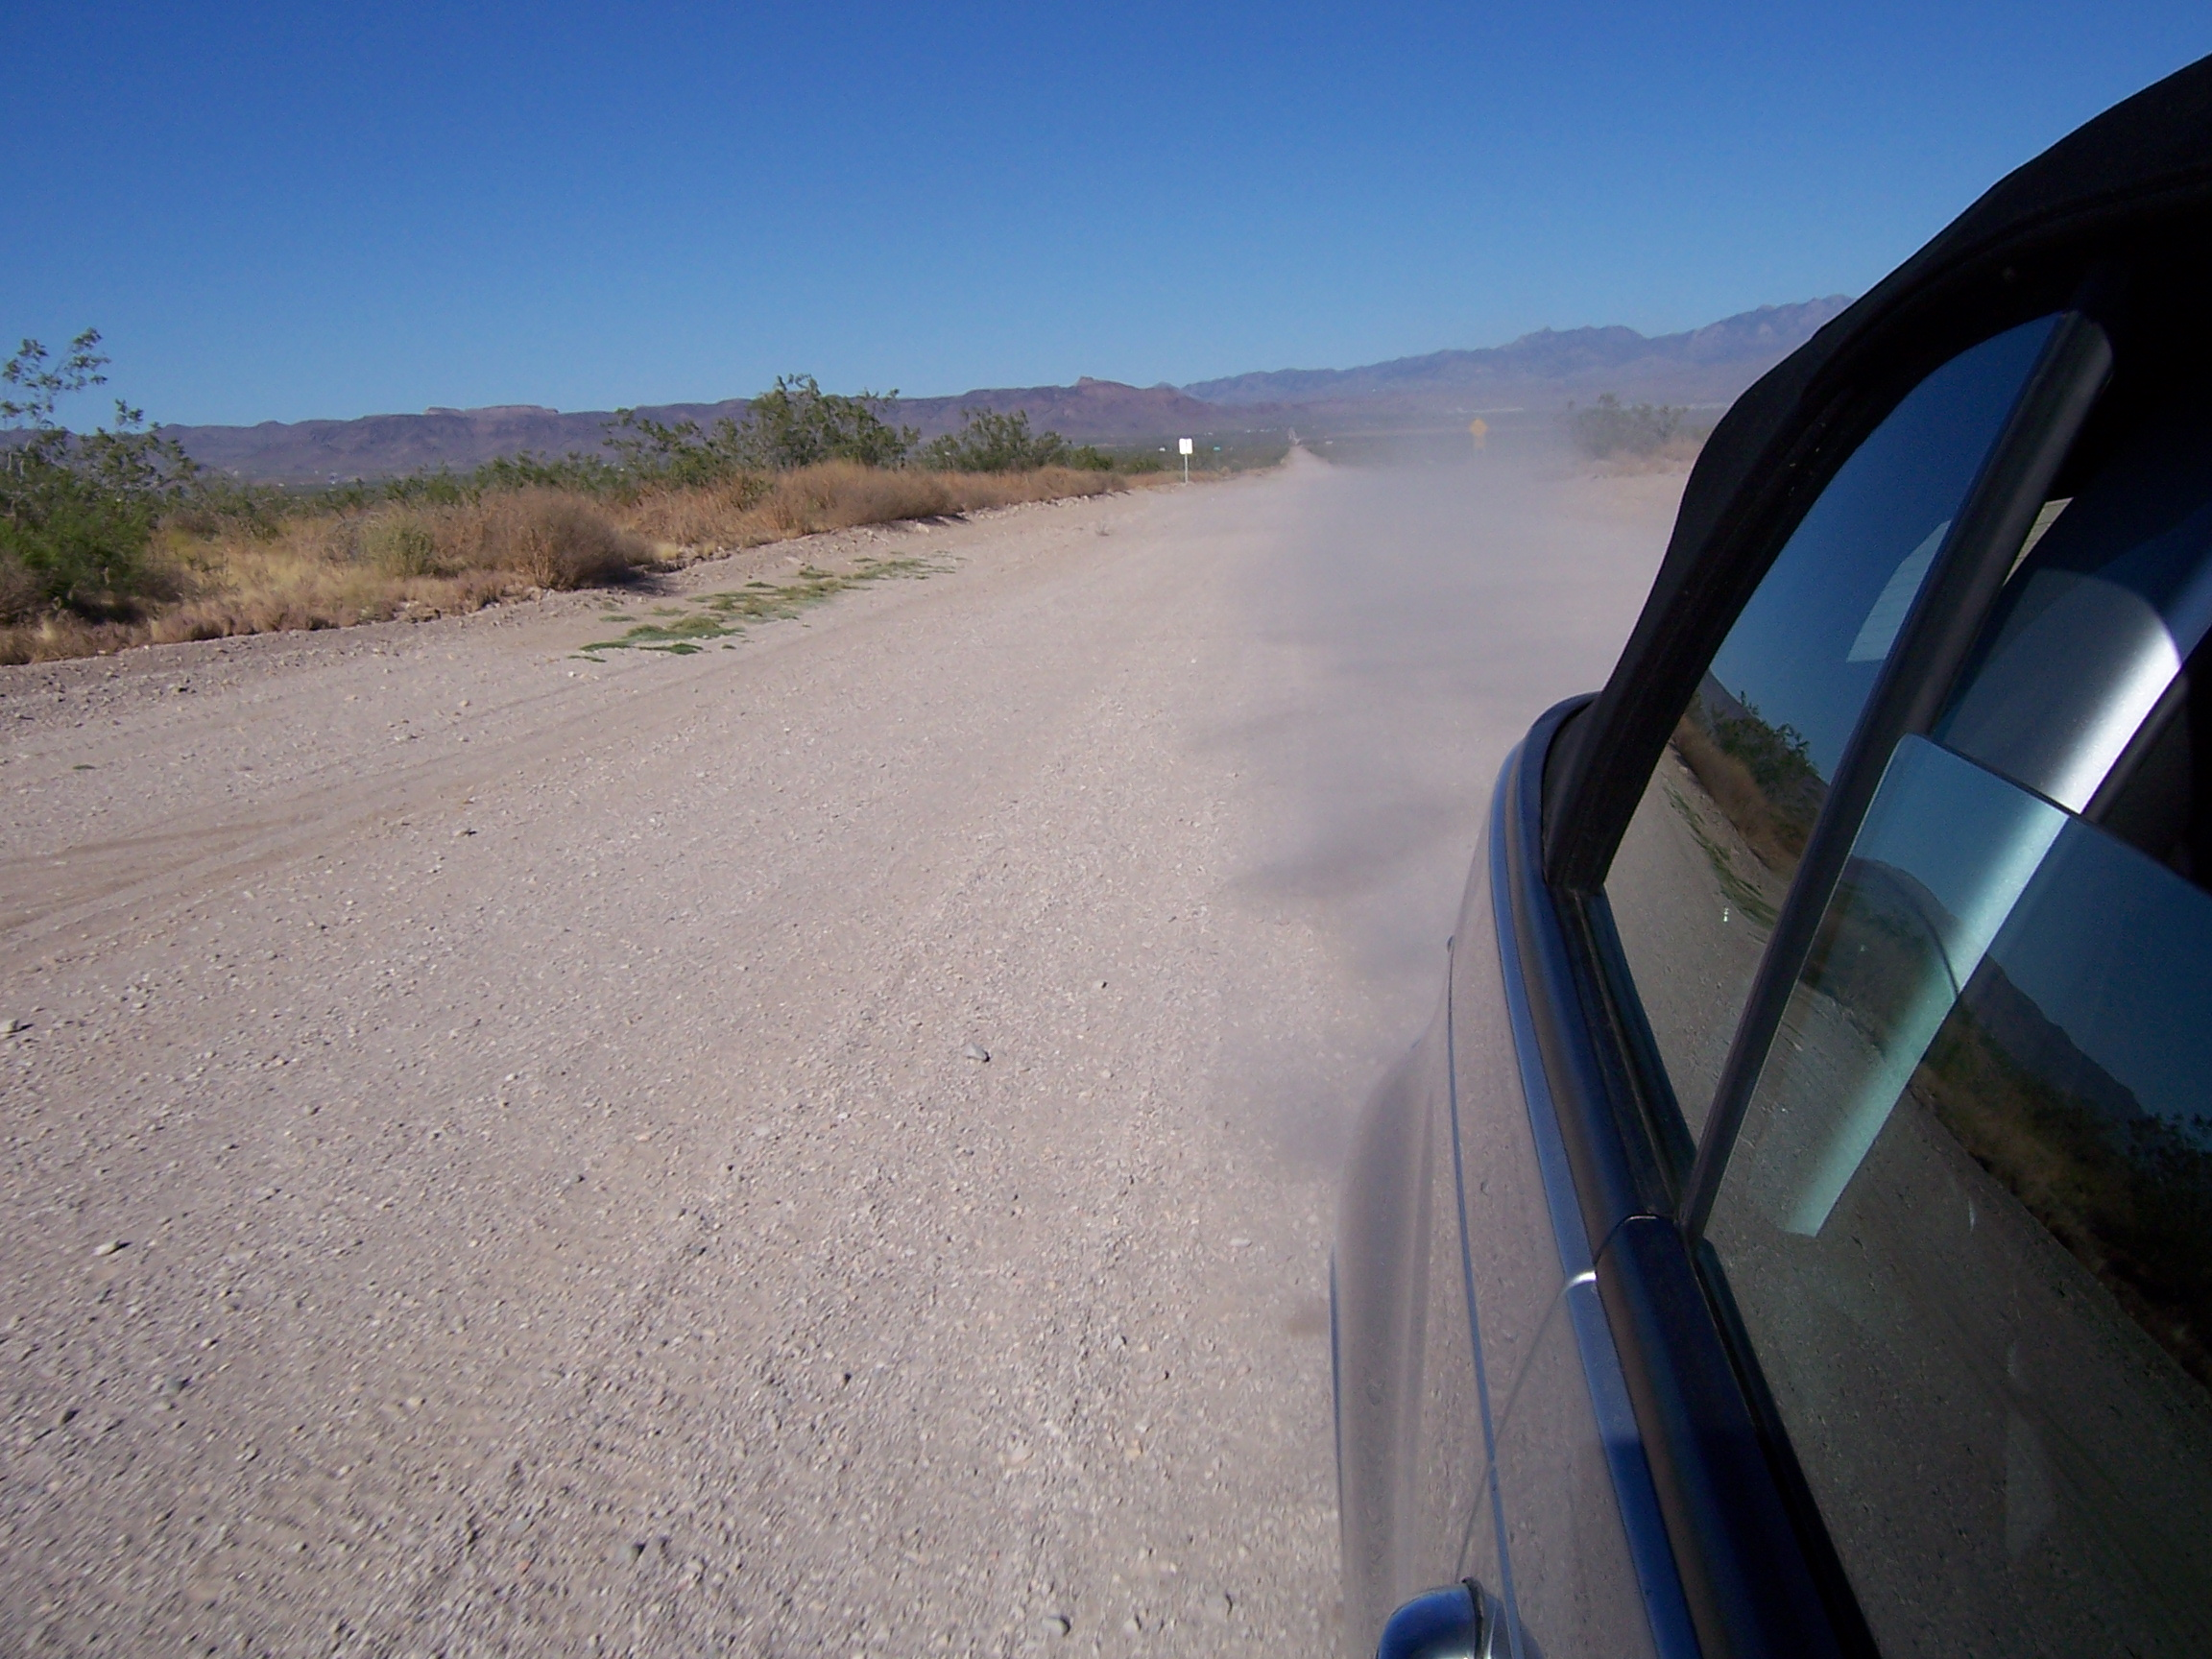
\includegraphics[width=\textwidth]{gfx/100_1531}\end{center}

Eventually we depart and head down what according to my map is an alternate route to Lake Havasu, following the road due west.  Before too long it turns into dust.  At regular intervals we cross roads laid perpendicular to us which are nothing more than ditches - sometimes not even that.  They lead nowhere that we can see; our road seems to be taking us straight into a hill - we have faith that there will be a pass up and over the hill at the end.  The roads crossing us have, at first, fairly romantic names - Tombstone Trail, Desert View Trail, Teddy Roosevelt Road.  When they run out we cross Agate Road, Flint Road, Garnet, Zircon and Jade Roads.  Finally we cross roads named for Native American tribes - Havasupai, Hopi and so forth - presumably named after the people who were here before being replaced by a series of isolated caravans.

People obviously live in these trailers (indeed I later learn this is a township called `Golden Valley', which sounds both romantic and like a filthy Karma Sutra manoeuvre) and we get the ominous feeling that we really don't belong here.

We put pedal to metal and hurtle west, the hill ahead of us looming ominously.  Massive plumes of dust billow out behind us - in the clear air and flat surroundings they can be seen for miles.  Any minute now the trail will turn left - south - and lead us home.  Some people are coming out of their trailers to watch us.  We worry about hillbillies and again, more than ever, Graboids.  Of course, any film connoisseur will inform you that \emph{Tremors'} Perfection is in Nevada but, again, shut up.

\begin{center}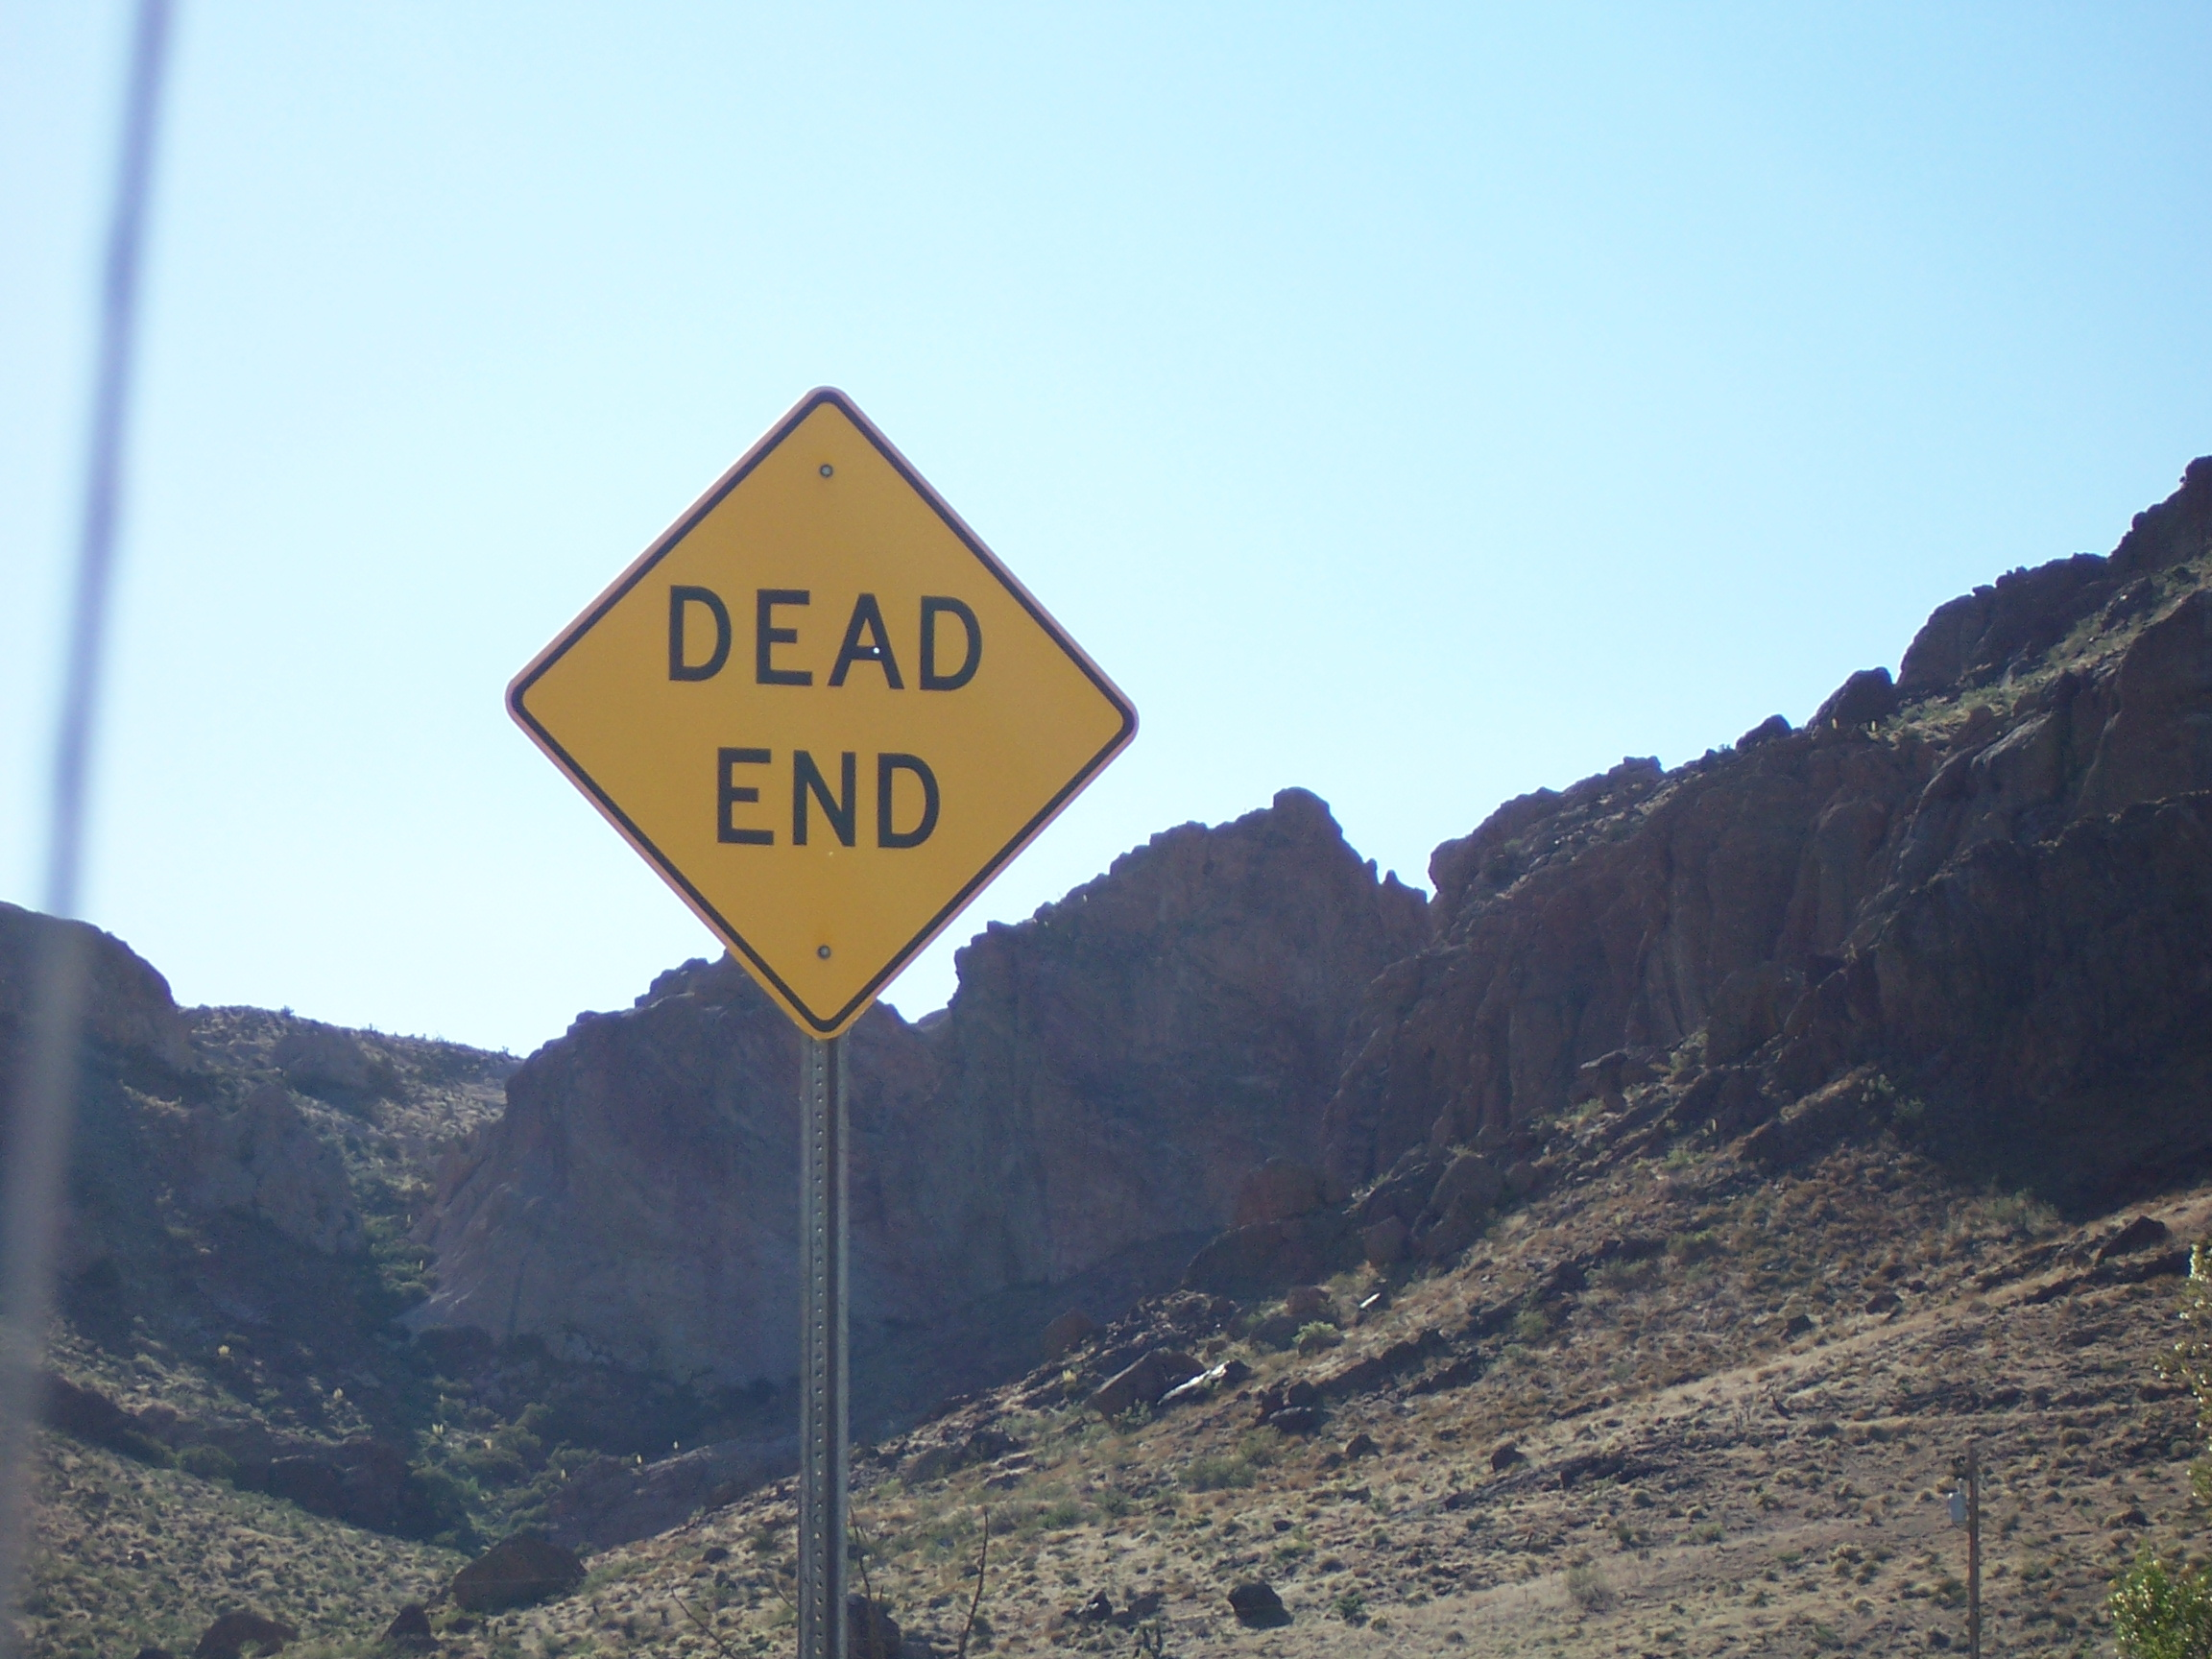
\includegraphics[width=\textwidth]{gfx/100_1536}\end{center}

Then we run out of road.

No southbound turn.

No route over the hills.

Just a sign, ridiculously and superfluously pointing out the `dead end'.

There's nothing for us to do now but drive back through our own dust clouds back to the interstate, which we begin to do.  We pass a dilapidated caravan in a fenced-off lot; along the side of it is scrawled in red paint `for sale' and a telephone number.  We fantasise a little about buying it (it certainly looks cheap enough), doing it up and using it as a holiday cottage.

I'm actually starting to warm to Golden Valley - there are magnificent views of the Black Mountains to the west, Hualapai Mountains to the east and glorious, flat, empty desert plains north and south.  Some day I may choose to live there, but right now, the clock is ticking and we're miles from home.

We reach the butte again and realise that there is another road running almost parallel to the one we've just had the abortive experience with, and it looks just large enough to be the one on my map.  We follow it and, sure enough, we cut through the desert and, finally, begin to rise up over the mountain ahead.

Nestled high up we run into a gas station - just as well since, once again, my blood pressure is heightened by our dwindling fuel supplies.  Unfortunately for us, it looks like it has been abandoned since 1950.  It makes up for it, though, by being in that classic 1930's style that brings Route 66 to mind - it's the first time we've seen anything like it.  Second, just left of it is a huge saguaro cactus, standing proud and defiant.  There is nothing more `Arizonan' in my mind, and I fall in love a little more.  Driving on, we're surprised to see that despite our blunders and for all our `winging it' attitude, we are actually travelling on Historic Route Route 66 itself - there are respectful, reverent signs informing us so.  It feels like fate.

\begin{center}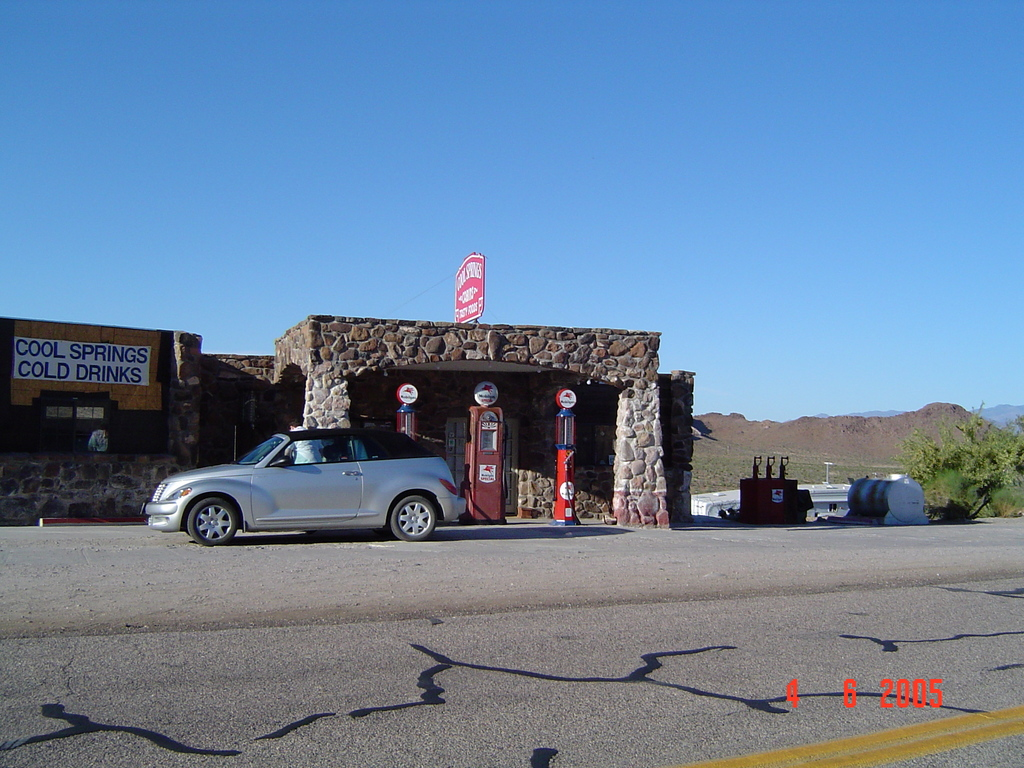
\includegraphics[width=\textwidth]{gfx/DSC00700}\end{center}

As we crest the hill, we see a beautiful expanse of terrain beneath us, sliding away to the horizon.  Dusty green plains stretch dramatically out and away, ruffled and undulating like a thick quilt, punctuated by small hills and yet more buttes.  It's truly breathtaking.  The road is incredibly winding and we drive like we're a rally team, zigzagging down to meet the soft, springy carpet of the land beneath us - we both spontaneously cheer and whoop with the sheer pleasure of it all.

After a while we pass through Oatman, once a dying mining town that has since reinvented itself as a tourist spot - there are saloons, wild roaming donkeys in the streets and old-timey restaurants featuring places to tie up your horse.  It is the very last thing we expect to see out in this desolation and driving through it feels incredibly surreal.  Crucially, though, there is no gas station and so once again I petition Imran to continue our descent in neutral.  He laughs me off.

The sun begins to sink toward the horizon and the air begins to chill as we plough south through the glorious countryside.  At this stage our map is of no help at all; we have no idea where we are and no idea how far our destination is until, finally, salvation - we hit a main route complete with helpful signposts and, thank goodness, a gas station.  We fill her up and, pointed without a doubt in the correct direction, zoom towards Lake Havasu City while watching the sun set behind the hills on the western horizon.

\begin{center}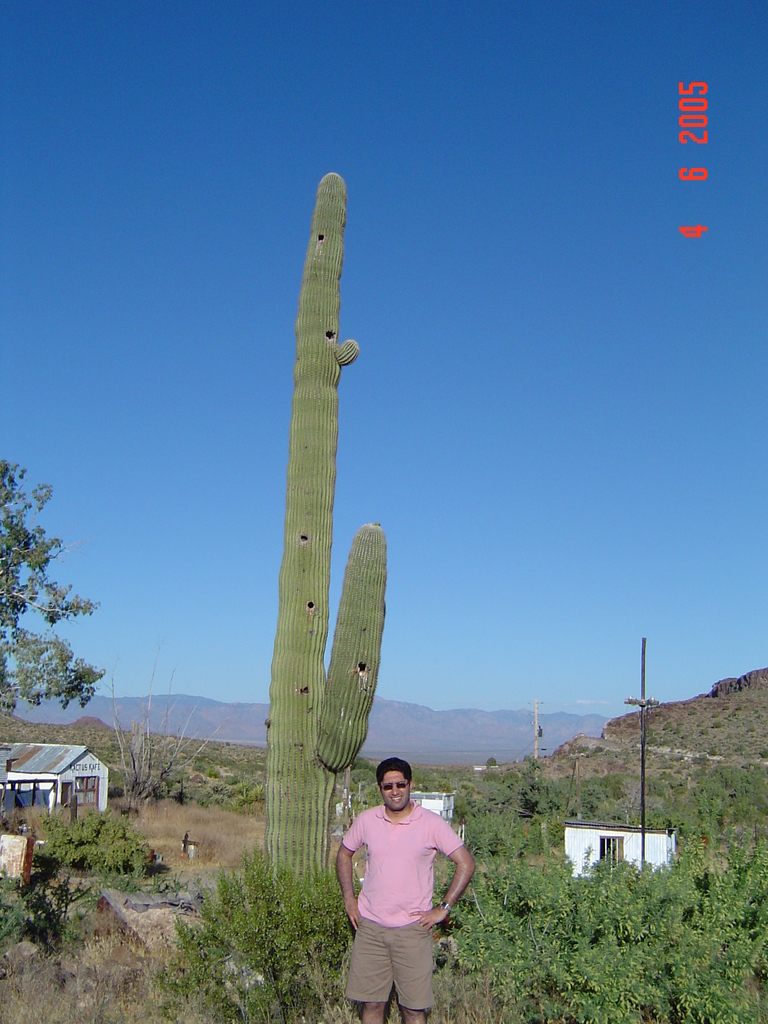
\includegraphics[height=100mm]{gfx/DSC00701}\end{center}

On the way we pass a varied array of huge pick-up trucks, shiny 4x4s, all manner of powerful vehicles and all of them towing trailers on which are secured a cornucopia of beautiful powerboats and pleasure yachts.


\section*{Lake Havasu City}
When we finally reach civilisation, it's very dark and very late.  Our maps and route plans do not tell us how to get to our hotel so we're navigating using the Force; it's only really been sheer fluke we've done so `well' so far.  Tonight, though, our luck runs out and we cruise up and down through the mean streets for a good long while.  Our only clue is the hotel's name - \emph{Nautical Inn} - so we assume it is somewhere close to the lake itself.

As it happens it couldn't \emph{be} closer to the lake - it's on a bonkers island, not far out off the shore but enough to throw us off the scent.  Eventually we arrive and unpack the car to the noise of wild partying - there are cool hip young people wandering about and we see a lively bar built on pontoons bobbing about on the water, just off the hotel's private beach.  All thoughts of travel-weariness disappear in a flash and we silently agree that this is the place we need to be at.  I throw my trusty Union flag over the balcony of our room to let everyone know there are cool, well-travelled eligible bachelors in the hizzouse (no-one actually cares).  We freshen up and throw on our best clothes.  Imran loans me some of his ridiculously expensive - but \emph{oh so worth it} hair sculpting wax and I reverently shape my coiffure before we head on out.

We enter the \emph{Naked Turtle} Bar and immediately smell \emph{money}.  It's clear the people around us are minted and, to a person, \emph{beautiful}.  Men, women, young and old - they all sport firm, muscular bodies and perfect teeth.  We do our best to fit in and start to gulp down cocktails.

Before long we strike up a conversation with a couple of people at the bar and exchange gossip - there's a kid there from Orange County (of which my only knowledge is `posh suburb of Los Angeles' and `they made a TV drama about it') whose dad has just bought a new place in Lake Havasu City; he is in town to try out his new boat.  We douse the flames of envy with our booze and decide not to employ our usual fa\c{c}ade of being plastic surgeons given that we are, in all likelihood, surrounded by either:
\begin{enumerate}
\item plastic surgeons,
\item spawn of plastic surgeons,
\item clients of plastic surgeons or
\item all of the above.
\end{enumerate}

We're introduced to a guy about our age called Bob.  Bob looks cool; he has a Lynyrd Skynyrd t-shirt, a labret piercing, an imperial beard and a shaven head.  He insists we order some tequila with him and come on over to party with his buddies.  We readily agree but we don't know the first thing about tequila.  ``Don't worry,'', he says.  ``Just get the best - Jos\'{e} Cuervo.  This shit \emph{fucks you up!}'' \\
We order Jos\'{e} Cuervo and follow Bob.

He takes us to a group of cool-looking cats - three guys, three girls - and introduces us, before proceeding to get horrifically drunk.  Later on our new buddies will admit they have no real clue who Bob is; he is `just some random dude'.

We get on very well; there is a mellow dude in a backwards hat and many piercings who I'll call Ozzie; his rambunctious lady who I'll call Harriet; a guy in a smart shirt who is built like an American football player called Ryan; a dark, spiky haired fellow called Dan and his dark, elegant lady Lisa; and Britta, a high-spirited Sarah Chalke lookalike.  We gossip and relate our tales of the Road, they listen attentively and talk about their lives.  Bob steals my camera and takes pictures of himself flipping The Bird.

I'm filled with Dutch courage at this point and notice that Britta doesn't have a man to guard her.  I move in for the kill.  We have a round of drinks together; we laugh and take pictures of each other --- well, I imagine she would had she a camera, mostly it was just me taking the pictures --- and she offers to show me her ludicrously expensive ring.  As it happens, it's her birthday and she has just been given a Tiffany ring as a gift by someone quite close.

It's then that I realise I've spent the last hour chatting up Ryan's girlfriend, \emph{right in front of his face}.

Not really knowing who or what Tiffany's is, I pass comment that it really doesn't look all that expensive.  Ryan's face visibly sags.  Britta does not talk to me again.

Soon after we're joined by Dwaine, who is tanned and sports very manly stubble.  He tells us that they are all spending tomorrow on Dan's powerboat and suggests we join them on the lake.  Dan agrees; we nod vigorously and give him our room number.  He tells us to expect a call in the morning and we, fall-over drunk, retire.

\begin{center}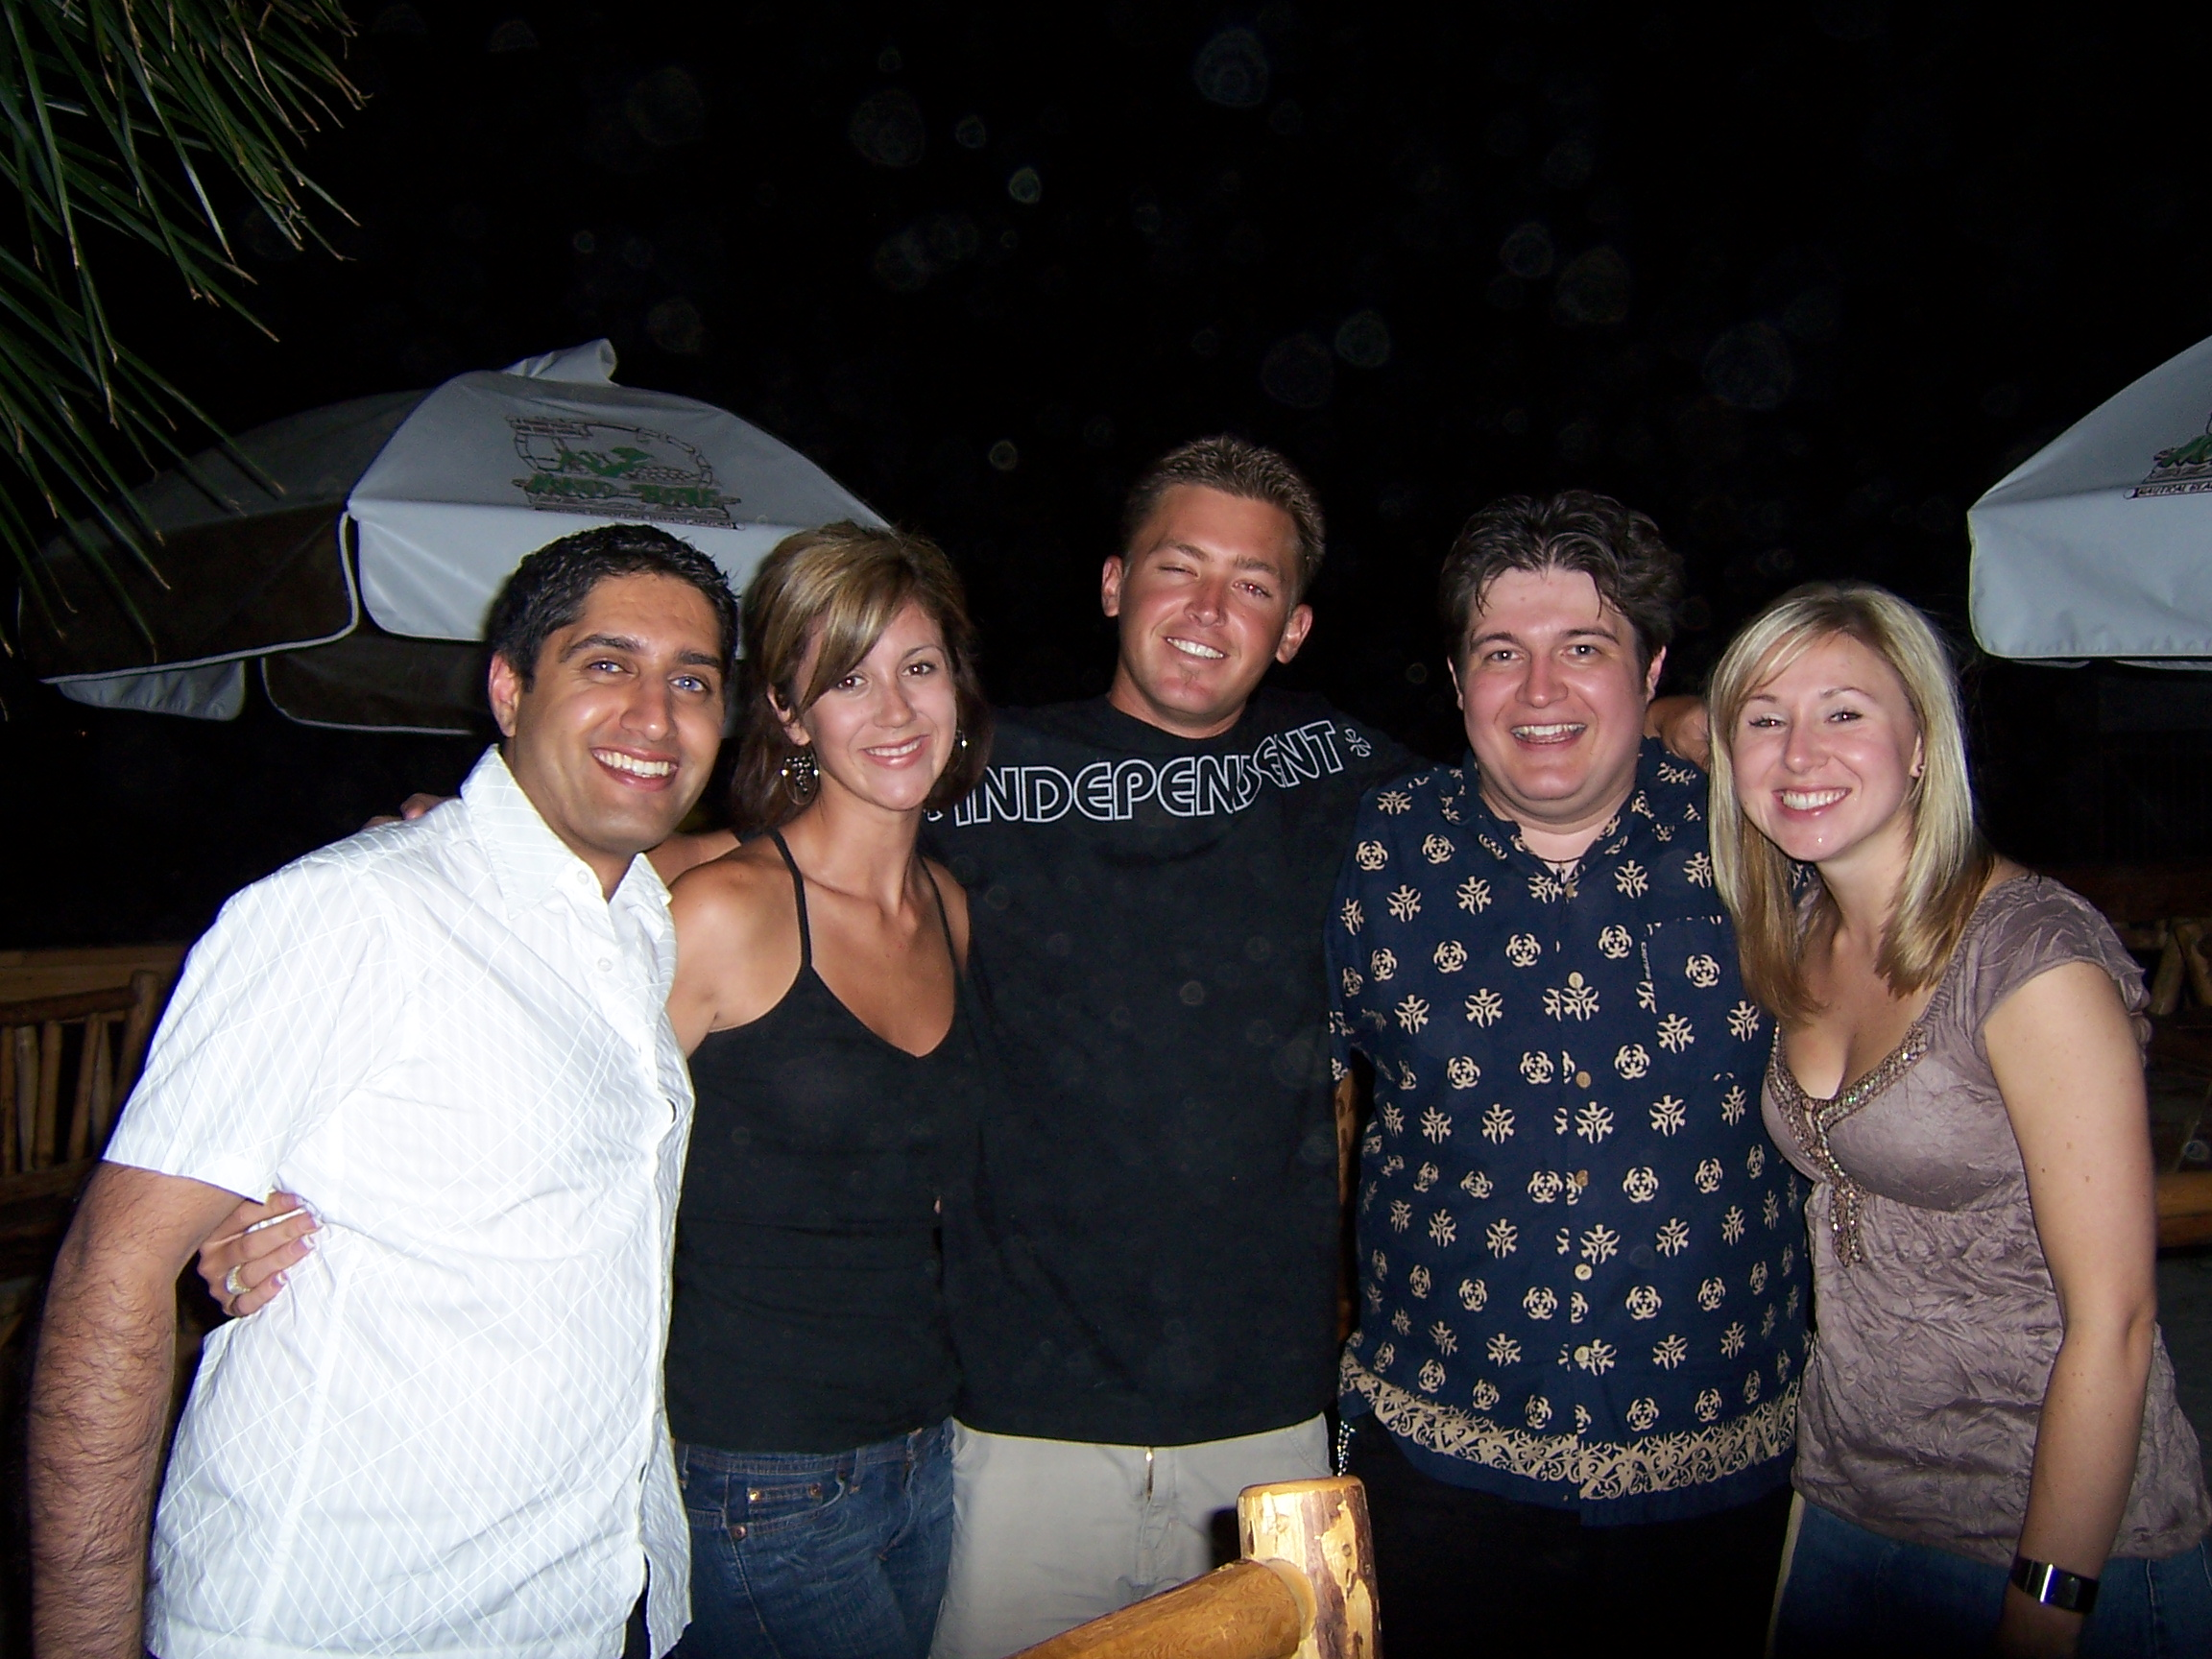
\includegraphics[width=\textwidth]{gfx/100_1579}\end{center}

\chapter[Lake Havasu -- Palm Springs]{Saturday, June 4:  Lake Havasu -- Palm Springs}
We awake horribly hungover and deliberately sleep over the time we had agreed to be up and ready by.  Both myself and Imran secretly and independently decide that getting out of bed and boating with strangers is a rubbish idea and that we should just sleep until midday instead.

Then the phone rings.

Of course it is our new buddies; they are getting ready to hit the water and would pick us up at the marina in a little while.  With infinite reluctance, we heave ourselves out of our beds, cleanse ourselves and pack our bags to stow in the car before heading to the hotel restaurant.

Over breakfast, a bizarre occurrence:  the lady in charge stops her patrons mid-muesli and loudly announces that her spiky-haired waiter, a stocky teenager, would like to sing us a song.  The boy, looking every bit the television pop talent contest runner-up, grins sheepishly and immediately serenades the breakfasters with a disgustingly saccharine, typically \emph{American} R\&B ballad \emph{a capella}.

We clap politely and return to our toast.

It's a beautiful day; the sky is cloudless and the shimmering waters of the lake look enticing.  Boating is not something I had in mind when I packed my suitcase and so I decide to pay through the nose for some flip-flops at the conveniently located nautical equipment store attached to the restaurant.  After that we proceed to the edge of the conveniently located jetty which is conveniently attached to the nautical equipment store.  Our friends sweep towards us in their boat and we embark.

\begin{center}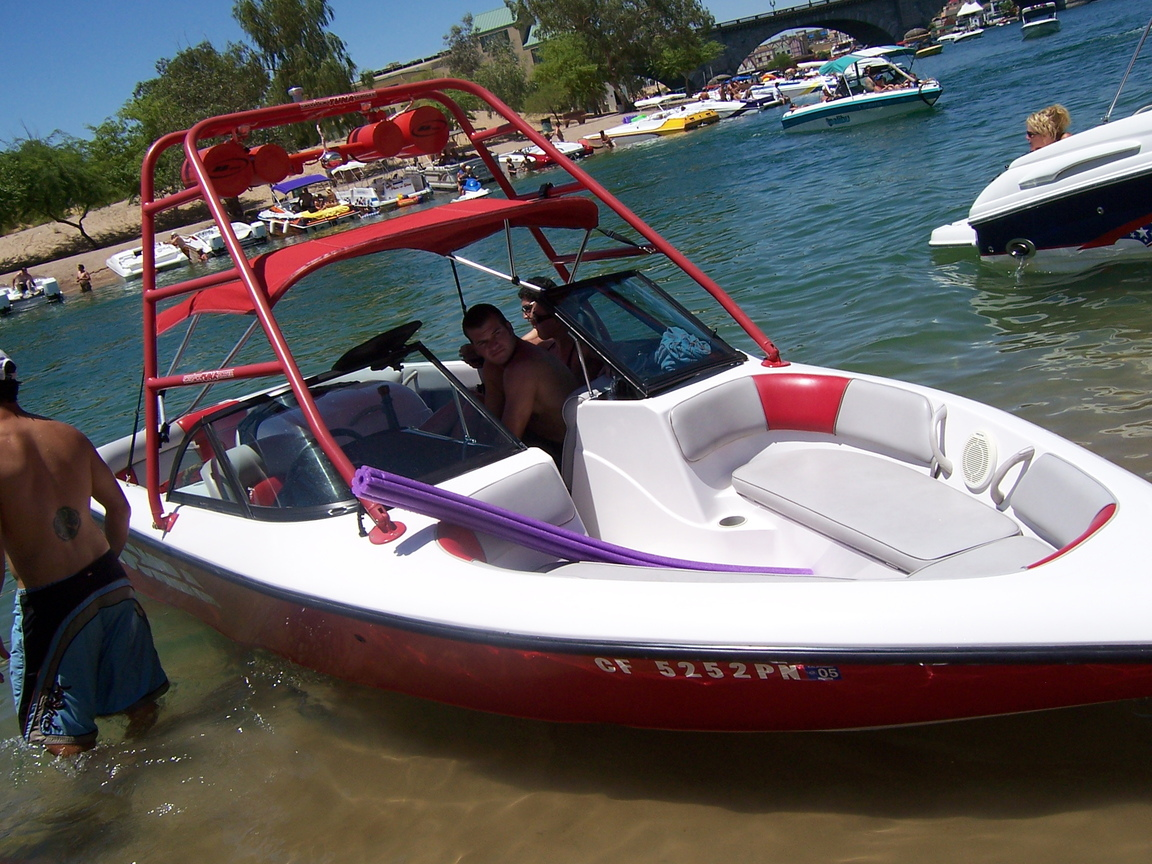
\includegraphics[width=\textwidth]{gfx/100_1606}\end{center}

And what a boat it is; it is large, powerful and majestic.  It is even a little pimped-out; the various metal tubes forming the canopy over the cockpit are dripping with speakers.  Clearly out here they take such things very seriously because we see a number of boats which appear to be nothing more than floating subwoofers all piloted by chiseled and tanned looking rich kids.  It feels like we've wandered into \emph{Dawson's Creek}.

There are comfortable, spongy seats curving around the inside of the bow; enough room for four.  Behind that is the pilot's seat on the starboard side and, portside, more seating for three, all covered by a canopy.  In the stern are seats for three more.  Most of the seats are filled with people and what space is left is filled with cans of beer.  Ryan and Britta sit forwards and blank me for the entire day (fair enough, I concede).  Amidships are Imran, myself and Dan, who is piloting.  We're not sure if it's his boat or his fathers and we suck up to him immensely.  In the back seats are Dwaine, Jackie, Lisa and a small dog wearing a life jacket.  There is also, as previously mentioned, a great deal of beer.

We honestly weren't expecting it, but it seems the plan for the day is to simply drink beer, listen to music, chat and sunbathe - but \emph{on a boat}.  Periodically we speed up or down the lake just for fun.  The spray flies into the air and soaks us.  We drink their beer and really begin to feel like we're taking the piss just a little, but raise a glass to American hospitality nonetheless.  Just to save face, we promise that we would have brought a crate of beer of our own along had we known in advance.

%\begin{center}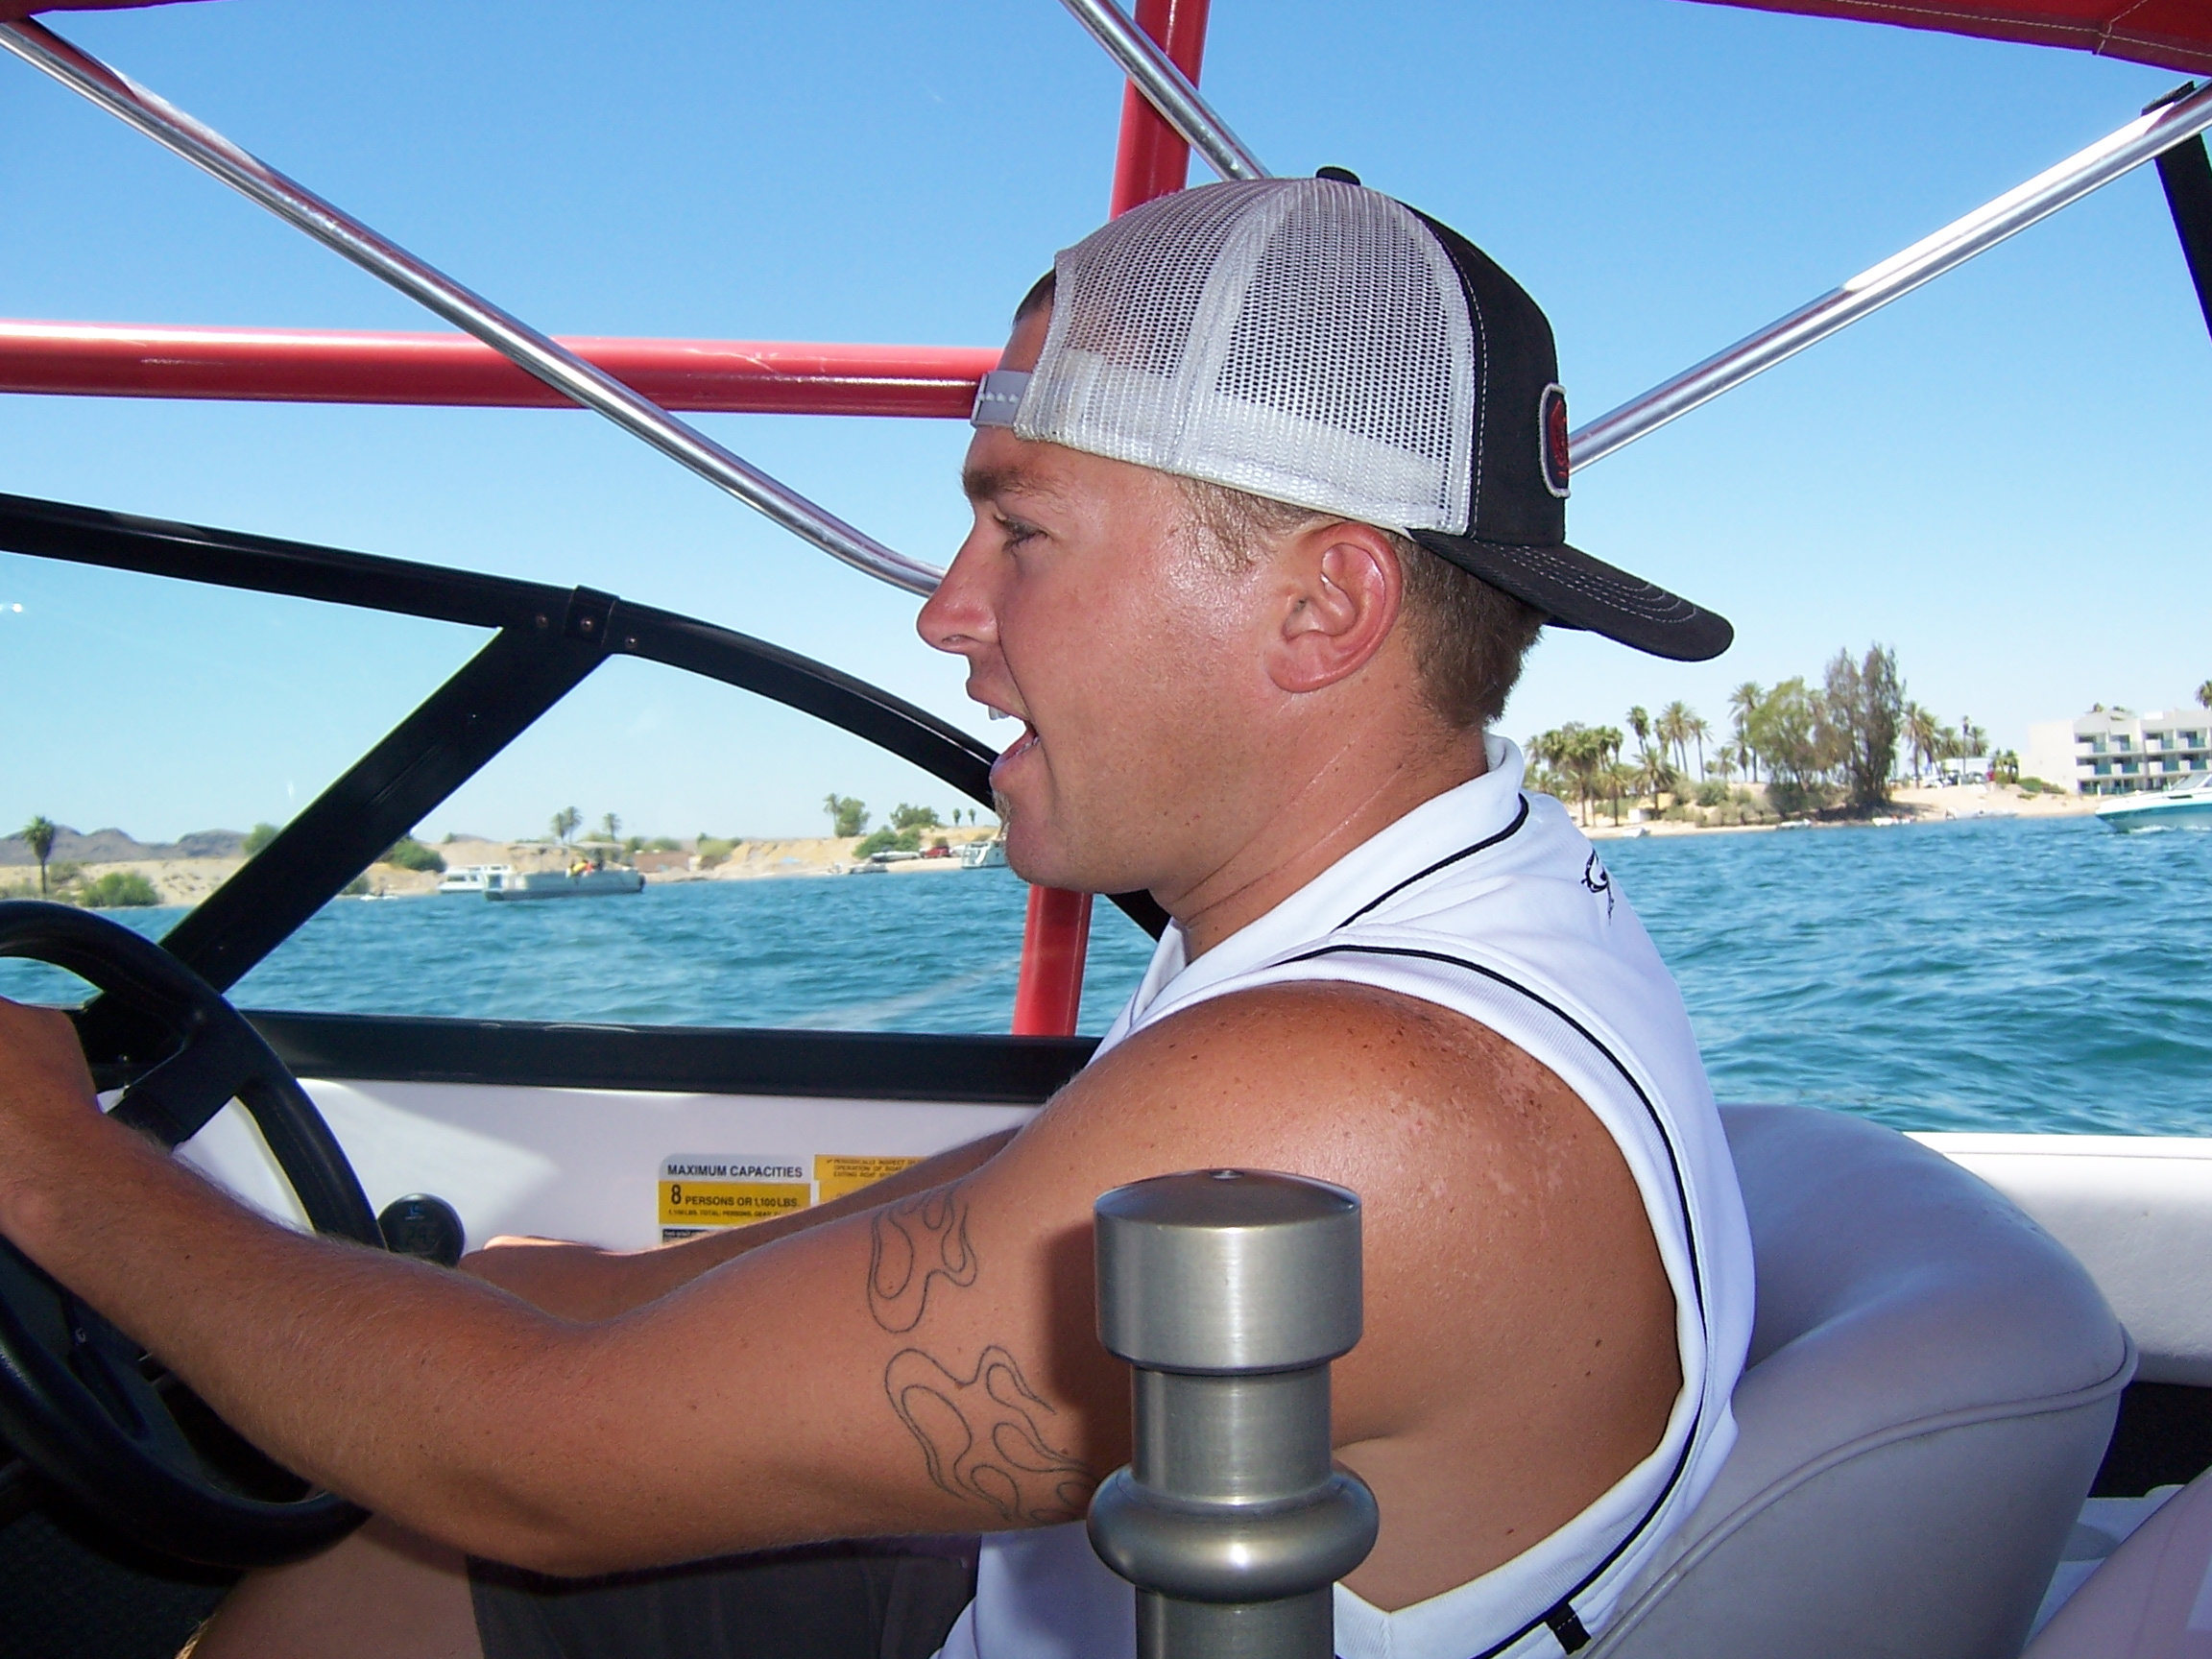
\includegraphics[width=\textwidth]{gfx/100_1587}\end{center}

We chat and pass the time; Lisa talks nonchalantly about her planned breast enlargement surgery.  We assure her she does not need it.  The sun beats down and the men strip off their t-shirts.

I keep mine on.

The lake is buzzing with boatfuls of people doing the exact same thing we are; music blares from north and south and boats decked out like floating shops whose sole mission is to sell snacks and drinks tack up and down like the tuck shop of a world-class youth club.  Dan pilots us to `London Bridge'.

A quick word about London Bridge, then.  We learn that Lake Havasu City is apparently famous for owning the \emph{actual} London Bridge.  But how can this be so, you ask?  Surely London Bridge is still in London?  You've probably fallen into the same trap I did - that of confusing it with Tower Bridge, an altogether more memorable structure.  \emph{This} London Bridge did indeed once cross the Thames but was sold to an American chainsaw magnate because it was falling down, falling down.  He founded Lake Havasu City, shipped the chunks of the bridge through the Panama Canal and rebuilt it here (while, of course, a new bridge was built in London).  Actually he only used the original chunks as cladding - the core of the bridge was brand new - something I feel is a bit of a cheat.

Frankly I found it unimpressive; not even the rows of little Union flags flying along its length nor the Olde English-themed shopping mall at the eastern end could save it - in the end, it is just a bridge.

\begin{center}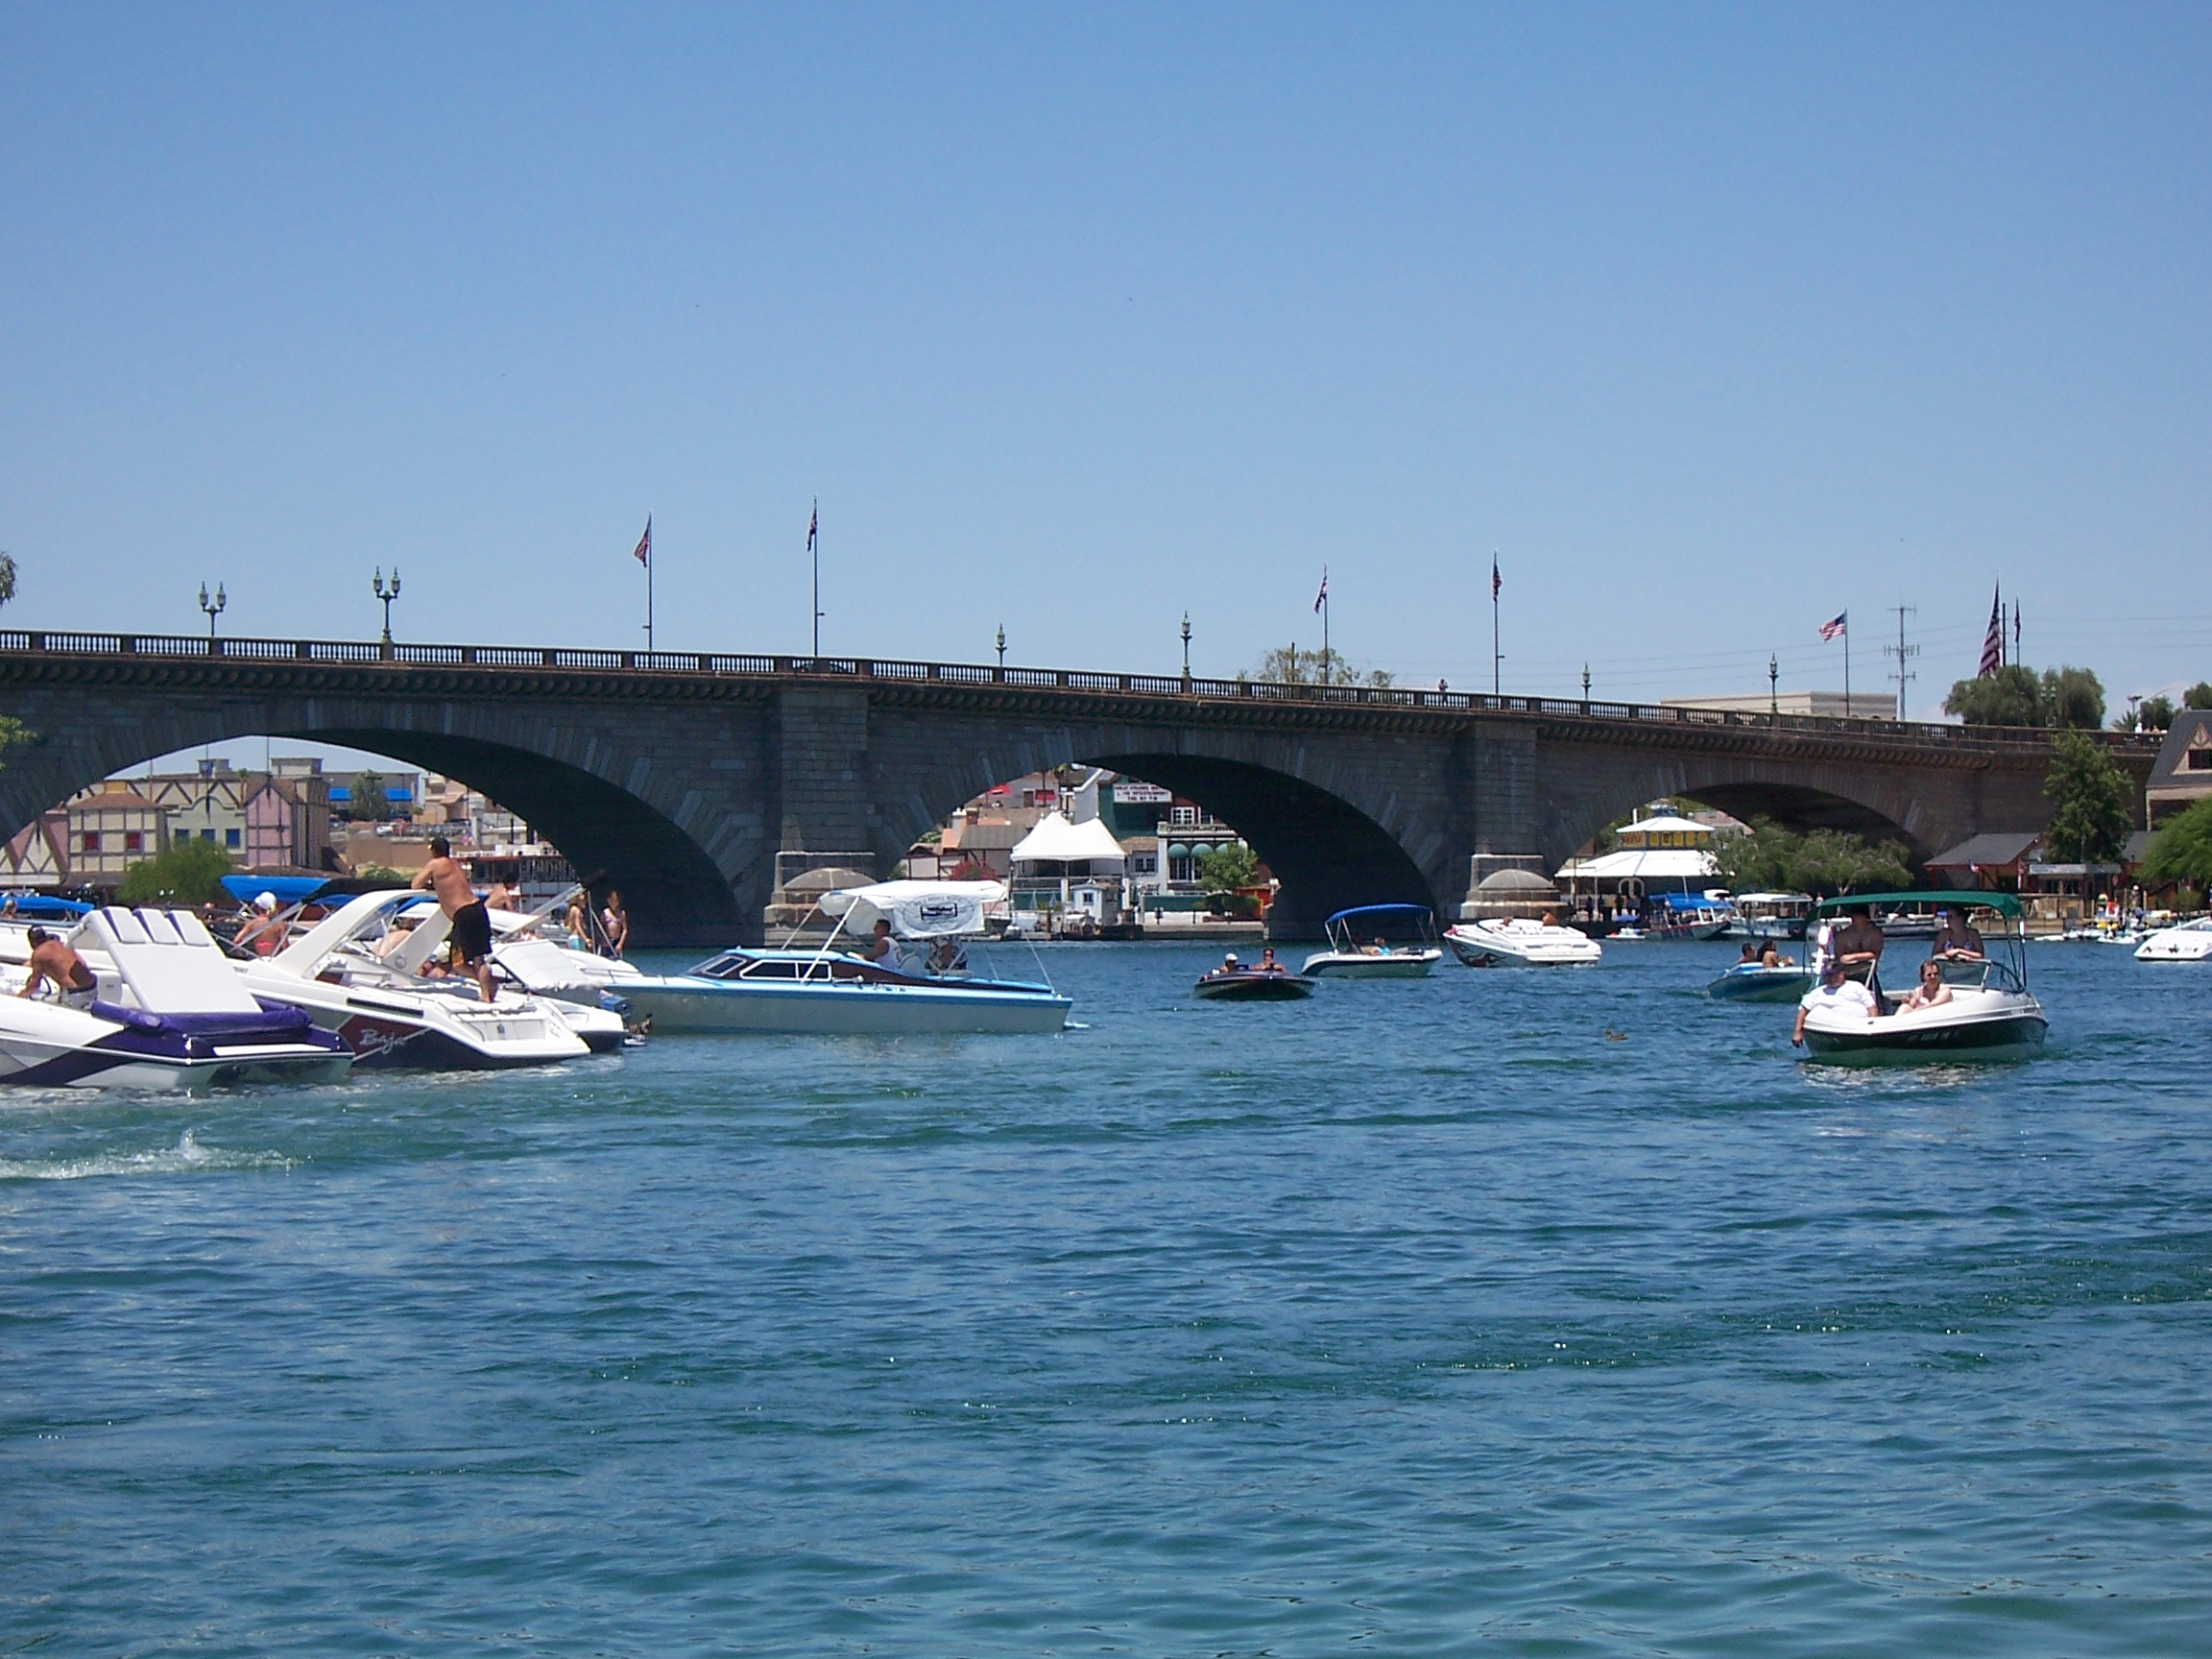
\includegraphics[width=\textwidth]{gfx/100_1598}\end{center}

The boat turns around and heads south.  Lake Havasu is little more than a serpentine bulge in the Colorado River on its way to the Gulf and we head down it a little way before anchoring in a cove on the western shore.  There are tens of other boats here, all filled with revellers.  There are cool young people swimming, sunbathing, talking and drinking.  It is also very loud, very much like a nightclub.  There is a comical moment where all the music suddenly stops and all drinks are hidden as a police boat enters the cove.  The episode brings to mind a naughty child being checked up on by its mother; I also smirk at the idea that these people could be wealthy and adult enough to be entrusted with a large, expensive, powerful motorboat but still have to hide their can of light beer at the sight of an authority figure.

Our buddies and Imran dive into the warm water and swim around the boat, laughing and splashing.  Surrounded by such perfectly sculpted meat, I begin to feel incredibly self-conscious and simply sit in the boat, fully-clad, baking in the sun.  I begin to wonder if there is some way I can bolster my shattered self-esteem and regain some of my cool - and then I see it.

Jutting out into the water is a high promontory.  It is easily climbable from the shore but terminates in a fifty foot plunge into the cove.  At regular intervals we see whooping daredevils climb up and hurl themselves off, much to everyone's delight.  I cast my mind back to the summer before, camping in the Lake District, where I had leaped off a broadly similar rock into a broadly similar body of water (although naturally the water was a lot closer to absolute zero).  I stare at the perilous drop and begin to believe that \emph{I can do that}.

I announce the fact that I am going to throw myself to my doom and immediately my street cred is elevated.  I jump into the water, still in my Penny Arcade `It's not my fault you suck' t-shirt, and swim to shore before beginning my climb up to the sky-piercing peak.  A tweenage boy follows me.  After a little while I reach the top and look down into the cove.

It's a \emph{really} long way down.

I chicken out.

No amount of looking manly is worth a fifteen metre freefall.

I turn around to climb back down and find the narrow way blocked by the young boy.  He won't let me past. ``Come on, dude, you can do it'' he urges.

``I can't do it,'' I whinge.  ``I wanna get down.''

He doesn't budge, and by now, it's too late - everyone on the boats and in the water down below have spotted me.  More to the point, they've spotted me trying to chicken out.  One hundred people start shouting encouragement and pumping their fists in the air.  There's absolutely no way out now.  I walk to the edge, draw myself up, bellow ``for Queen and country'' and fling myself off.

I scream.  The fall is so long that I've actually finished screaming before I hit the bottom, so I grab a lungful of air and scream anew.

As I plummet, my primary, overriding concern is \emph{not} to belly-flop.  At terminal velocity it would probably be the death of me and so I flail around in the air, doing my very best to pierce the surface feet-first.  I fail, badly, and when I hit the water, it's butt-first.  I  plunge to the bottom and kick off to gasp and splutter; emerging to a cacophony of cheering and clapping.

I'm the \emph{man}.

Minutes later, as I sit in the boat and after a hearty back-slapping - my manliness asserted - my butt begins to hurt.  A great deal.  I suspect I may have broken my coccyx.  I show no pain.

Time passes and we speed away from the cove, back north towards the Bridge.  We moor at the shore amidst a great deal of other watercraft filled with sunbathers and drinkers.  A waterproofed Cadillac steams along the water.  After a while, Imran and I become aware of time passing and our need to get on the road and so we exchange e-mail addresses, climb onto the shore and say our goodbyes.

Britta continues to ignore me.

\begin{center}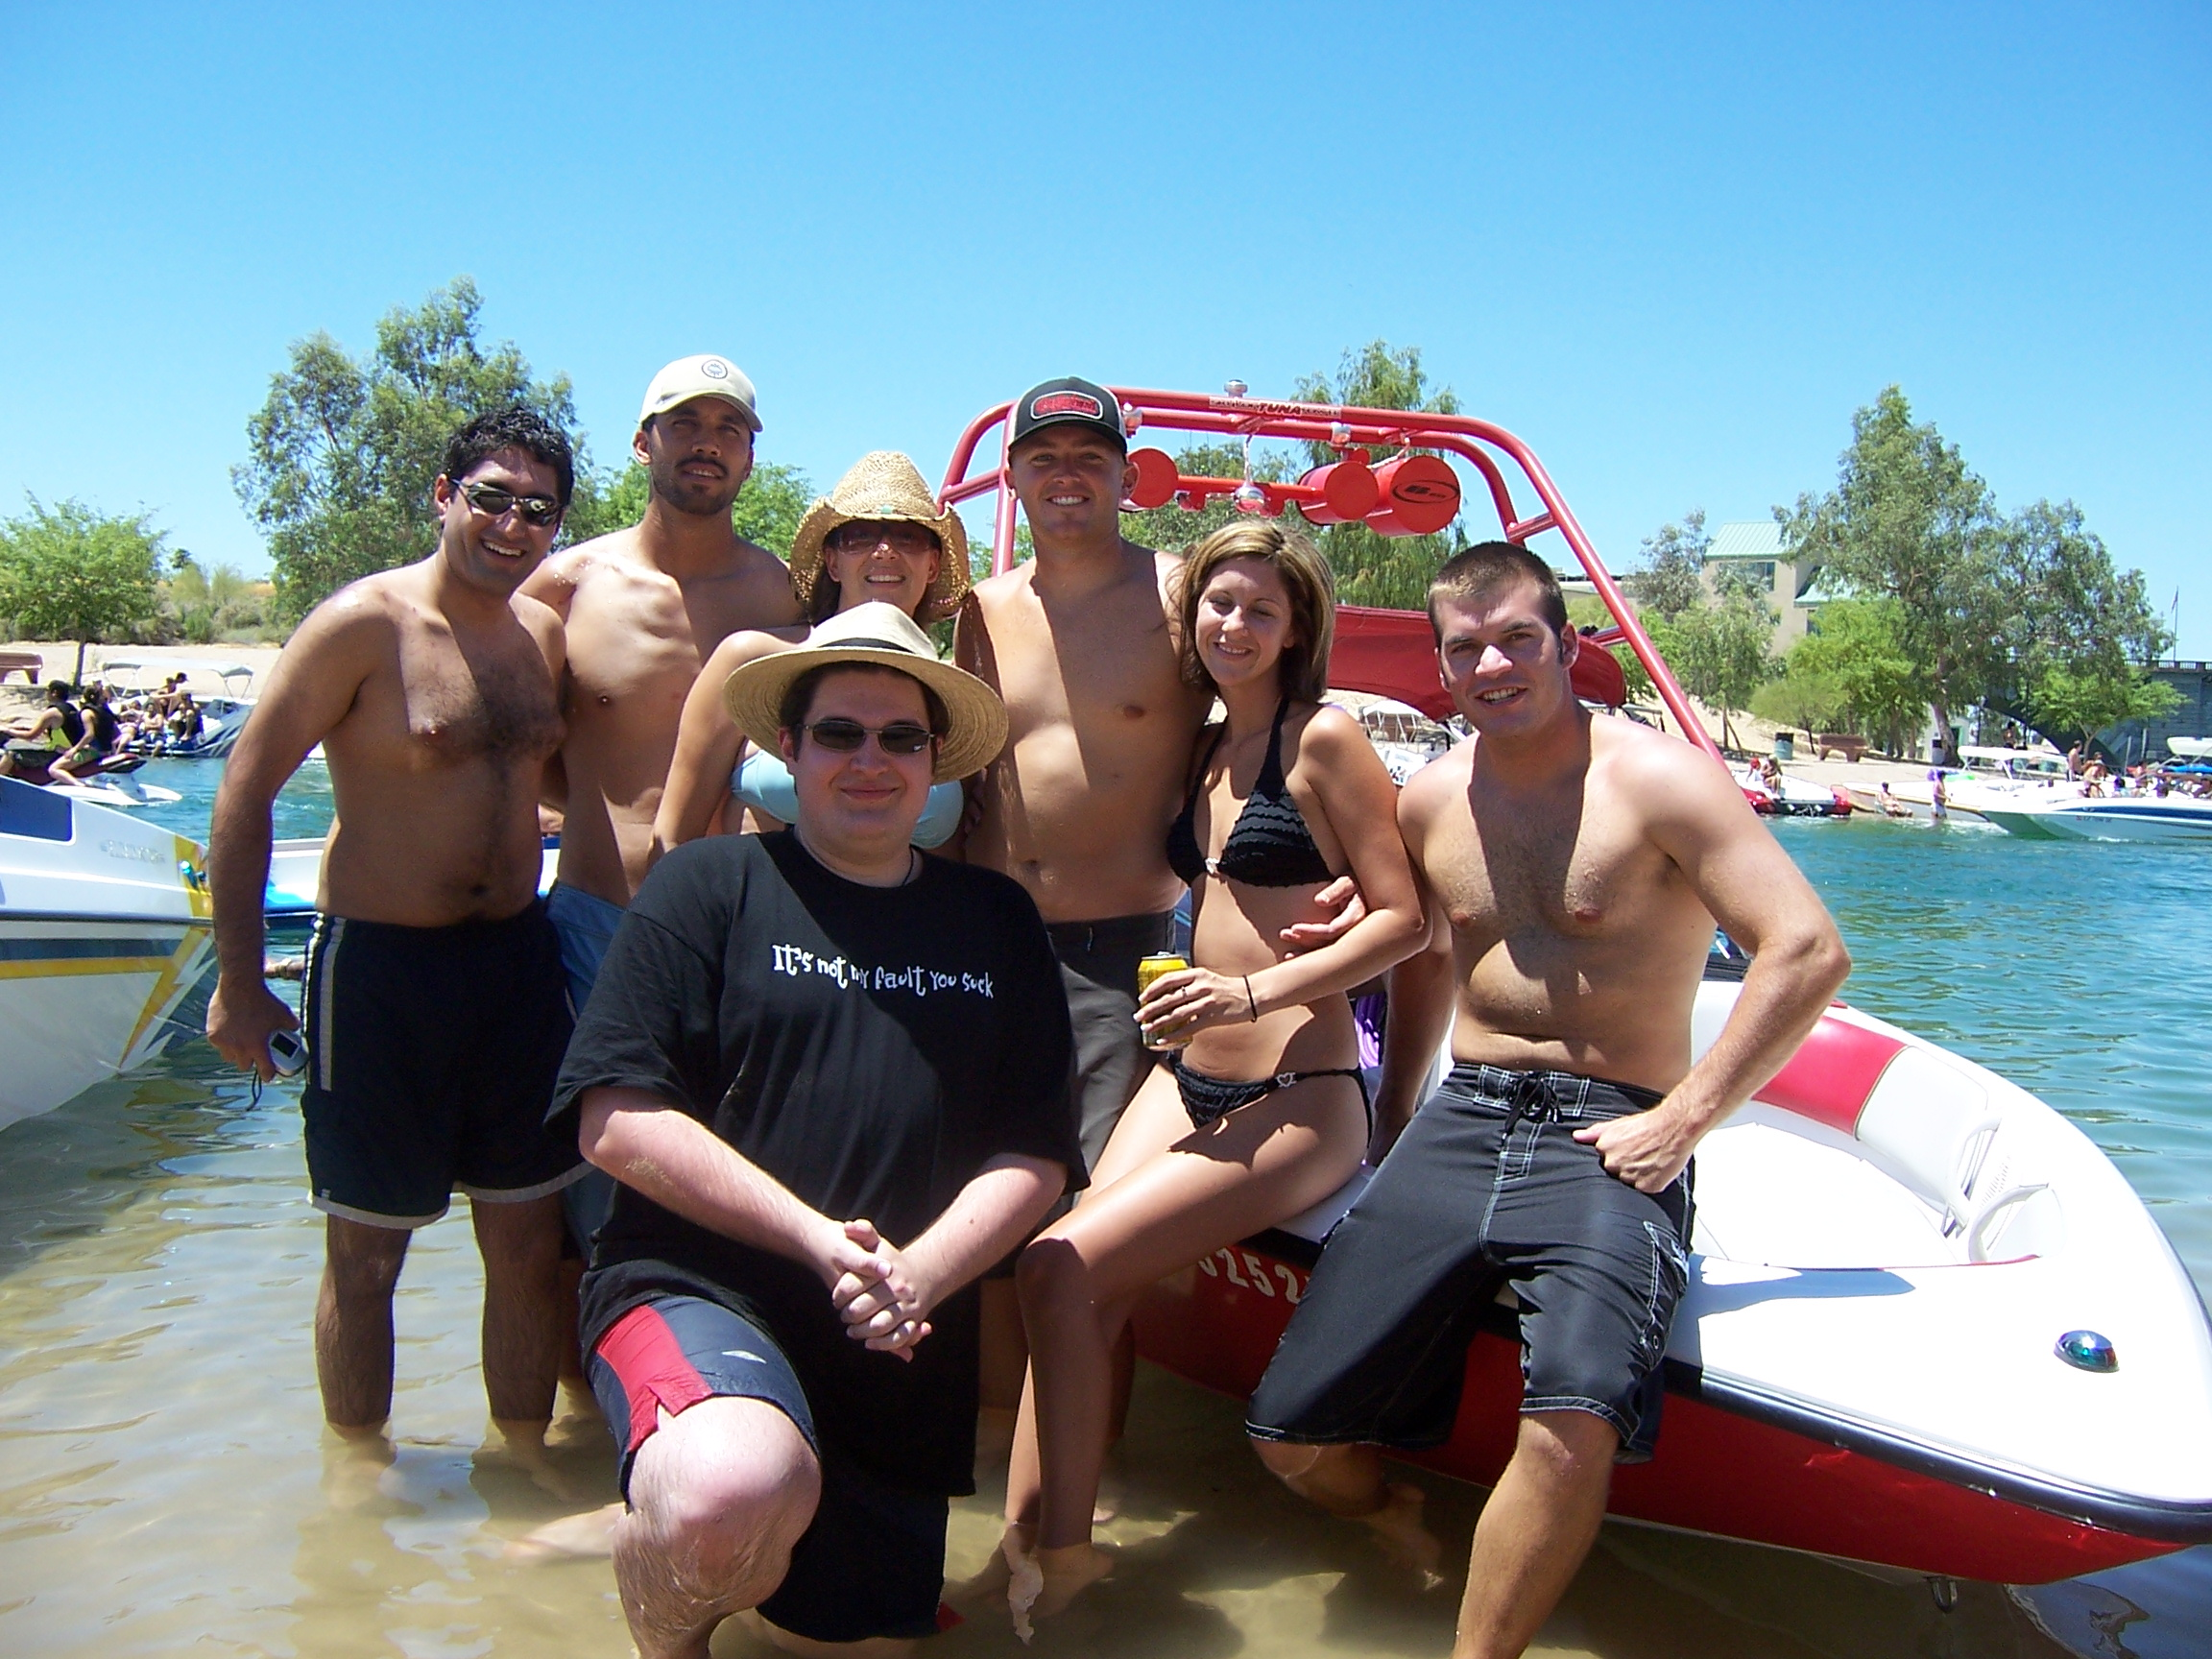
\includegraphics[width=\textwidth]{gfx/100_1604}\end{center}

We badly misjudge the distance from where we are to our hotel and we insist that our hosts, after having given us so much already, do not need to ship us back to where we started.  ``It's fine,'' we say, ``a nice walk back will be good for us''.  It was no such thing, and we trudge through the closed-down and frankly depressing English-themed plaza.  I'm desperate for the bathroom but they're all locked down.  Onwards we walk, across the London Bridge and onto the large island on which our hotel (and, indeed, a third of the city) stands - albeit some distance ahead.  We don't know it yet, but we've fell foul of the scale spaz once again.

It's our intention to take short-cut by heading into the water past the nearest beach.  The beach appears to be an annex of some caf\'{e} and we wander through it and nonchalantly before wading crossing the burning-hot sand to the water's edge.  We try to follow the waterline but find the way blocked by a massive fence which cuts the water in two; we try to wade out and go around it but there's just no way.  The rocks underfoot are treacherous and the water here is scummy and horrible and we have no wish to submerge ourselves in it and so, defeated, we return to the road.

It's ridiculously hot; the sky is clear and the sun beats down on us oppressively as we forlornly wander up the strangely deserted road in the direction we \emph{think} our hotel is in.  There is nothing to our left and right but dust and sand.  I begin to get desert fever.

After what feels like an eternity we arrive back at our hotel, feet aching and sweating like crazy.  It's way past the time we should have checked out but crafty Imran decides to give our room keycard - which we've held on to - a quick go.  Pay dirt - it opens and reveals a pristine, clean hotel room that only hours ago held our sleeping, drunk selves.  We share a look and answer the unspoken question of ``how far should we push it?'' by immediately dragging some fresh clothes back from the car into the room and showering before hastily clearing out again, literally moments before the next guests arrive (we're packing up the car just outside when they do) to find soggy towels defacing their shiny new room.  Anarchy, man.

We wheelspin outta there like bandits.

\section*{Palm Springs}
We hit the road, leave the town and head south, following the slithering course of the lake on its eastern side past the point where it fizzles out and narrows into the plain old common-or-garden Colorado River.  We follow it to Parker, where it bends west and the road keeps on going due south.  Deep into the badlands it takes us, past miles and miles of nothing but the occasional saccharine billboard.  My absolute favourite is a giant montage of a Star-Spangled Banner with the Rocky Mountains in the background and a Bald Eagle, wings unfurled, hurtling towards the Statue of Liberty.  It couldn't be more American if it had slavery and a Domestic Weak Beer on it - although of course, you can find the Rockies and Bald Eagles in Canada as well.

South we travel until Quartzsite, a deliciously-named town with nothing to offer, before we turn west for the last time and finally cross the Colorado back into California, where the only `Welcome to California' sign we can see has a rather uninspiring representation of the State Flower, the California Poppy.  I'm amused that, with everything this enormous and diverse state has given the world, that's what they choose to welcome visitors with.

Westwards, then, through the Inland Empire and by the time we enter the Coachella Valley (via points on the map enchantingly named Desert Center and Cactus City), it's dark.  We skirt around Palm Desert (wonderfully named and, of course, a rich history of music - c.f. \emph{Kyuss}, \emph{Queens of the Stone Age}...) and exit the highway at Palm Springs before immediately getting lost among the manifold golf courses, country clubs and tennis courts.  Thankfully the city is laid out in a perfect grid and we eventually check in at the Wyndham.  The lobby is very light and airy and, for some reason we never quite fathom, has a gaudy, multicoloured statue of a goat to welcome people.

It's clear the place was really designed for wealthy people; not the faux-rich of Las Vegas or even the boat-owning menagerie of Lake Havasu City but plain, simple \emph{money}.  The place oozes poshness from its pores, even the boulevards and the roads feel high-class, lined with row upon row of tall, proud palm trees.  It was a favourite retreat of old-timey celebrities and Hollywood personalities (many streets are named for famous people like Frank Sinatra, Dinah Shore and, um, Gerald Ford) and someone tells us this is where our favourite contemporary Heat magazine subjects come to recuperate after plastic surgery sessions.  \emph{Allegedly}.

After checking in, we immediately head out in search of food.  We have absolutely no clue which direction to drive in, so we navigate using only The Force.  It fails us on a few occasions as we end up at dead ends, facing the looming, shadowy western wall of the valley - the San Jacinto mountains, only a couple of miles away.  Eventually we find a Pizza Hut and abase ourselves by entering within.  I assert that, actually, the salad buffet is usually quite good and order it.

I immediately wish I hadn't - it tastes like ass and Imran's massive pizza looks mouthwatering.

We decide to retire and head home.  Our room has a door separating it from another room on the other side and we think we can hear ladies' voices on the other side; this turns us into randy teenagers and we immediately hatch all kinds of plans to convince our counterparts to unlock their door so we can communicate - absolutely none of which we follow through with.  Eventually we settle for unlocking our side and then we catch some zeds, fantasising that perhaps they will investigate their door, notice us on the other side and, well, romance will ensue.

We sleep like babies.

\chapter[Palm Springs]{Sunday, June 5:  Palm Springs}
Indeed, we sleep until midday the next day.  We don't really have an agenda for Palm Springs and so we look to our map for inspiration.  Our first port of call is the city centre, it's an easy drive away and we decide to look around the shops.  Imran munches his leftover pizza from last night and I decide to grab something from the local Starbucks branch.

Starbucks seems to be the hub of the town and is filled to bursting with preppy, arty types - it seems Palm Springs has its fair share of artiness and, surrounded by such natural beauty, who can blame it.  The mountains climb up impressively at the edges of town and we're not all that far away from places like Joshua Tree and the high desert.  They have also solved the issue of midday heat, through which we are now trudging, by installing vapourising water sprinklers into the canopies of the footpaths which they turn on during the hottest periods.  We walk down the main drag through fine mists of perfectly cooling moisture but, it being so hot, you never actually get wet.  Ingenious.

There's not a lot to tickle our fancy; we give the Desert Museum (actually an art museum) a miss but duck into an art shop anyway.  There's some wonderful paintings but they're all way out of my price bracket so, instead, we run across the busy road and into Staples - yes, the stationery store.  I'm eager to spend money on \emph{something} and so, out of all the art and desert paraphernalia available to me, I buy... a USB memory card reader.  We wander back to the car, shunning (citing tiredness) the famous cable car ride to the top of the mountains and forfeiting the apparently breathtaking views over the entire valley.

\begin{center}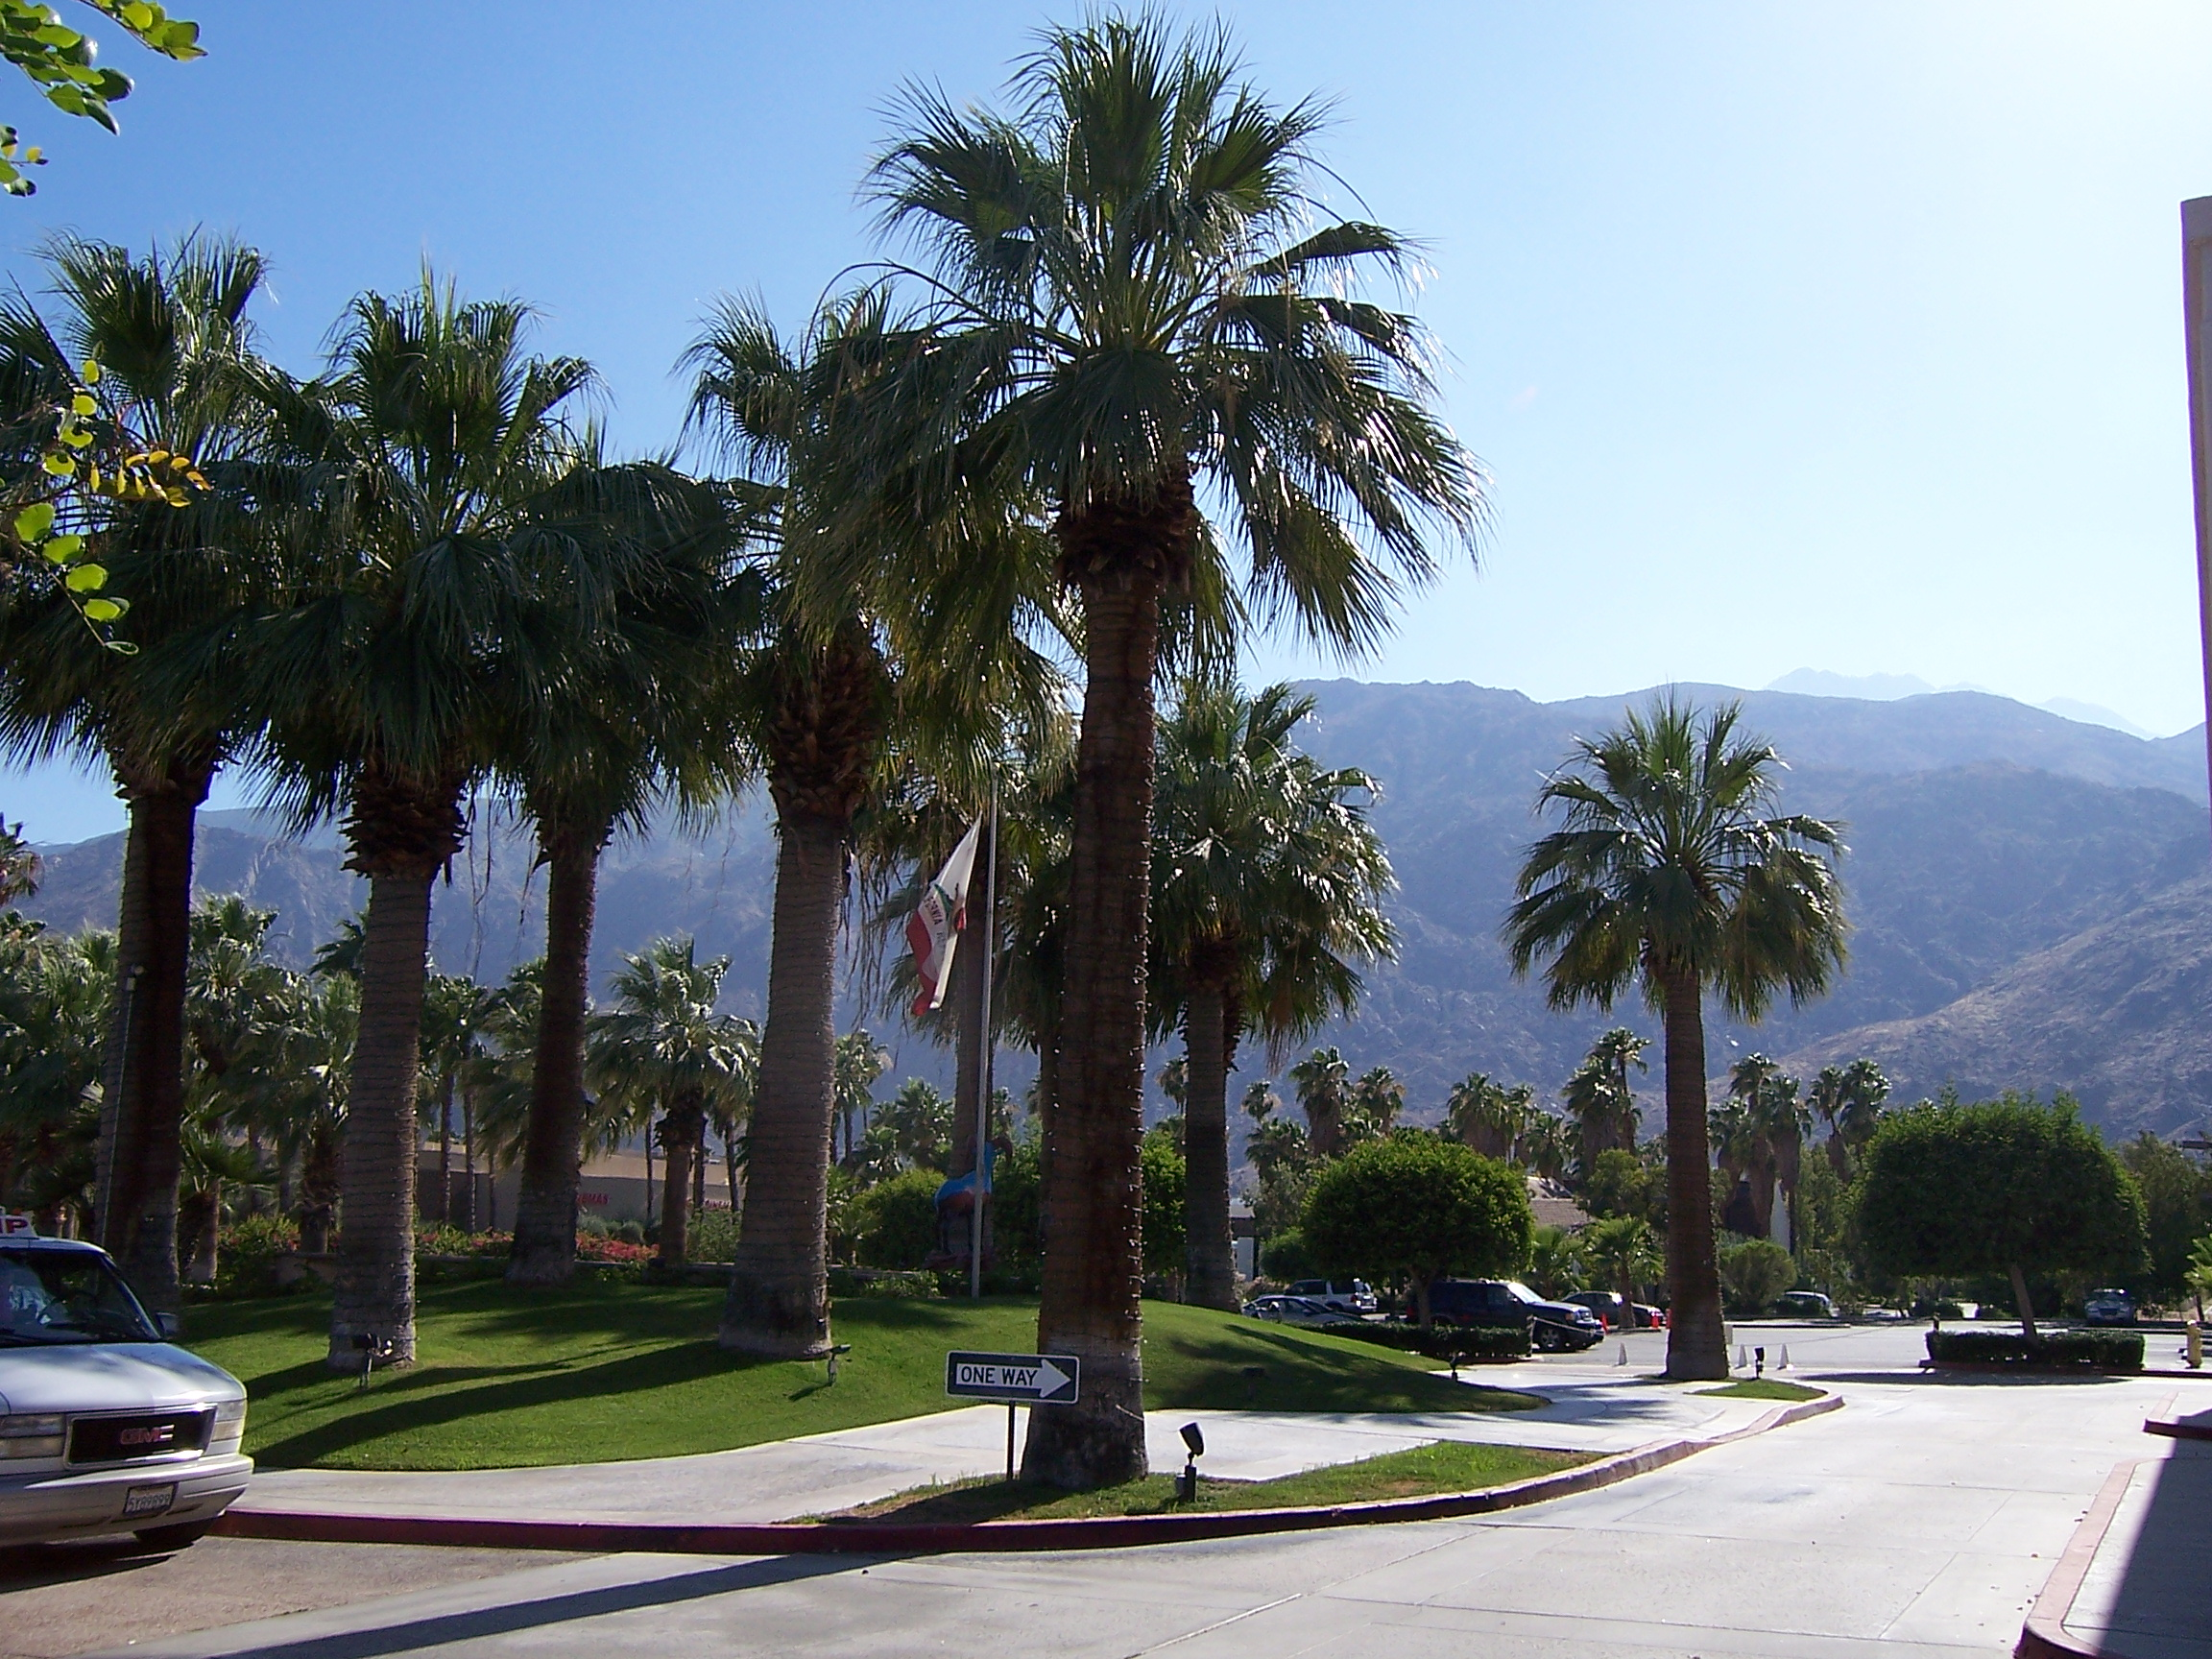
\includegraphics[width=\textwidth]{gfx/100_1625}\end{center}

Our maps and literature point to the existence of some Native American land nearby, on which is an outlet mall and, annoyingly stereotypically, a casino.  We resolve to find it and drive out out of the town, north-west, on Palm Canyon Drive. We're only a short distance outside of town, through, when we see something that blows our mind.

There is a small road leading to a small, deserted railway station.  We drive to it and park up, disembarking and walking a short distance into a sun-blasted dusty plain to the west.  In the field are hundreds and hundreds of wind turbines - more wind turbines than we though could possibly exist in the world.  The dust and the noise is \emph{astonishing}.  They stretch west as far as the eye can see, and they're \emph{tall}, majestic even.  The wind gusts at unbelievable speeds, making our movements sluggish and even threatening to tear the clothes off our backs.

\begin{center}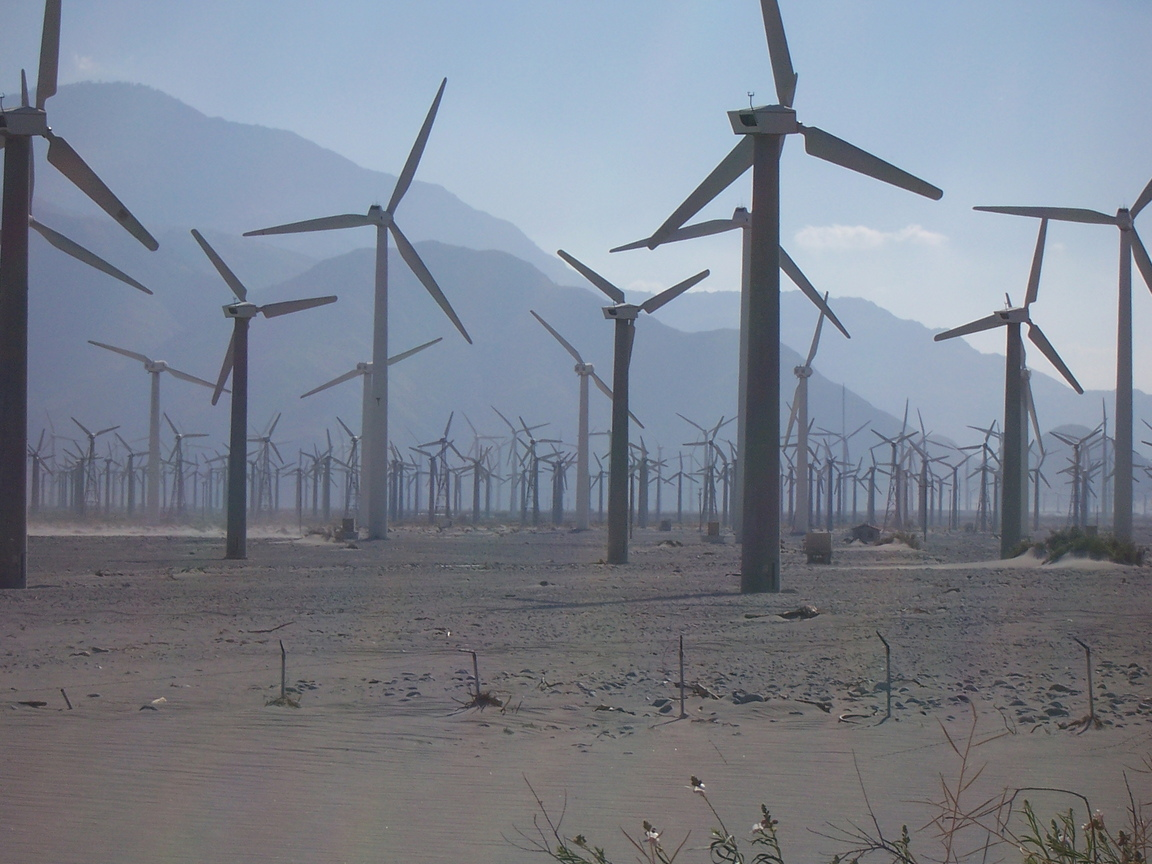
\includegraphics[width=\textwidth]{gfx/100_1636}\end{center}

Imran and I are fascinated and even a little scared of these massive, powerful structures.  We dare each ether to get close to one and eventually pluck up the courage to tentatively touch one, recoiling as though it could electrocute us.  At their bases they are easily wide enough to swallow up our car.  Occasionally the wind drops, the dust stops its relentless billowing and we can see them covering the hills and mountains that surround us.  Again the connection to Kyuss as I recall the striking album artwork to their \emph{Sky Valley} album - that of a lonesome turbine in the desert.  I convince myself I can feel, out here, the force that drove the creation of the music that influenced me so much.  I also convince myself that photos for the album art were taken at this place - it's not improbable - and feel a little like I'd touched something `famous'.

After a long, exhilarating while, we head back to the car and the road, eager to find this supposedly massive shopping mall.  We travel west on Interstate 10 for a long time, seeing nothing but signs promising the world but pointing to nowhere, before thinking that we may have been conned and so end up doing an enormous U-turn.

\begin{center}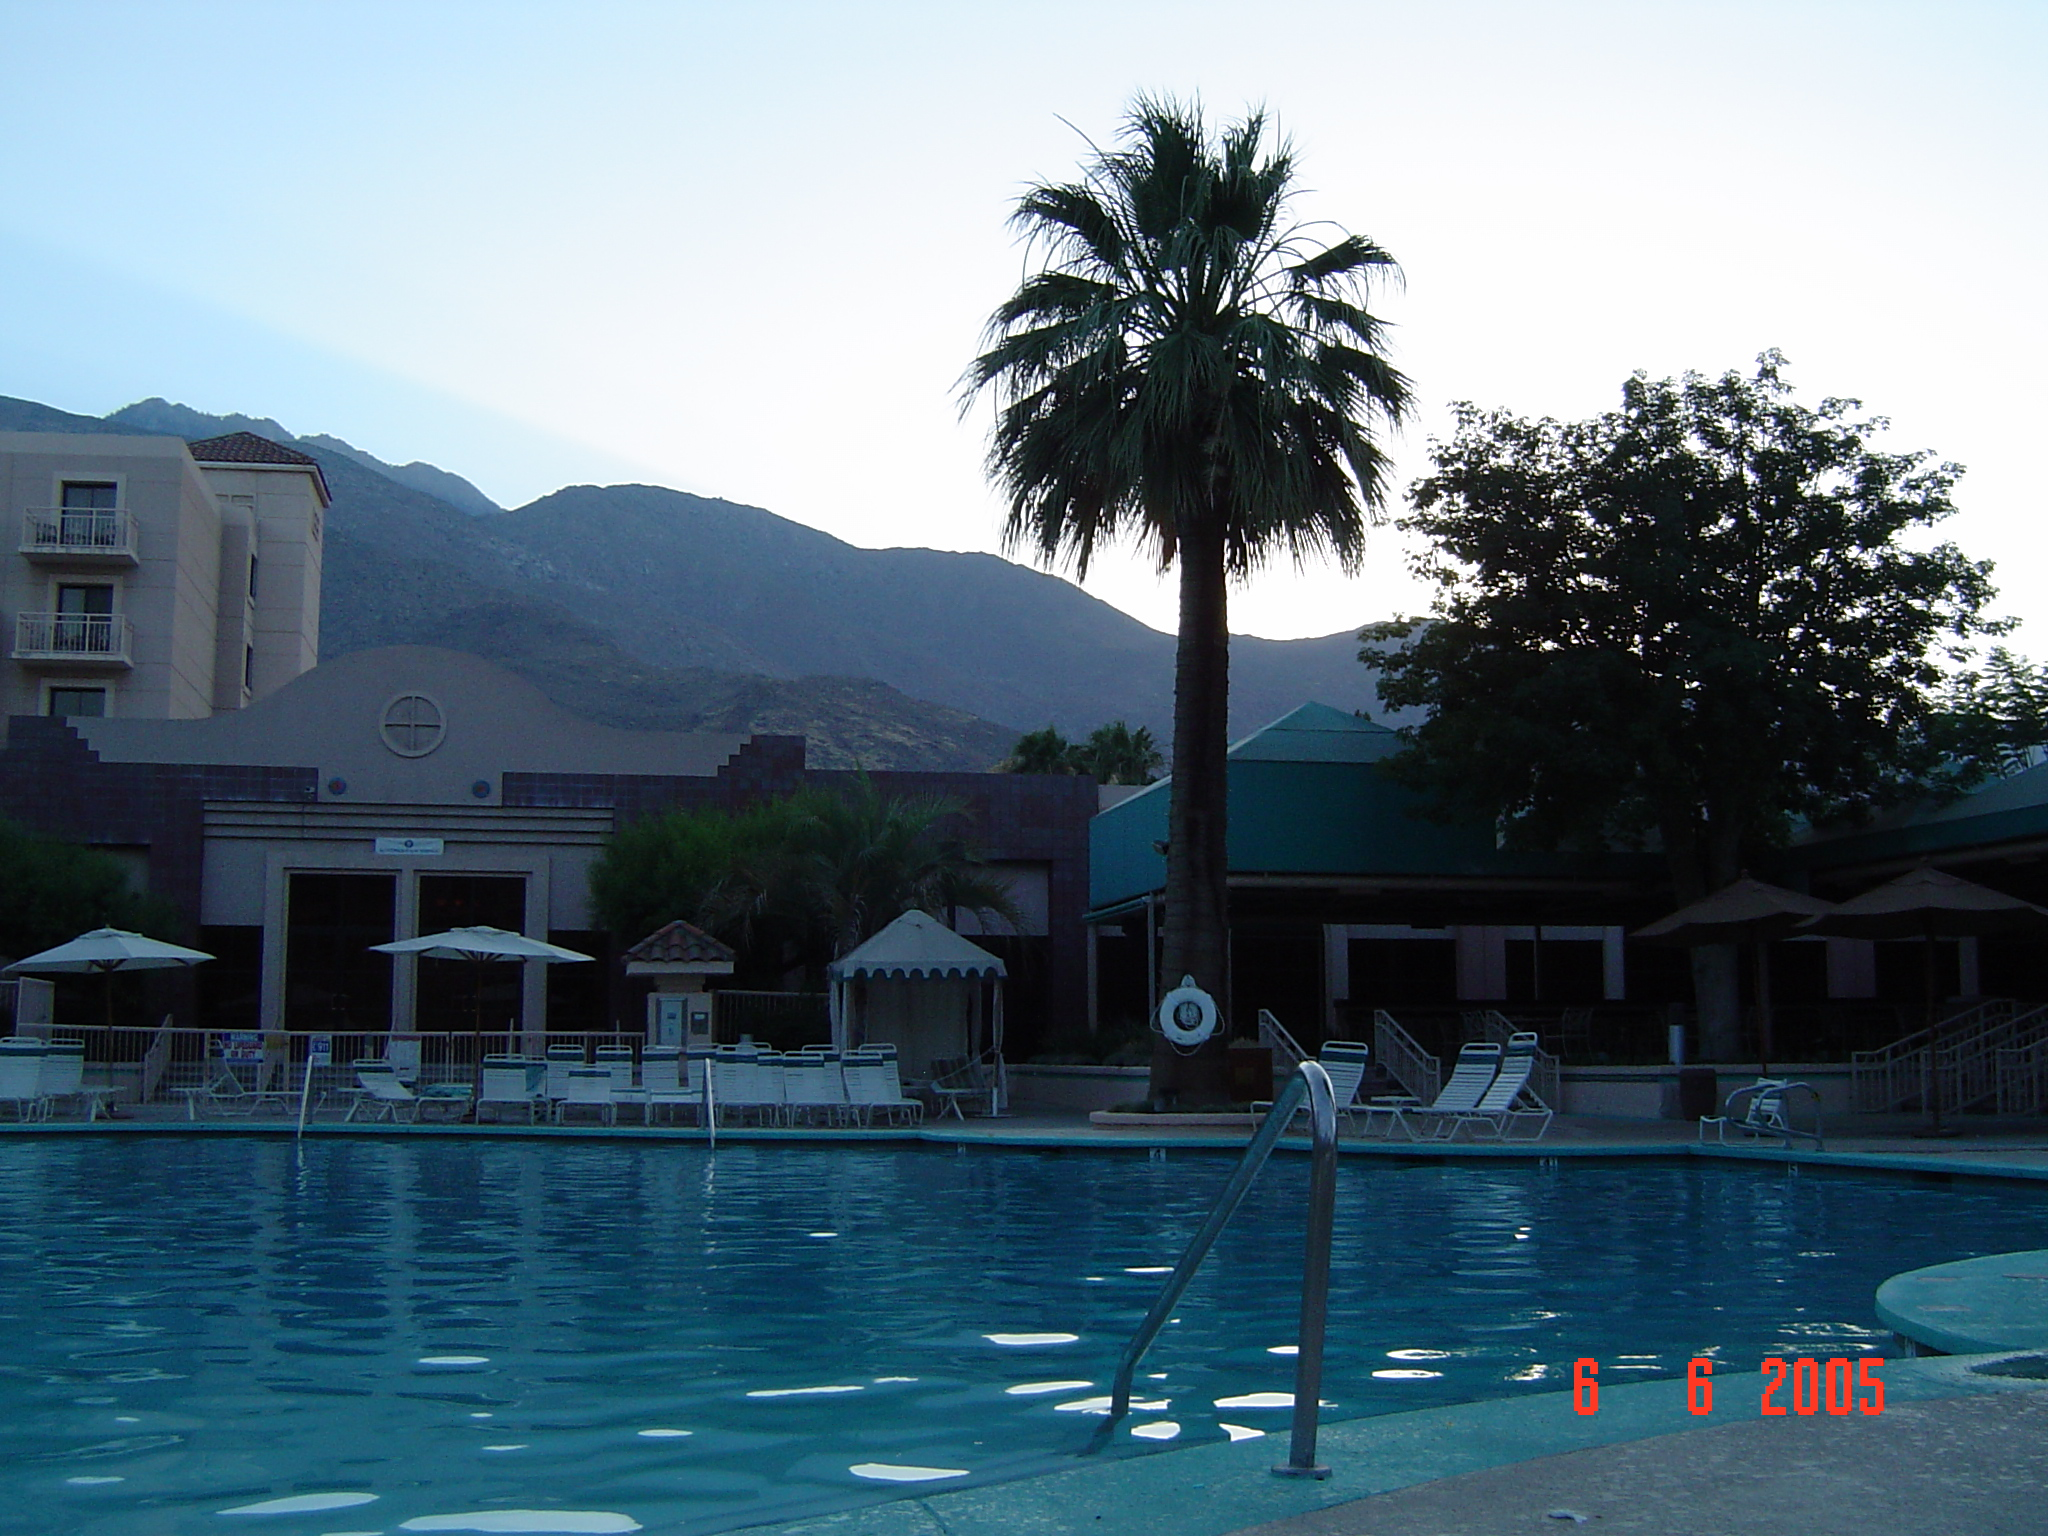
\includegraphics[width=\textwidth]{gfx/palmsprings_pool}\end{center}

By the time we arrive back at the hotel, it is about 6.30 in the evening.  The sun is still up and it's still very comfortably warm.  We decide to shake the desert dust off ourselves by taking a swim in the hotel's outdoor pool, which is large, surrounded by palm trees and deserted.  Just over the rooftops we can see the encircling mountains scraping the blue skies.  It incredibly peaceful and I lie on a sun lounger, close my eyes and listen to my new favourite album, Nine Inch Nails' \emph{With Teeth}.

We wander back into town, this time on foot, in search of food and entertainment.  We find a pleasant restaurant and eat a delicious Mexican meal at our tables on the pavement.  Afterwards we wander up and down the dark, disappointingly empty streets before finding ourselves at what feels like the only bar in miles.  It is called the `Village Pub'.  It takes us a little while to explain to the dullard doorman that a UK Passport really \emph{is} an official proof-of-age before he lets us in and, once we're in, we immediately realise it wasn't worth the effort - what little people there are inside are keeping themselves firmly to themselves.

Maybe our experience at Lake Havasu spoiled us, but with little chance of good company and social interaction, we drain our beers quickly and walk back to the hotel.  We spend a little while in the hotel bar but fare little better and so we resolve, instead, to get drunk - which we barely manage.

When we finally take the lift back to our floor, we're met with a clutch of ladies in the corridor outside our room - they are laughing and frolicking and seem to be having a good time.  Imran and I share a look that says `jackpot' and we introduce ourselves.  We would very much like to be a part of their party and try to strike up a rapport but find it very difficult for some reason.  In the end the exertions of the day take their toll and we say our goodbyes before drifting off to sleep to the sound of giggling.

\chapter[Palm Springs -- Los Angeles]{Monday, June 6:  Palm Springs -- Los Angeles}
For the first time in ages, we get up early and, after a deli breakfast, hit the short stretch of blacktop that links us to our final destination, the City of Angels.  It doesn't take us long to run through Riverside County and eventually terminate at Anaheim.  We're staying at the Sheraton and, for the first time, we find it without incident (it being conveniently located just off the Santa Ana Freeway).

En route we discuss our plans for the coming few days.  It is our firm desire to go drinking and clubbing and try our best to meet women and party.  At the checkin desk, Imran startles the young lady by insisting she tell us `where is good to go in Los Angeles'.  She has no answers for us, I imagine because we have confused it with an average, regular-sized city.  You see, the problem with Los Angeles is that it is absolutely \emph{enormous}.  It is criss-crossed with motorways and yet it still takes at least an hour to get from one side to the other, travelling at speed - the same time it would take to cross half the width of England.

Our plan for the remainder of the day is to conduct a circumnavigation of the city and, since we're starting in Orange County (recently brought into the public focus by \emph{The O.C.}, which I'd never seen), we elect to hit up Newport Beach.  I'm told it's where all the cool posh kids hang out and it should be \emph{crawling} with hot young ladies, just like on the telly.  It's a short drive due south and we arrive without drama for our first taste of the mighty, magnificent Pacific Ocean.

I take off my shoes and socks and wade into the ocean up to my thighs to commune for a while, finally feeling the warm, soothing waters and feeling right at home.  I've been in love with the Pacific and, indeed, this whole city, for years now - hearing it in music, seeing it in films and in books.  It is wonderful to finally be there (although of course we'd seen it back in San Francisco) and we boggle at the idea that, half the world away in this direction, is Japan.  My cool sunglasses - the cause of embarrassment a lifetime ago and four hundred miles north-west - are perched on my head.  It is the last time anyone sees them.

\begin{center}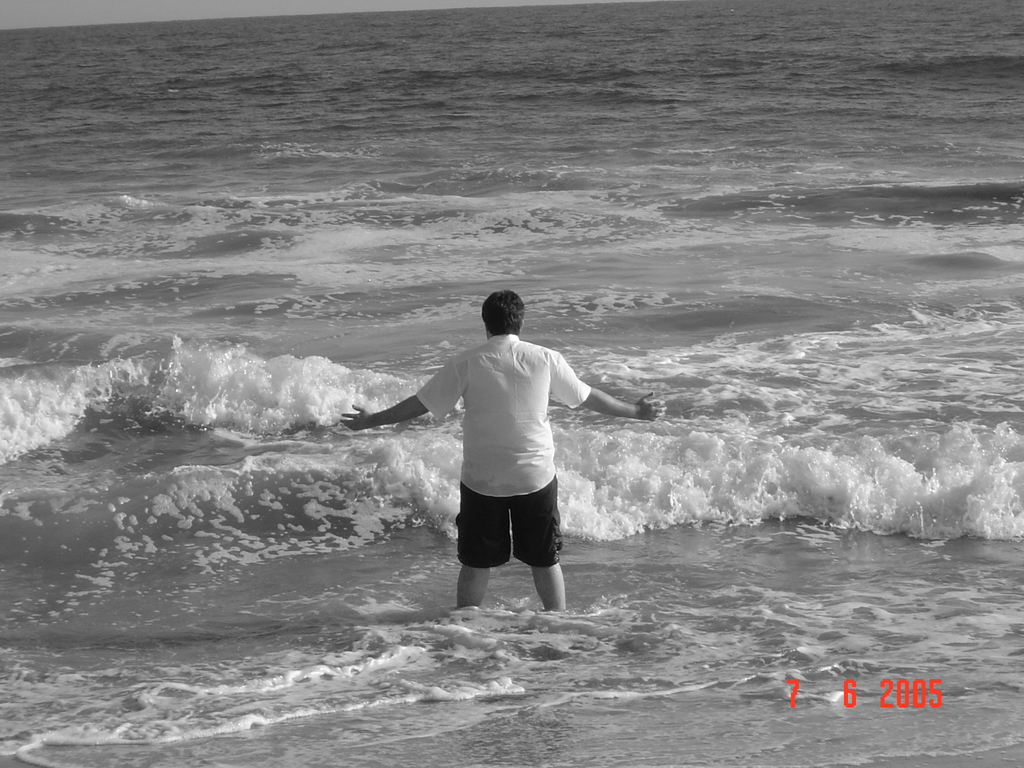
\includegraphics[width=\textwidth]{gfx/pacific}\end{center}

We see no famous people filming teen television dramas, no hot ladies and, indeed, no-one at all and so head back to the car and up Route 1 - the Pacific Coast highway.

What we did see \emph{lots} of were oil derricks, oil pumpjacks (`nodding donkeys'), oil tanks, oil-related structures and devices of all kinds.  We look inland as we drive north and, on the wasteland patches, there are pumpjacks.  We cross over a marshy area around Seal Beach which is littered with the things.  We even spot a `desert island', complete with palm trees, just offshore which, upon closer inspection, is a tiny oil drilling platform which is simply \emph{disguised} as a desert island.

\begin{center}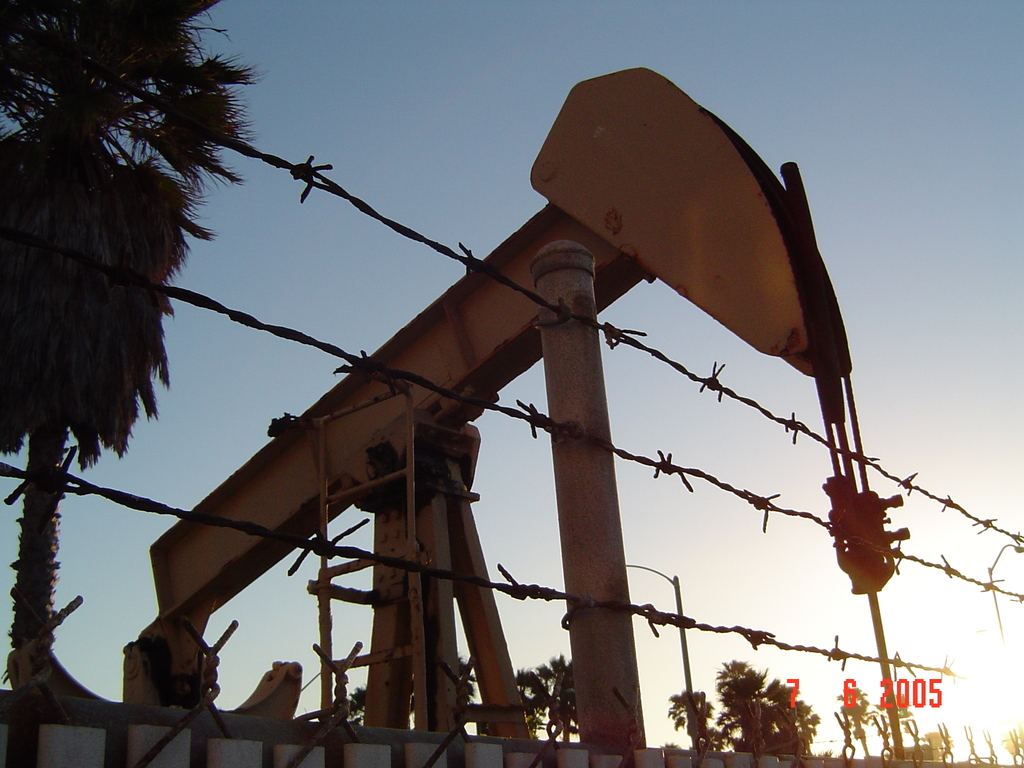
\includegraphics[width=\textwidth]{gfx/pumpjack}\end{center}

I find the sight of them repellent.  Just north of Seal Beach we pull into Taco Bell for a bite - another quintessential American thing that I was eager to try - and in the \emph{car park} they had a pumpjack in a fenced-off area.  We stare at it for a long while, its hypnotic, ceaseless, rhythmic motion invokes dark thoughts in me: it really does feel like the Earth is being `violated', and my lefty Greenpeace rage builds when I realise that this pump (surely \emph{all} such pumps) will simply \emph{never stop until there is nothing left}.  It makes me feel sick.

A passer-by sees us and clocks our dumbfounded looks at the sight of this ethically-questionable enterprise in a restaurant car-park.  He simply says ``well, for 500 dollars a month {\footnotesize [or something]}, you'd have one in your garden, too''.

I try to cure my sickness with a Taco Bell taco meal.

I fail.

We drive on, into Long Beach and Los Angeles County proper, where we begin to learn the difficult reality that Los Angeles as we know it actually a massive network of \emph{eighty-eight} cities and city-sized entities over an area of \emph{five hundred square miles}.  The possibility of us getting around the entire city is rapidly fading along with our remaining daylight.  Instead we turn due north and try to get at least as far as Downtown but, alas, our map fails to accurately represent the sheer complexity of the road network and we end up getting just a little lost somewhere around the industrial, shipping and rail yards.  We see signs to Compton which, on our handy tourist maps, joins Inglewood, Wilmington and bizarrely, chunks of Downtown in the dubious honour of being marked by a red square and a note saying `Warning: Do not enter these high-crime areas'.  We recall a stark warning given to us by someone at Lake Havasu:  ``basically, if you go to Compton and you're white, you'll actually be \emph{killed}''.

Instead we find ourselves passing some `authorised personnel only' signs.  Imran and I both share an inexplicable desire to be where we're not really allowed - airside at airports, stood on the tarmac of motorways, that sort of thing - and so we were eager to get up close and personal to some heavy container ships somewhere in the Port.  As we drive around we pass a railway crossing and some crazy industrial buildings; near the crossing is an enormous pipe or valve assembly with a wreath draped around it.  We imagine that some poor schmo met his or her end here, and take pictures before carrying on.

A minute or two later we hear a train's horn hooting and immediately realise that, if we sped backwards, we might be able to beat the surely enormous freight train to the crossing, set ourselves up and take some fantastic pictures.  We burn rubber back down the road to the crossing, by now tingling merrily, warning all and sundry to expect a mile-long behemoth filled with freight from every corner of the globe.

The train comes lumbering towards us and we begin snapping away, high-fiving at the spectacle and our good fortune.  We're certainly trespassing, but my fear has melted away at the sight of this mighty machine, undoubted bound for somewhere mind-bogglingly far away.  After our journeys we feel a sort of kindred with it.

Then the fear returns - the driver has seen us and, as he rolls past, he leans out of his window, shouting and waving his arms.  We realise that we look a little bit like, well, terrorists.  We share a look and slowly start to pack our cameras away, aware that the driver is at the very best calling the site security and, at the very worst, is calling the Guantanamo Bay Snatch Team.

Then, something we most certainly did not expect to happen:  The train stops, shudders for a second, and begins to \emph{reverse}.  I didn't even know those trains \emph{could} reverse.  Somewhere, a mile down the track, some very bemused freight yard workers are watching the last carriage come back towards them.

``We're fucked'', Imran whispers, and we both swallow and prepare to leg it.

The driver re-appears, leaning out of his window.  He waves madly.  We soil ourselves.

``Hey guys!'' he shouts.  ``Take some pictures!  I love getting pictures of me in my shit!''

We're gobsmacked at this simple display of friendliness and could never imagine anything like this happening in Blighty.  We happily oblige the man.  He poses for us, leaning from his train with his arms in the air and we try our best to capture him, his engine carriage and his payload in the inky blackness.  He tells us his name is Eric and scrawls down his address on a piece of paper (a hotel somewhere in the city), asking us to get the photos printed and mailed to him within 48 hours because he must then drive his train to... I dunno, Poughkeepsie, New York.

We promise to do just that and, with a final cheery wave, he starts his engine and hauls onwards.  Imran looks at me and says ``that was fucking weird''.  I nod.

It's now almost nine and we decide to head back to the hotel with all speed which we achieve courtesy of the Santa Ana Freeway, which we reach via a heart-in-mouth trip around the periphery of Compton.  Just before our exit, though, is a giant 24-hour Walmart which we decide to check out, primarily to make prints of Eric and his train on the DIY photo printing machines.  Alas, we're saddened to find that all of the pictures are really very dark and/or blurry, so much so that we decide it would be less embarrassing to send nothing at all.

Sorry, Eric.

After freshening up and a swift bit of detective work with the girl at the hotel front desk, we learn that there is an area of the right-next-door Disneyland called `Downtown Disney'.  For some inexplicable reason, the name evokes images of a dark, seedy, quite \emph{adult} venue (...in a children's theme park...) and so we elect to go there in search of... nightclubs.  After all, surely after a day of taking the kids around, there'd be somewhere for the grown-ups to relax, right?

What we find there is a single, awful bar where we both drink a single, awful beer before being thrown out - it's closing time.  We are faintly depressed.  It's night time in \emph{Los Angeles}, for Heaven's sake, we want to party and we're being thrown out of Disneyland.  Something has gone very wrong.

It gets worse when we can't find anywhere to buy a bite to eat.  Surely we should be falling over 24-hour diners and coffee houses?  We trawl up and down the roads desperate for a KFC before finally deciding that the city of Anaheim is \emph{rubbish} and settling for the single place we can see that will serve us - a fast-food burger joint called \emph{Carl's Jr}.  We order up some meal deals and head back to the hotel to forlornly eat them before finally giving up and calling it a night.

Better luck tomorrow.

\chapter[Los Angeles]{Tuesday, June 7:  Los Angeles}
We sleep until midday.  Before we left the UK, we had made a checklist of places we really wanted to see - the usual suspects of Santa Monica, Hollywood and Beverly Hills but also the Hollywood Hills and the San Fernando Valley.  Again we plot a circuitous route and hit the highway.

It's 2.30 before we eventually get to Santa Monica.  We spasm around a bit looking for parking before sliding in next to an enormous 4x4.  As we get our parking ticket we spot the owner heading for and getting into it.  I am absolutely sure it is Brandon Boyd, front man of \emph{Incubus}, but before I can simper over him and shake his hand, he takes off.  I am flushed with coming so close to a `celebrity'; Imran shakes his head in disdain.

We head onto the beach.  As usual, it is a glorious day but the area is oddly empty (I suppose it \emph{is} mid-afternoon on a weekday).  After a joyous plodge in the enticing water we take a quick walk up and down the boardwalk, dodging skaters and bikers and dog-walkers galore.  A few hundred metres north of us is the Santa Monica pier but we decide not to waste time heading onto it - we have places to be.  We note a dishevelled hobo skulking around on the sand and are bemused at the juxtaposition.  We take pictures of him and move on.

\begin{center}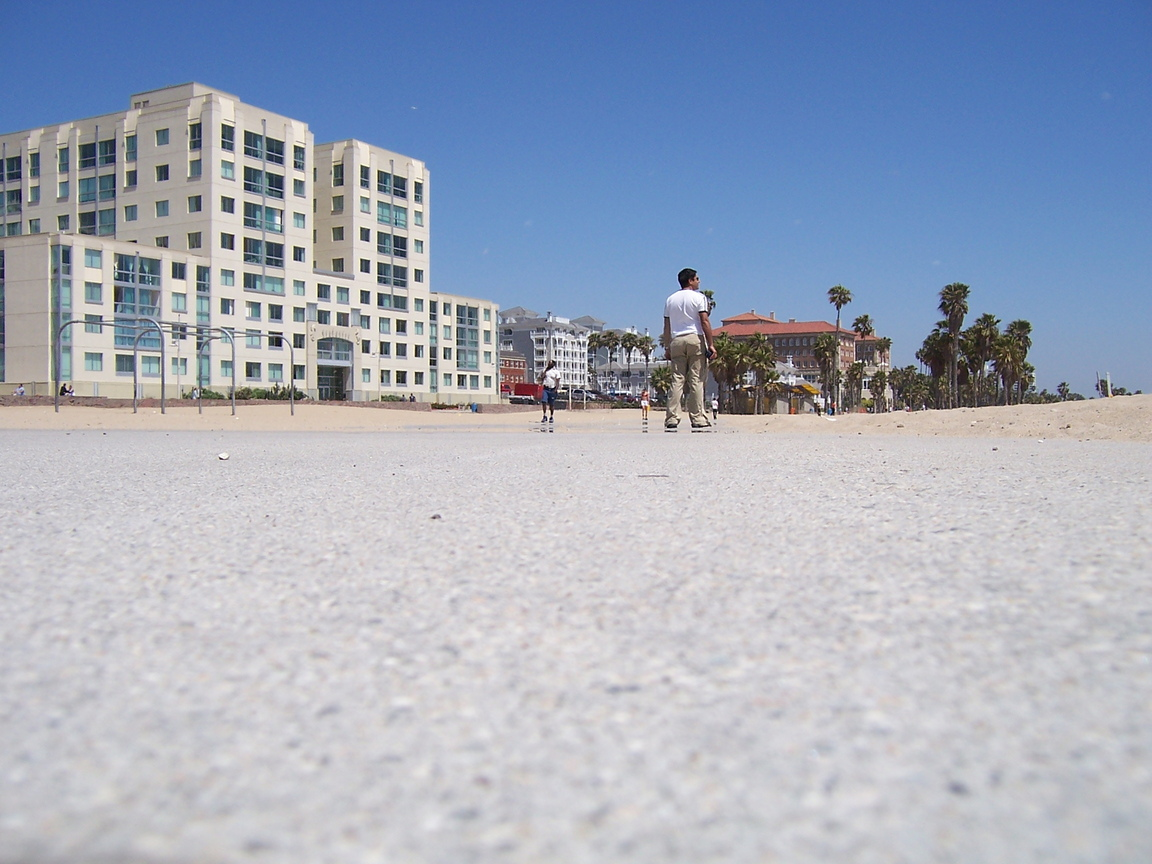
\includegraphics[width=\textwidth]{gfx/100_1735}\end{center}

With Sheryl Crow running through our heads, naturally, we head up Santa Monica Boulevard, snapping pictures out of the car window like a pair of really rubbish gangsters on a drive-by.  Annoyingly there's not much to see and before long we turn north onto the 405 in order to hit the Valley - after a minor whistle-stop tour of Bel Air.

We drive up into the hills and back down again before turning off and finding ourselves at Sherman Oaks, whereupon we decide it's time to park up and grab a bite to eat.  Bizarrely, for such a wide and busy road (we're on Ventura Boulevard), there are parking bays and meters on the sides.  Stopping, getting out and crossing the road feels like a suicide mission, but we give it a go.  There's a large shopping area on the other side and so we head into it, spending a lot of time browsing the Stateside equivalent of HMV.  By chance I find the first, hard-to-get Kyuss album, \emph{Wretch}, which I eagerly purchase.  Imran and I unwind over a coffee at Starbucks before heading on.

With the awesome music playing we carry on east.  We are as far south as you can be and still say you're in the San Fernando Valley (which, in case you didn't know, is where most of the action you \emph{think} happens in Hollywood \emph{actually} happens - it is also, of course, the `pornography capital of the world') and before long we have driven all the way though Studio City, past Warner Brothers and emerge into Hollywood.  We park in some residential street just off Hollywood Boulevard (people actually \emph{live} there!) and check it out.

\begin{center}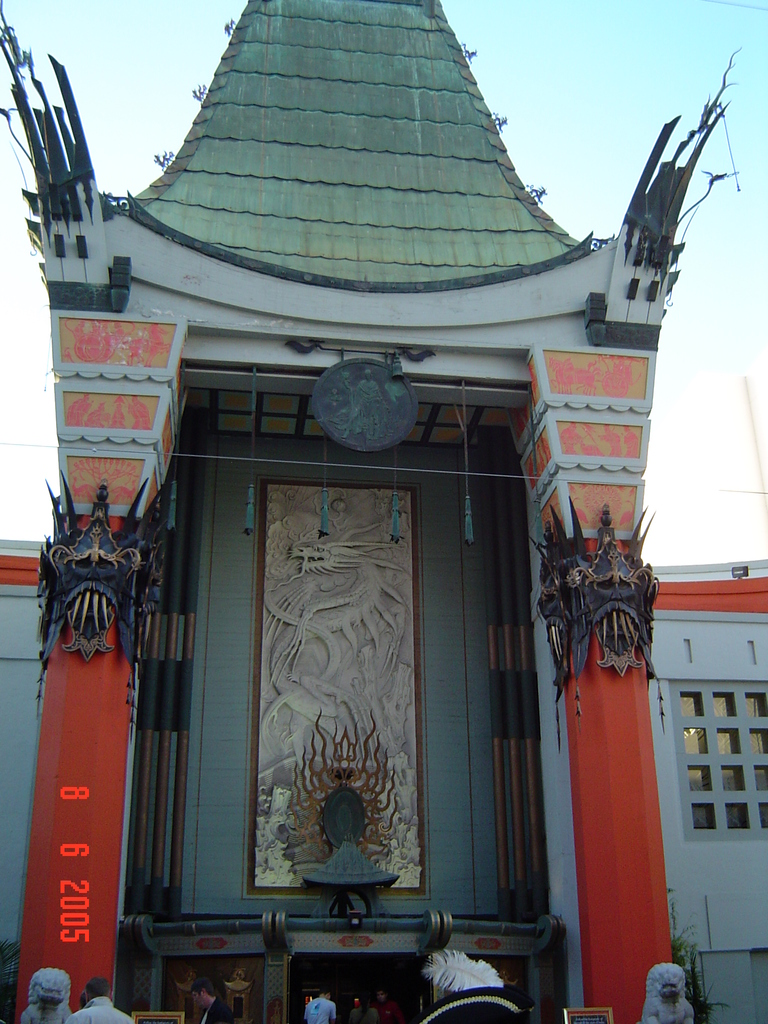
\includegraphics[height=80mm]{gfx/DSC00806}\end{center}

Again, there's surprisingly little to see and do on the boulevard - there's the Walk of Fame, of course - the stars in the pavement adorned with various actors and celebrities' names (we take pictures of the important ones like David Hasslehoff and Samuel L. Jackson); Ripley's Believe It Or Not (we have no idea what this is and avoid it) and Grauman's Chinese Theatre - the one with the cement foot and handprints of various actors and celebrities.

We scoff some greasy kebabs for dinner (a kebab shop on Hollywood Boulevard - classy stuff) and are briefly assaulted by a small man dressed as Chuckie the murderous doll from the \emph{Child's Play} films outside the Chinese Theatre.  We have no idea why he is there - the film isn't playing or anything.  We suspect he is just some dude with nothing better to do.

It doesn't take long to exhaust the immediate attractions and we head off past the adult book stores at the lesser-visited end of the boulevard and up the hills again to the Griffith Observatory.  We're seeking good photo opportunities of the Hollywood sign and figure there'd be no better place.  The view over the entire Los Angeles Basin is certainly majestic and wonderful although, sadly, the deepening dusk acts against us - it's eight PM and we think about heading back home to freshen up.

On the way back down the hill into the city we pass some parkland.  There is a man playing frisbee with his son and their dog. ``See that?'' asks Imran.  ``That shit is the \emph{American Dream}.''

Back at the hotel, we bite the bullet and pay for Internet access.  We do some very careful research online for places to go and party, eventually coming up with a shortlist which does not include Downtown Disney.  We still believe that Hollywood and its surroundings are Party Central and so we choose to head all the way back up north to the Bigfoot Lodge, a short distance east of it and an easy, if long, journey up the freeway from us.  Before we leave, I pack my swimming gear - it's my firm intention to take a midnight swim in the Pacific when the partying is over.

I'm tonight's designated driver and so, when we are parked up and inside the bar, I quaff a Monster Energy Drink and we kick back, relax and make eyes at women - all of whom are able to resist our dangerous, exotic allure.  The inside of the bar is decorated like the a log cabin and for the most part comprises of many booths.  We spend the remainder of the night daring each other to rope in some strangers for company but we can't seem to find an opportune moment and so, besides ourselves, our booth remains empty until closing time.

It's midnight now and I take the wheel, heading west toward the coast - the bar, to Los Feliz Boulevard, to Hollywood Boulevard to, finally, Sunset Boulevard - a place we'd tragically missed until now.  We look on in wonder at the glitzy nightclubs and bars here still packed with people; the Viper Room and Whisky a Go Go pass by in a blur.  After the Sunset Strip we're in Beverly Hills and here the road gets narrower, darker and a \emph{lot} more serpentine.  There are times when it feels like we're driving a rally, the steering wheel spinning almost non-stop, the road sloping up into the hills before finally plunging down to the ocean.

For the second time today we park just south of the Santa Monica pier and step onto the beach for my midnight swim - the fulfilment of a lifetime wish.  There's just one snag - it's completely, pitch black.  We know the ocean is there but only from the sounds it makes.  When we look to our left, some miles south we can see the lights of LAX and the stream of 'planes taking off and landing.  To our right, a few hundred metres up, the pier is shrouded in darkness.  We can barely make out the water violently smashing against the pier supports.  It is surreal and, actually, very scary.  The idea of swimming in that opaque black water fills me with primeval dread and I chicken out.

We see someone who could be some sort of security guard wandering authoritatively over the sand in our general direction - in retrospect such an idea is ridiculous, of course, but at the time we are genuinely fearful of being mistaken for drug addicted homosexual vagrants and taken away.  It is two AM and we beat a hasty retreat.

On our way home we see exactly the sort of thing we'd been looking for last night - an all-night coffee and doughnut joint, which we eagerly pull into.  We step into the place and immediately regret it - the proprietor has the look of a cannibal killer and the only other patron there is a heavily-tattooed biker who stares at us as though he can snuff our lives out through sheer thought alone.  We share a look and telepathically agree that the doughnuts on offer here just aren't worth it, and we leave, hungry.

Thankfully, after we have shunned the freeways and arrived back in Anaheim via countless citylets, we find our old chum Carl's Jr. is open and more than willing to fill the burger-shaped holes in our bellies.  It is three AM and we have burned through an entire tank of gas in a single day just getting around one city (as it happens Los Angeles probably accounted for a quarter of all our fuel costs) - it's just so damn big.  I am still wired from my giant can of energy drink hours earlier but I do my best to recharge for tomorrow.

\chapter[Los Angeles]{Wednesday, June 8: Los Angeles}
After our epic night it's no surprise that we wake up late.  By now our hotel room is a total tip but we're living the rock-star lifestyle, a lifestyle we immediately reaffirm by having a nice, healthy 2PM `breakfast' at the hotel's deli counter bar caf\'{e} thing.

It's our firm desire to take it easy today - we are in one of the world's most trendy cities and it is time for some Retail Therapy.  With fashion on our mind, we wander out to the car park.  En route we pass some sort of unfamiliar lizard and attempt to lure it closer with petals we steal from a nearby flower.  Unsurprisingly, the creature simply blinks at us before running away.

We \emph{are} surprised, though, to find that sometime in the morning, a pretender to our throne had parked their carbon copy of our hearse-like automobile right next to ours - although obviously ours wins out for being a convertible.  What is surprising is that we aren't the only people in the world with such an ugly car and that someone would \emph{willingly} draw attention to theirs.

We point and laugh at it before hitting the road.

\begin{center}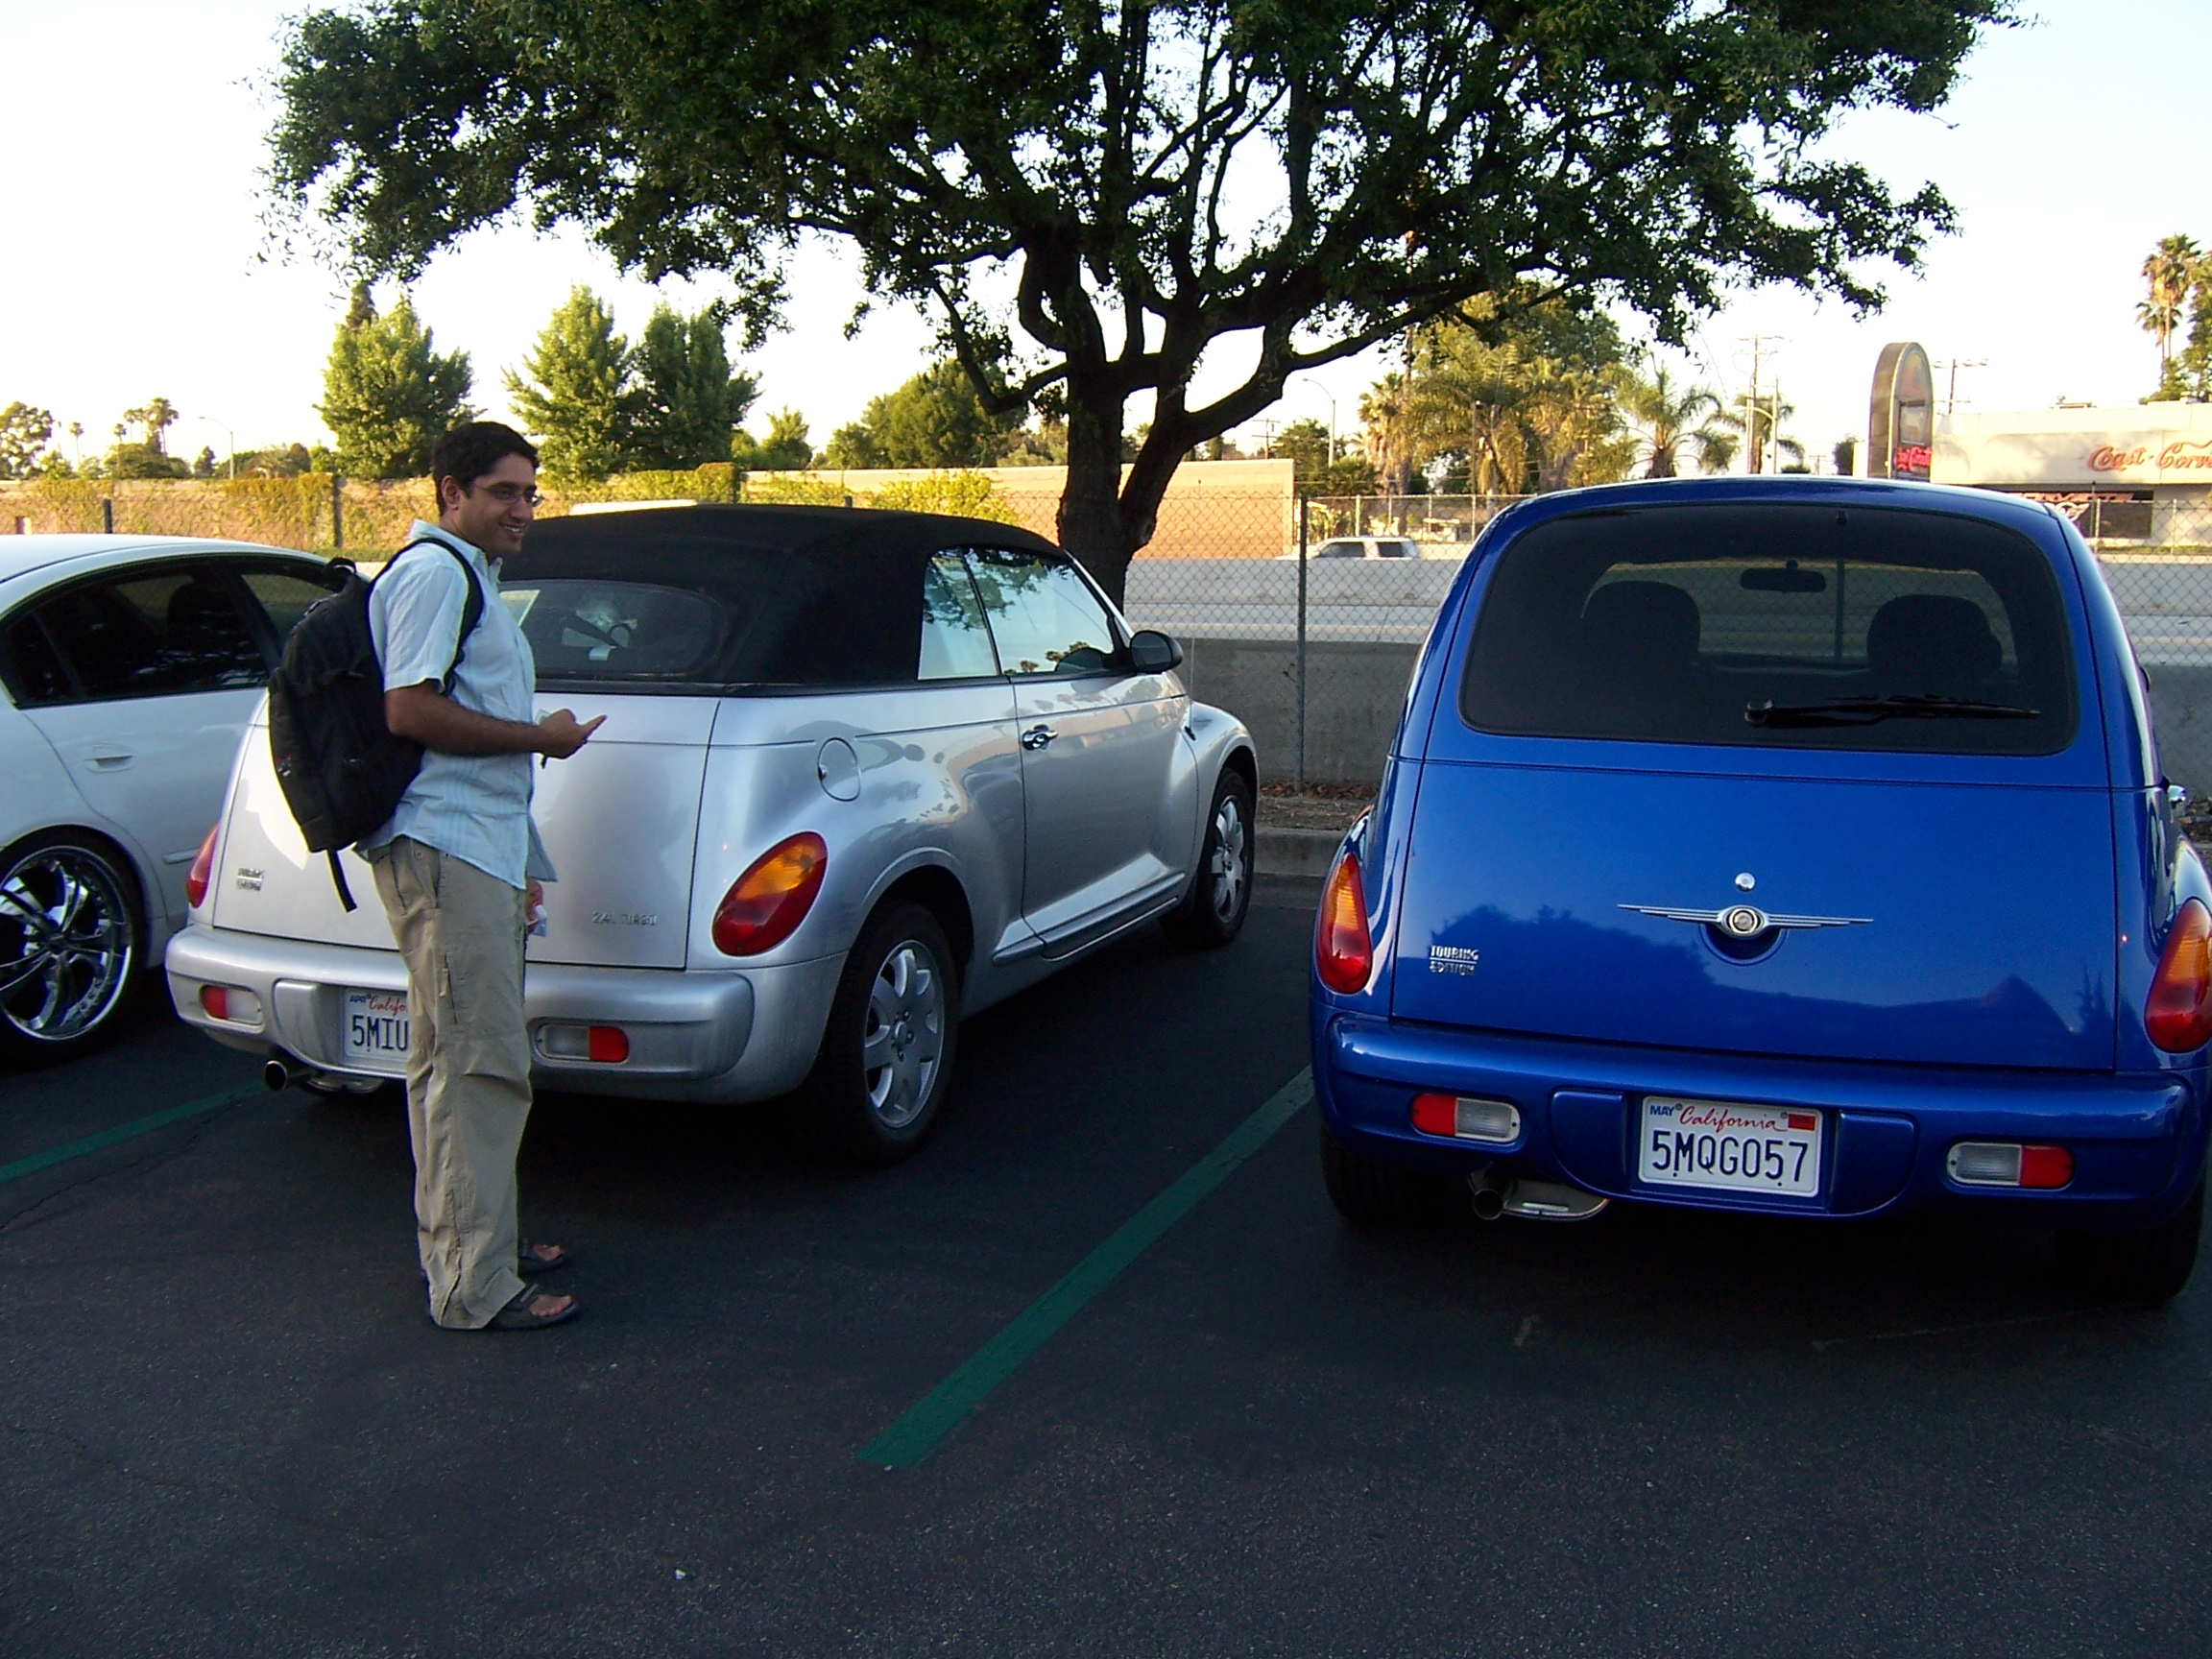
\includegraphics[width=\textwidth]{gfx/100_1793}\end{center}

Having spent the majority of yesterday driving through and being in traffic, today we decide to head south into deepest Orange County and search for shops.  We don't have to travel far - Santa Ana is only a small distance down the highway and before very long at all, we're trying to find a parking space in a large shopping mall - the Main Place Mall.  It is just under 2/3rds of a Metro Centre, my standard unit of measurement for shopping centres.

There is a JCPenney there, among other things, and we spend a long time in the clothing section.  My ever-trendy colleague browses for cool fashionable clothing while I, naturally, busy myself with the task of finding the most hideous `Hawaiian' shirt I can find.  Eventually I settle for a disgusting blue and black sea-themed one, which I fall in love with immediately.  I also replace my stalwart but lost-at-sea sunglasses with - thanks to lots of hints and advice from Imran - a pair of snazzy purple-tinted Ralph Lauren/Polo Jeans shades; they're not, galactically speaking, expensive nor are they a `big name', but they're certainly the most expensive and most-`named' pair of shades I've ever bought and I covet them.

We take our (very late) lunch at an Italian joint in the mall and head back to base to freshen up.  Since our paid-for Internet connection has an hour or two left on it, we do \emph{very} careful research this time, whittling down our evening entertainment shortlist to a nightclub right slap-bang in the middle of Hollywood Boulevard - we can't possibly fail.  I borrow some of Imran's expensive hair-sculpting wax and spritz myself with some of his manly \emph{eau du toilette}; Imran irons his best clothes and I arrange myself in my brand-new disgusting shirt.

Eventually we look suitably \emph{badass} and hit the road, driving at speed the now very familiar route to Hollywood.  On the way we listen to Howard Stern discussing tattoos (or `tats' as our colonial brethren insist on calling them) on K-ROC and lament the lack of awesome radio stations in the UK.

Again we park in a residential street a few blocks west of the Chinese Theatre and wander onto the street in search of our selected party zone, the World Nightclub, which came very highly recommended by many faceless Internet people.  We wander east and eventually find the address we're looking for.  It doesn't look much like a vibrant nightclub; the frontage is a wall of glass doors and an old man in a uniform sits behind a high desk presiding over a strangely quiet entrance hall - as strange a doorman as I've ever seen.

We enter through the doors and approach the man - he glares at us.  There is a conspicuous absence of pumping house music.

``Excuse me'', I ask, ``is this a nightclub?''  The man stares at me as if I am a complete simpleton.

``No'', he answers.  ``Please leave.''

We beat a hasty retreat.

As it happens, the reason this office building wasn't The World Nightclub is because we are on the wrong side of the road.  The \emph{real} nightclub is across the street, and it is closed.  After all the effort of research we went though, we are hamstrung at the last by a cruel twist of fate.

Never mind.  The night is young and there are tonnes of cool-looking people (alright, I'll say it, \emph{ladies}) milling around.  We head east and, as in San Francisco, I try out my `kooky but confident Englishman' routine by simply asking strange girls if they `know where the fun is at'.  Astonishingly, most of the girls I ask fail to fall in love with me (Hugh Grant has a lot to answer for) but simply ignore me and walk off.  After a little while, though, we end up following a group of people down a street south of the boulevard (was it on Las Palmas?  Cahuenga?  We'll never know) and to the doors of a club we've never heard of.

In the queue we get talking to a gang of youths, they say their names are Michel, Michelle, Jessie and Jason.  They seem to know the protocol here and we decide to stick close to them.  Once inside we talk for a while but are transfixed by the sheer amount of people dressed in strange hybrid trendy-but-not-quite-goth clothes with frankly ludicrous hairstyles and oversized sunglasses; one of our party explains that these are `scene' kids, another labels them with a strange term we've not heard before - `emos'.  No matter the label, there were \emph{lots} of them around, and they looked \emph{fucking ridiculous}.  I feel a little old - when I was a lad we called them goths and that was that.

Thankfully most of them are watching the live band play, a local three-piece called \emph{Dirty Little Secret}.  We watch for a while with our chums; it's whiny rock and we quickly tire of it.  Instead, we resume our mission - to steal Michelle and Jessie for ourselves.  Imran is the designated driver for the evening so I waste no time imbibing the devil's liquor and before long I find myself in the position of buying booze for the girls.

It's then that we have a revelation - the girls are \emph{underage}.  Over the age of responsibility, to be sure, but still not old enough to satisfy the Puritanical drinking laws of our medieval host country.  We'd actually just spent the last hour buying drinks for minors - a grave offence here, and not even the `cool' kind you can get away with with your reputation intact, like drink driving.  In fact the penny only really drops when one of the girls asks me to \emph{hide} her drink from a roving security agent while she herself hides \emph{inside the bathroom} do I realise that they really aren't sticking with us for the sake of conversation.

We make our excuses and extricate ourselves, sitting on some sort of mezzanine far away from the emo-filled dancefloor, rubbish band and dullard children, sipping cocktails and making eyes at a pair of girls on the table opposite our own.

To our great surprise, we find eyes returned at us and immediately decide to break out the big guns.  ``Just remember'', says Imran, ``I'm a rich plastic surgeon and you're...''

``Ron Jeremy's stunt double?'' I suggest.

It's our last night in the country, we have nothing to lose and so we decide to pull out all of the stops.  Imran swoops in for the kill.

Thankfully we make easy conversation with the altogether more interesting and intelligent ladies who introduce themselves as Lisa and Lacy.  We talk about our trip, our opinions of American and Americans and (as when you get \emph{any} two people of different nationalities) the difference between here and home.  We share drink and swap stories for a long while.

Eventually Imran suggests that I take Lisa to the bar while he tries to, if you will, `close the deal' with Lacy.  I sense there is no romance in it for me but happily oblige; we go to the bar while they head to the dance floor.  Thankfully there is still plenty of conversation to be had (and I am filled with mojo) so we chat about life and love, occasionally catching glimpses of my buddy showing off his best moves.  I try hard to find some common ground but, unfortunately, meet with little success and so, eventually, we rejoin the throng.

It's late and we have a long flight to catch in the morning and so we say our goodbyes and leave - but not before swapping numbers and a good many hugs.

Outside the club we see the band packing their equipment up.  In high spirits, I congratulate them on a job well done and lie about having really enjoyed their music - they seem genuinely chuffed and offer me a CD.  I recall Jackie Greene but the symmetry of bookending the trip with two CDs is too appealing to miss and I hand over my last ten dollar note.

We sing and maybe even skip back to the car, both of us very pleased at how the night turned out, both of us occasionally high-fiving one another and remarking at how wonderful a time the last fortnight had been.  Imran drives us back to the hotel with the top down and the radio blaring; occasionally I whoop, cheer and punch the sky with delight.  Imran smiles to himself and drives.

Later, while clambering into our respective beds, we decide we should both send text messages to our companions, thanking them for a good night.  I send a message to Lisa and receive no reply; Imran receives a reply from Lacy almost immediately.

\section*{Footnote}
Imran would later spend a large amount of his employer's money staying late at work and using their phones to dial the Golden State at ludicrous hours of the day - for many hours at a time.

Lacy and Imran married in winter of 2006.

I'd call that a result.


\chapter[Los Angeles -- London]{Thursday, June 9: Los Angeles -- London}
Once again we awake dehydrated and hungover but we don't have time to brood on them - we must repack our bags carefully and efficiently to avoid damage at the hands of the LAX baggage lackeys.  Opposite Disneyland there is a Wendy's and I have lardy pancakes and nuclear-blasted bacon for breakfast, reasoning that the five thousand calories is justified because, well, it's \emph{America}.

The airport is, of course, vast and sprawling and not a little daunting.  We spend an age looking for a gas station to fill up the tank with before handing the car back at the Dollar terminal but, annoyingly, needn't have bothered.  Rather than give the by now incredibly dusty car a thorough looking at, the attendant simply taps the registration number into his laptop and waves us on our way.

We ask at the Virgin Atlantic desk if there is any chance of a free upgrade and flash our best smiles.  Of course, a British smile can't compete with our perfectly othodontist'd American cousins and we're politely told to go forth and multiply.  There are a frankly ludicrous amount of security guards wandering around and we're genuinely scared at the power they seem to wield but mostly at how they seem to \emph{revel} in it.  We suspect they are probably the worst kinds of jobsworths and do our best to avoid them.

Unfortunately I have made a rookie mistake and failed to take my laptop out of my backpack before submitting it for X-ray abuse.

Immediately, lights flash and klaxons blare.  A security agent grabs my bag and screams ``whose bag is this?!'' before donning all sorts of protective clothing and gingerly opening up my backpack from an arm's length.  I'm reminded of a remote bomb-disposal robot.  The agent then affixed a cotton ball onto the end of a long rod and, again from as far as their arm can physically stretch, takes a swab of the inside of my bag before dropping the ball into some kind of handy chemical analysis machine.

I debate questioning the logic behind all of this - are terrorists known for leaving their laptops in their bags? - but eventually decide that I wouldn't enjoy a flight to Cuba's most famous holiday resort as much as I'd enjoy a Virgin Atlantic 747.

Apparently satisfied that my bag does not contain anthrax, the agent haughtily removes my laptop and inspects it before putting all of my baggage through the X-ray machine, again, only this time piece-by-piece.  With a snort, the agent hands my gear back to me and I carry on.  Good job.  America is all the safer for their efforts.

Los Angeles International Airport is a very strange place.  You know it's massive, you know there are probably a million planes a minute coming in and out, you know it's one of the busiest places on the planet - and yet, once airside, it is remarkably small.  \emph{Really} small, and fabulously boring.  We were expecting a sm\"{o}rg\r{a}sbord of duty-free shops and caf\'{e}s - at least as many as Heathrow has.  They have \emph{two} shops and \emph{two} eateries.  Even the smallest airport I've ever been in could do better than that.  We eat in the burger joint but then very rapidly run out of things to do; there are still many hours before the flight and so we head up the stairs to a quiet set of seats and have a nap.

We agree at that moment that LAX is \emph{rubbish}.

Of the flight home there is not much to tell.  My butt really hurt for the entire 10-hour flight but I could do nothing about it; we were seated next to a nice young woman who owns a bass guitar and loves \emph{Tool} (the band) but after half an hour we run out of things to talk about and pretend not to notice each other for the rest of the journey.

I have a fitful night's sleep while listening to the new Queens of the Stone Age album - \emph{Lullabies to Paralyze} - on my personal entertainment system and resolve to buy it at the earliest opportunity.  For breakfast they serve an eggy bagel which I reject and offer to Imran - I hate egg.

Time passes quickly and, before we know it, we're in London.  Imran and I say our goodbyes and express our mutual gratitude at having been a part of the adventure; we have a manly hug and I saunter off to the coach depot, my new straw hat proudly on my head and new shades brazen on my face.  The journey passes by in a blur.

I reach Chippenham again at around five PM and immediately bump into a guy I work with, who tells me I don't look at all tanned and can't believe I've been abroad for two weeks.  Thirty minutes later I finally cross the threshold of my house, thoroughly exhausted but deliciously satisfied.

I toy with the idea of uttering ``well, I'm back'' in a nod to JRR Tolkien before remembering that I hate that closing line.
\end{document}

